\chapter{Inferring Degree of Localization and Popularity of Twitter Topics and Persons using Temporal Features}\label{chap5}

\setlength{\abovedisplayskip}{-20pt} \setlength{\abovedisplayshortskip}{-15pt}

\section{Introduction}

%Identifying authoritative users (experts) or influencers on social networks is an important topic of research\footnote{We use the term influencer and expert interchangeably when referring to an authoritative user}. Local expert finding is important for many applications such as answering local information needs. The area of influence and expertise may be localized within a small geographical area for some influencers, and be much broader for others. 

 %The problem with local expert finding in social networks and on Twitter, in particular, is the lack of geo-information. Less than 1\% of message traffic contains geo-information, and available information about a user's location is limited to a self-reported textual field that may not be filled in. 
 
 Previous chapters have focused on improving geocoding and leveraging Google search for associating influencer with a city. In this chapter, we illustrate an alternative approach for how the creation times can be used to infer geo-information. 
 
 On Twitter, every user and every message has a creation timestamp. For a group of users or a group of messages, the creation times can be used %for understanding
 to help determine whether the group is concentrated in a single time zone or is spread out more globally. The Coordinated Universal Time (UTC) offset\footnote{UTC is the time standard used globally, defined by the International Telecommunication Union Recommendation (ITU-R TF.460-6); it is a refinement of previous time standards such as Greenwich Mean Time. For instance, the UTC offset is -5 for the time zone that includes the northeastern USA.} 
 can be identified for a group that is from a specific time zone. For a global group (such as the followers of a global influencer), the daily changes in followers can be inferred and used for studying the influencer's evolving popularity.
 
 The time-based features discussed have applications related to (i) local expert finding in social networks, (ii) inferring when followers joined an influencer, and (iii) understanding popular trending topics from message traffic relevant to a specific geographic area. The methods in this paper maintain user's privacy because the location inference is at the timezone level. 
 
When performing Twitter data collection need to consider Twitterbots, a software program that sends out automated posts on Twitter [\ref{appendix:2.27}]. There are malicious and benign bots. Malicious bots threaten the security of other users [\ref{appendix:bookCh2.1}] by posting malicious URLs along with hot trending topics [\ref{appendix:bookCh2.2}]. Such accounts are actively being blocked by Twitter. Examples of benign bots are job postings, weather, news, and traffic updates. Such bots do not violate the rules of Twitter and are allowed to operate. The issue is that the bots can generate a lot of message traffic compared to real users. For example, Tasse et al. [\ref{appendix:1.13}] find that job-posting bots constitute a growing portion of the public geotags. For analysis over message traffic, to reduce the impact of bots, it is recommended to focus on a single, most recent, message per user. For analysis over influencer’s followers, it is recommended to consider each follower's tweet frequency (number of messages posted by follower divided by the number of days elapsed since account creation). Our analysis is focused on influencers that have been verified by Twitter to be legitimate but in general followers-friends ratio, tweet frequency, number of times added to favorites, and other features such as screen name length are used for identifying real influencers [\ref{appendix:bookCh2.3}].

The rest of the chapter is structured as follows. Section \ref{sec2} reviews prior research related to local expert finding. Section \ref{sec3} shows how group creation times can be used in a time distribution and how this distribution can be used for predicting the UTC offset. Section \ref{sec4} analyzes the 
temporal distribution of message traffic.
Section \ref{sec5} analyzes the variations in the number of followers and illustrates how those can be used for understanding daily followers gained. This is useful for link inference and understanding evolving popularity of global influencers. Section \ref{sec6} describes a classifier for the discrimination of local vs. global influencers. Finally, Section \ref{sec7} presents our conclusions and future research directions.

\section{Related Research} \label{sec2}

The problem of finding authoritative users is known as expert finding; this is a well-studied problem with research going back over a decade, and has gained popularity within the information retrieval community since it was included in the TREC enterprise track [\ref{appendix:bookCh2}]. A recent survey by Husain et al. [\ref{appendix:bookCh3}] reports that a majority of the expert finding systems were used in: (i) the academic domain (research collaborations), (ii) enterprise (experts for offering formal help related to development), (iii) medicine (medical experts), (iv) online knowledge sharing communities, (v) online forums, and (vi) social media (finding experts from various social networks like Twitter and Facebook).

Expert finding methods assume that individuals' published documents are relevant to their expertise with different degrees of a match, and they focus on modeling the associations between these documents and candidate experts.

%Our research deals with social networks. 
Lappas et al. [\ref{appendix:bookCh4}] give an early survey on expert finding in social networks, which typically involves (i) using text content posted by expert candidates and (ii) using the expert candidates' online social connections. Two best-known algorithms that exploit link structure to find authorities are based on PageRank [\ref{appendix:bookCh5}] and  Hyperlink-Induced Topic Search (HITS) [\ref{appendix:bookCh6}]. 

Weng et al. [\ref{appendix:2.24}] proposed TwitterRank which employs the Latent Dirichlet Allocation (LDA) model to detect the topics of individuals based on their tweets. Then, for each topic, it builds a weighted graph based on the topical similarity between two users %and their follower graphs 
and then employs a PageRank algorithm to find topic-specific influential users. 

Romero et al. [\ref{appendix:bookCh8}] designed an algorithm similar to HITS named Influence Passivity algorithm to quantify the influence of users in a Twitter network. This algorithm utilizes both the structural properties of the network as well as the diffusion behavior among users. Pal et al. [\ref{appendix:bookCh9}] proposed an attribute-based approach for identifying experts and potential experts in community question answering. Fifteen features were extracted from the Twitter graph and tweets posted by the users, to estimate their levels of expertise on various topics. 
Clustering (based on the Gaussian mixture model) was used to determine experts,  maximizing the likelihood of the data given a number of Gaussian components.

Ghosh et al. [\ref{appendix:bookCh10}] proposed a system called Cognos, which represents each user by the metadata of Twitter lists that contain the user, then ranks users based on %employs a similarity measure to compute 
the similarity score between each user and a topical query.
%, which is used to rank users for search. 
Cognos tends to choose users that are contained in many lists and whose metadata contains the query. The authors show that their system can identify top users for a particular topic better than graph based approaches. 

%In literature there is differentiation between topical and location-aware experts. 
Separately, research efforts have addressed the task of finding local experts %differ from general topic experts in that they have 
with specialized knowledge focused around a particular location. Local experts are important for many applications such as answering local information needs [\ref{appendix:bookCh11}]. 

Li et al. [\ref{appendix:bookCh15}] proposed applying points of interest (POI) as a possible categorization of expertise related to a particular geographic location. Example `Chinese Restaurants' in Los Angeles is a POI topic. High-ranking candidates should be able to answer questions about the locations or the category of locations in the topic. The time user reported being at a POI is seen as an important feature in that frequent visits result in greater familiarity with the location in question [\ref{appendix:bookCh16}]. 

Niu  et  al.  [\ref{appendix:bookCh17}]  introduced  a  learning-based  method  to find  local  experts  on  Twitter.  They  defined  multiple  classes  of features that could impact a user's local expertise, such as tweet content  features  (e.g.  the  TF-IDF  score  of  a topic  keyword  in  the candidate's tweets) and local authority features  (e.g. the  distance between the candidate and the query location). Authors found it best to  retain only the first check-in during a repeated activity (a user posting multiple times about a newly served dish during the same meal is an example of the same venue during which the user remains in an unchanged location and activity). 

A recent review by Yochum et al. [\ref{appendix:bookChNew3}] analyzes systems that recommend items (such as venues, places, travel routes, activities, friends, or social media) to users while considering geographical preferences. They analyzed 178 journal papers in this area from 2001 to 2018. They found that Foursquare, Gowalla, Brightkite are popular social media sites since these are Location-based Social Networks (LBSNs). LBSN websites are where users share their locations by checking-in so there is no need to geocode, geoparse or geotag. Twitter used in about 4.5\% of publications vs. 46.6\% over these three LBSN sites. Twitter is typically used for getting the popularity of points of interest or locations by extracting from messages with coordinates: (i) construct an ordered sequence of relevant text; (ii) map to the popular points of interest using latitude and longitude; and (iii) generate time sequences of point of interest visits. 

Several research papers rely on geotagged tweets or text-based Location Indicative Words (LIW). Singh et. al. [\ref{appendix:bookChNew7}] focused on tweets with GPS coordinates that contained the words ‘flood’, ‘water’, and ‘Baarh’ for flood event detection. Luceri et. al. [\ref{appendix:bookChNew4}] propose a deep learning architecture that aims to infer the geo-tag of a generic user’s tweet by leveraging the geo-tags shared by other users on Twitter. This work is similar to inferring a user’s location based on friends’ self-reported locations [\ref{appendix:1.11}], but instead of using self-reported locations, it focuses on those friends that have generated a message with precise coordinates. To preserve privacy, the authors recommend either to stop producing messages with geo-tags or to purposely alter the geoinformation so that it is outside of the user’s actual location. Paule et. al. [\ref{appendix:bookChNew8}] perform geotagging of tweets using weighted majority voting of geotagged tweets whose content is most similar. This increases available geotagged tweets with improved performance demonstrated in New York and Chicago. In papers that attempt to identify topical experts typically the GPS coordinates and place mentions associated with messages are utilized. Inkpen et al. [\ref{appendix:bookCh23}] develop a city, province, and country classifier for monitoring places mentioned in Twitter messages.

The issue with focusing only on tweets with GPS coordinates or POI information is that they make up a small portion of the Twitter API stream [\ref{appendix:1.1}, \ref{appendix:1.8}]. Geocoding the message's author self-reported location is complicated. Jurgens et al. [\ref{appendix:1.8}] reported that using popular gazetteer solutions GeoNames, DBPedia, GeoLite, and Google's geocoder were able to each geocode under 4\% of users using self-reported location [\ref{appendix:1.8}]. %For users whose location cannot be extracted from their message or profile information, the median location of the user's friends may be used [\ref{appendix:3.13}]. 

%Wei et al. [\ref{appendix:2.26}] attempt to identify local influencers across three US cities using several modified PageRank based algorithms. Their network was built using social activity based interactions retweet, reply, and mention present in over five billion tweets (message contents not analyzed). The influencer's self-reported location was used for filtering out those influencers that are not from the area such as \emph{@YouTube}. However, it was also shown that limiting users within x miles of the location of interest would filter out other important users, that had a strong local connection spanning beyond 100 km.

Multiple surveys have been written related to Twitter user geolocation [\ref{appendix:1.1}, \ref{appendix:1.8}]. Jurgens et al. [\ref{appendix:1.8}] reimplemented some of the state-of-the-art models, tested and trained them using their own constructed dataset to ensure fairness of comparison, and found significant performance issues. Mourad et al. [\ref{appendix:bookCh13}] proposed a guide for a standardized evaluation of Twitter user geolocation. Analysis of fifteen models and two baselines illustrated that the choice of effectiveness metric can lead to diverging conclusions. Due to the high levels of noise and the data collection restrictions imposed by the Twitter API the user geolocation remains an unsolved research area. 

Other features useful for identifying locations are the time zone and UTC offset [\ref{appendix:6b.14}, \ref{appendix:6b.15}]. Zannettou, et al. [\ref{appendix:6b.16}] used time zone information to understand the  audience targeted
by tweets from Russian-linked accounts. But due to privacy reasons, Twitter has made these fields inaccessible in 2018. 
%Recently, Panasyuk et al. [\ref{appendix:1}] 

%Related to time, 
\newcommand{\datetime}{time information }
Twitter does not keep track of any time information other than identifying when a user or a message was created. Data for link creation times between users and their followers are not stored, although it can be extracted by performing multiple scans of the Twitter network. For example, Kwak et al. [\ref{appendix:5.16}] collected daily snapshots of the online relationships of 1.2 million Korean-speaking users for 51 days as well as all of their tweets to estimate popularity dynamics.

This research proposes new time-based features based on user and message creation times. Creation times over influencer's followers are used for predicting the time zone's UTC offset and associated geographic area that the followers belong to. When applied over message traffic, the approach can differentiate top trending topics and persons in different geographical regions. The degree of localization (``localness") is %a difficult concept for which there is still not a consensus definition 
an important concept, with ongoing work in formalizing the notion [\ref{appendix:3.15}]. Our time-based features are successfully applied in a classifier for predicting local vs. global influencers. The resulting classifier can be applied as a post-processing step for verifying that the local expert is indeed local. The new time-based features are not just limited to inferring location, but can also be used for inferring link creation times for studying the evolution of influencer's popularity.

\section{UTC Offset Prediction based on Account Creation} \label{sec3}

This section describes how the time zone's UTC offset is predicted from a set of creation times. The creation times can come from a set of users or a set of messages. Subsection \ref{subsec-UTCdata} describes the dataset; the creation times come from a group of users whose self-reported location is in common and where the location's UTC is known. Subsection \ref{subsec-UTC} describes %the approach for
how a time distribution is formed and how it is used to predict the UTC offset. Subsection \ref{parameterDeter} describes experiments %that was used
to find the optimal parameter values used in the proposed approach.

%In Section \ref{subsec-UTC}, we present the process used for generating UTC information.  
%Section \ref{subsec-illustration} illustrates how message traffic distributions are identified and used in our analysis. \textbf{This sentence belongs to Section 4 (unless you decide to put both in the same Section 3. You may want to use sub-sub-section format)}

\subsection{UTC Offset Dataset} \label{subsec-UTCdata}

Over 373 million user profiles were analyzed and user groups were chosen based on self-reported location in common. All self-reported locations were turned to lowercase with punctuation and spacing stripped out. Of particular interest are those self-reported locations that match (i) (City, Province) or (ii) (City, Country Name) in English from GeoNames. The city, country pairs are checked to be unique in that there are no other cities within the country with the same city name. The population of all cities considered in is over five thousand. Major well-known city names are included (without the country name) provided the city is unique and has a population of over 1 million. Each self-reported location had to be used by at least 250 unique users to ensure a large enough sample size. %\textbf{to ensure a large enough sample size for generating the normalized time histogram. Too early to talk about normalized time histogram.} 
 
 %\textbf{Table 1 below provides some good examples but useless otherwise. Do we use this information anywhere in the following?} \textbf{london and losangeles used in Fig 1)
 
The resulting dataset, % so constructed,
denoted $D_{UTC}$, consists of 12,271 groups. Table \ref{table_0} shows the five most popular locations, the number of users making up each group that use the location, and the UTC offset associated with the location, denoted as $UTC^L$, using equation (\ref{eq00}).

\begin{equation}
UTC^L(loc) = \frac{1}{3}UTC(tmz(loc))+\frac{2}{3}DST(tmz(loc))\label{eq00}
\end{equation}

%In equation (\ref{eq00}), 
GeoNames is used to get the location's time zone\footnote{download.geonames.org/export/dump/timeZones.txt} via function \textit{tmz}. UTC and DST functions are used to obtain the UTC offset %observed %at time zone 
during standard and daylight saving time, respectively; these are equal in time zones where daylight saving is not observed.
%UTC and DST produce equal offset). 
Daylight saving time is typically observed for eight months of the year and is thus given a larger weight.



In our dataset, $UTC^L$ takes 42 possible values ranging from -9.9 to 13.53. Therefore, the corresponding UTC offset interval for our dataset is [-10, 14) (UTC offset -12 and -11 exist, but belong to sparsely populated islands and therefore not of interest).  Table \ref{table_0} describes the attributes of the five largest user groups in the dataset.

\begin{table}[htbp]
\small
\caption{Five biggest user groups in UTC Offset Dataset}
\label{table_0}
\centering
\begin{tabular}{|c|c|c|c|}
\hline
\bfseries Location & \bfseries Group Size & \bfseries UTC\textsuperscript{L} & \bfseries Country \\
\hline
london & 2065562 & 0.667 & GBR \\
\hline
losangelesca & 1768898 & -7.333 & USA \\
\hline
newyorkny & 1425330 & -4.333 & USA \\
\hline
chicagoil & 1173340 & -5.333 & USA \\
\hline
parisfrance & 1026459 & 1.667 & FRA \\
\hline
%{atlantaga & 783997 & -4.62 & USA \\
%{\hline
%{houstontx & 744874 & -5.61 & USA \\
%{\hline
%{newyorkusa & 739374 & -4.62 & USA \\
%{\hline
%{sanfranciscoca & 702652 & -7.59 & USA \\
%{\hline
%{bostonma & 666833 & -4.62 & USA \\
%{\hline
\end{tabular}
\end{table}

\subsection{Sleep Cycle and UTC offset Determination} \label{subsec-UTC} %High Level Approach}

The following procedure is used to identify the UTC offset in the geographic area from which the creation times originate. Given a set of creation times:

\begin{enumerate}
\item Creation times to Time Distribution:
\begin{enumerate}
    \item 
The hour from each creation time is used to generate a histogram, with 24 bins corresponding to 24 hours. 
\item 
Time distribution refers to a normalized histogram; $f(t)$ used to denote the relative frequency of creation times within $t^{th}$ hour. 
\end{enumerate}
\item Preprocessing:
\begin{enumerate}
    \item 
The 24-hour time distribution is duplicated to generate a 48-hour distribution.
\item The distribution is smoothed by computing the moving average of $n=5$ consecutive points.%, for different values of $n$.
\end{enumerate}
\item Sleep cycle identification:
\begin{enumerate}
    \item 
If there are four intersection points (between $f(t)$ and the $p=33$ percentile),
per 48 hours, the sleep cycle is identified as a single continuous segment between  
%\item The start and end of the sleep cycle are 
two consecutive intersection points where the first has a negative and the second a positive slope. %, respectively.
\item A quadratic %polynomial 
function is fitted over sleep cycle: $f(t) = c_0 + c_1\times t + c_2 \times t^2$. %If it is a U-shaped parabola than the minimum of the parabola is recorded. This
If $c_2 > 0$, its minimum is considered to be the group's \textit{Potential Sleep Time (PST)}, subtracting 24 if needed, so that PST $\in [ 0, 24)$. 
\end{enumerate}
\item UTC offset computation:
\begin{enumerate}
    \item 
Given a PST $\geq$ 14 the               transformation PST-24 is applied to transform  PST from [0, 24) range to the UTC range [-10, +14).
\item 
Linear regression on known data is used to express the UTC offset as a linear function of PST, using Equation (\ref{eq001}) at the end of this section based on Fig. \ref{fig_3}.
%$UTC^P = -1*PST + 4$; using equation (\ref{eq001})
\end{enumerate}
\end{enumerate}

\begin{figure*}[htp]
   \subfloat[self-reported location `london']{\label{fig_1a}
      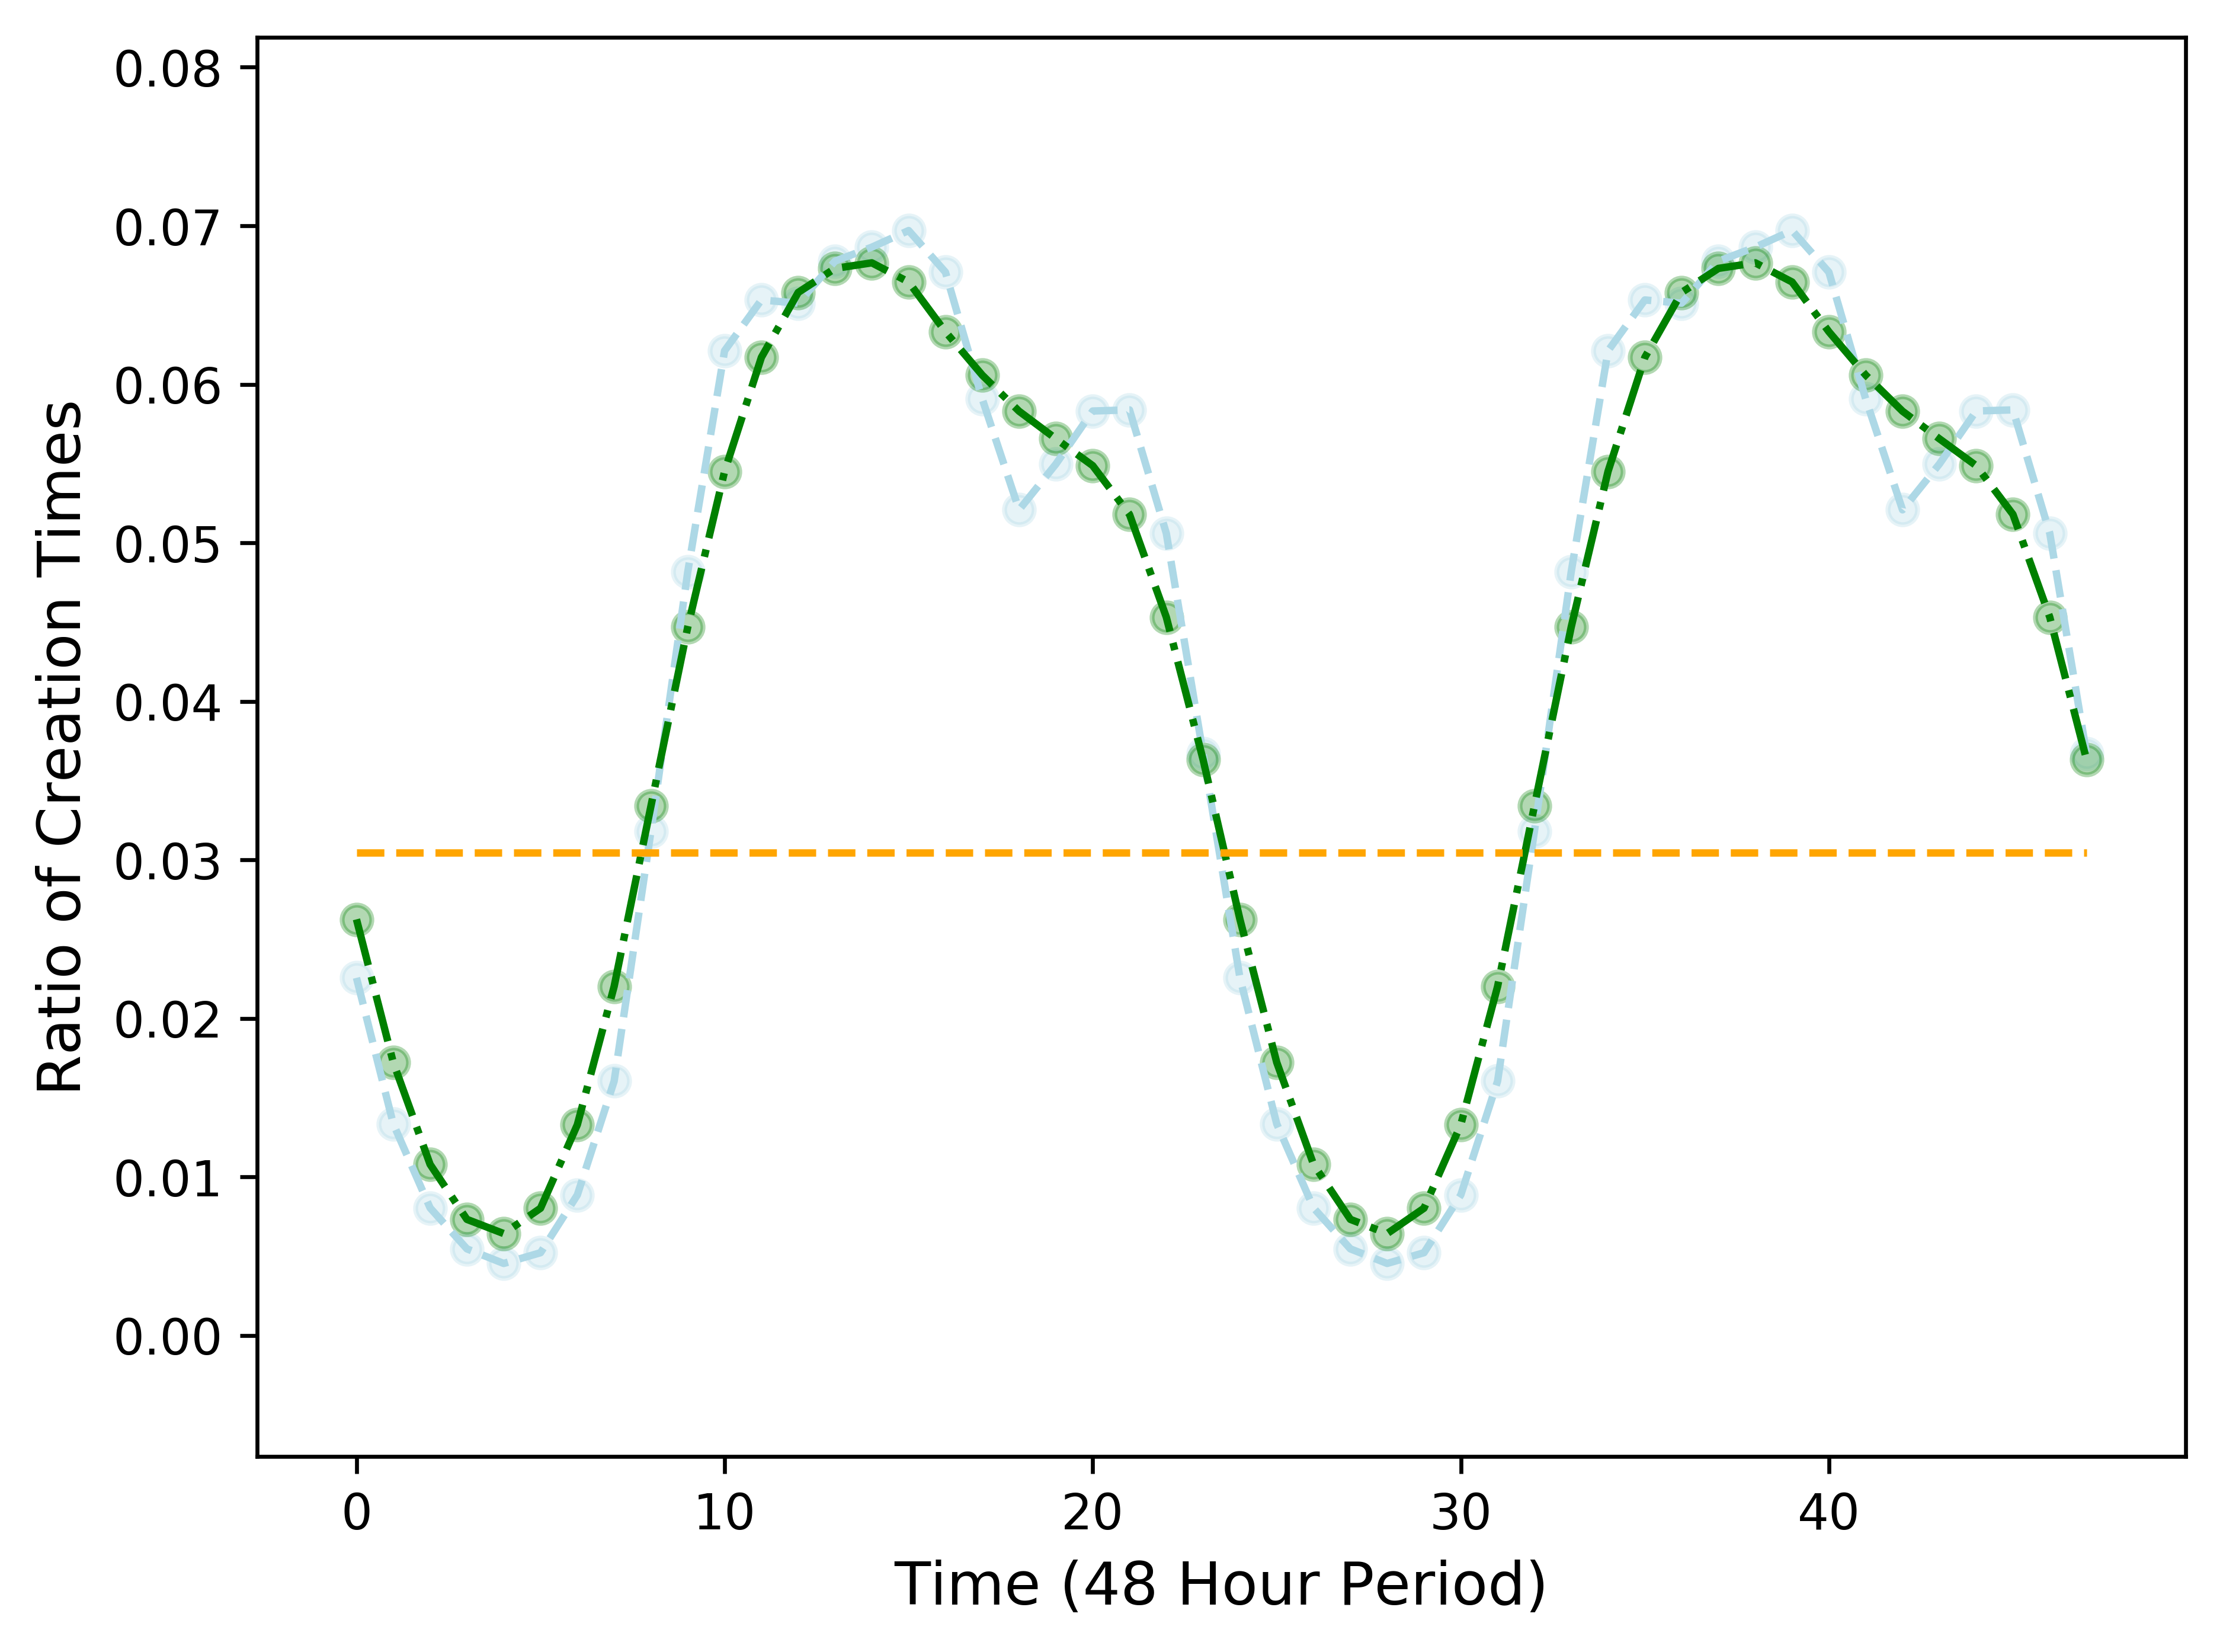
\includegraphics[width=.48\textwidth]{Figures/london.png}}
   \hspace*{\fill}   % maximize separation between the subfigures
   \subfloat[self-reported location `losangelesca']{\label{fig_1b}
      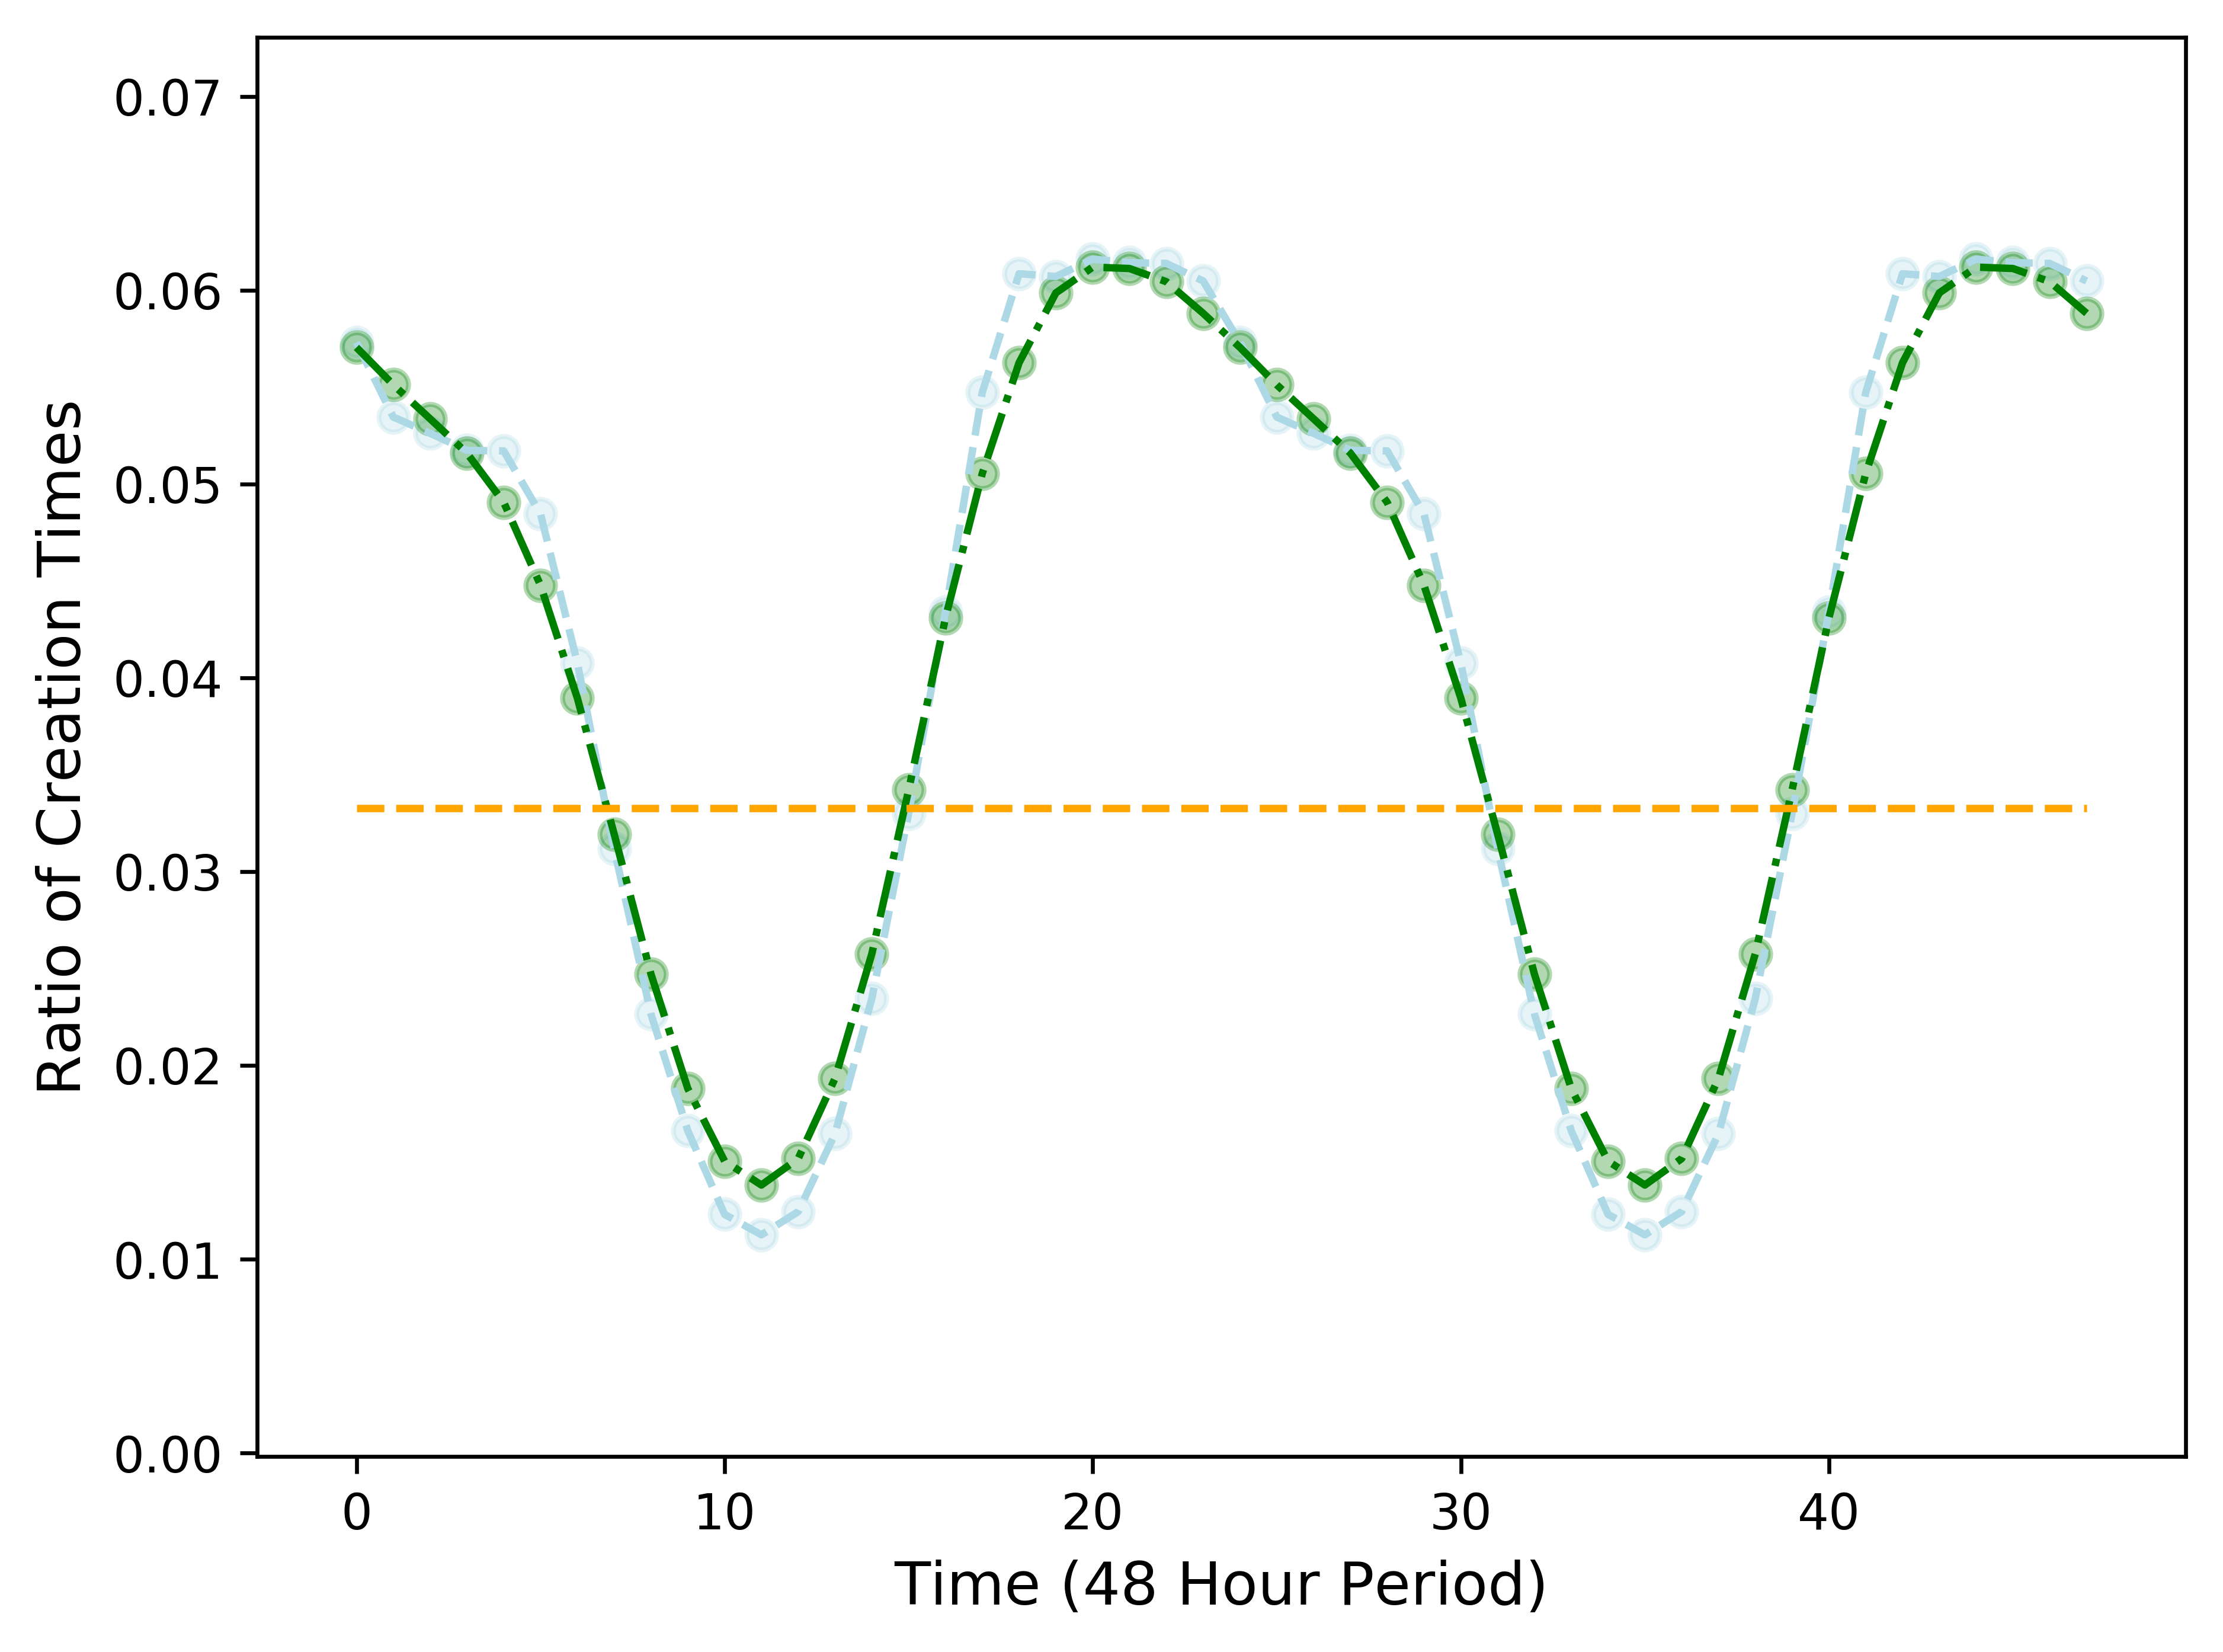
\includegraphics[width=.48\textwidth]{Figures/losangelesca.png}}
   \caption[Example Time Distributions]{Normalized 48-hour histograms using creation times of users from (a) `london' and (b) `losangelesca' are shown. The blue curve shows the original time distribution, and the green curve represents the moving average (with $n=5$). The orange line corresponds to the threshold below which the potential sleep cycle is identified from the green curve. The mins between the two charts are 7-9 hours apart matching expectation in that the time difference between the two locations is 8 hours.} \label{fig_1}
\end{figure*}

As an illustration, Fig. \ref{fig_1} shows the $f(t)$ formed from creation times corresponding to users associated with %that use 
locations (a) `london' and (b) `losangelesca'. %The $f(t)$ may be uneven, see blue lines in Fig. \ref{fig_1}, 
The data (%shown with 
blue lines) is noisy, and to achieve smoothness we compute moving averages (with $n=5$ consecutive points), % moving average which are 
depicted by green lines.% in the figure. % and clearly they are much smoother. 
The orange line corresponds to the threshold below which the potential sleep cycle is identified from the green curve.

%User group or message traffic that is originating from a specific time zone will result in a time distribution that has a U-shaped parabola. The U-shaped parabola 
It is assumed that the regions around the minima (in the smoothed curve) correspond to 
a nocturnal period when many residents of the region sleep, and hence are not active on social media.
%corresponds to the night time in the specific time zone and for this reason there is less activity. 
This region, expected to be an 8-hour period (a third of the 24-hour cycle) % is expected to be devoted to sleep. The sleep portion of the 24-hour cycle can be 
is identified using the threshold %of  $f(t)$ %is below the percentile
$p=33\%$ in Fig. \ref{fig_1}). 
%The sleep cycle %for bottom chart
%occurs between %the first and second intersection points of this threshold.
%and for top it is between the second and third intersection points. 
The portion of the smoothed curve below the threshold can be approximated by a quadratic function. Minimum of the quadratic used to predict the UTC offset; confidence in which increases with the coefficient of determination $R^2$ and the magnitude of the power coefficient $c_2$ ($c_2$ close to zero associated with a flat like sleep cycle with not as clear a minimum).
% function %and if it is a U-shaped parabola to make a UTC prediction. 
We record (i) the predicted UTC offset, (ii) the power coefficient $c_2$,  and (iii) the coefficient of determination $R^2$.

The next subsection addresses the selection of  parameters for the moving average $n$ and the percentile $p$ threshold,
and describes the linear regression leading to the computation of UTC.
%work the best and how the e
%Equation (\ref{eq001}).

\subsection{Parameter Determination} \label{parameterDeter} 

Instead of using the entire $|G|$ creation times of the group, we use a method akin to bootstrapping %(see Efron and Tibshirani~
[\ref{appendix:bookCh28}]). Random samples of size $M$ are drawn from $G$, $N$ times, and for each sample, the PST is calculated. 
Over $N$ trials, the average PST is denoted $\mu_G({PST})$, 
and $\sigma_G({PST})$ denotes the standard deviation. %of PSTs over $N$ samples is calculated; denoted by  and
 %, respectively. 

These estimates depend on the 
 choices of the sample size $M$, the number of samples $N$, the size of moving average window $n$, and the sleep cycle threshold percentile $p$. %below which relative frequency $f(t)$ is considered to belong to sleep cycle %are crucial in determining appropriate 
%can affect the estimated value of $\mu_G({PST})$. 
%In order to find the most appropriate values of these parameters, w
We performed multiple experiments, with values of $M=[100, 250, 500, 1000]$, $N=100$, $n = [1, 2, ..., 7, 8]$ and $p = [20, 25, 30, 33, 35, 40, 45]$. %A straight line fit
Linear regression was performed for PST vs. $UTC^L$ using least squares estimation, %in the same way 
as shown in Fig. \ref{fig_3}. To measure the performance of selected values of the parameters \emph{Recall, Precision,} and \emph{F1} measures were calculated: 

$${Recall} = \frac{\mbox{\# of user groups where PST-estimate calculated}}{ \mbox{the number of user groups}},$$

$${Precision} = \frac{\mbox{\# of correct UTC predictions}}{\mbox {\# of UTC predictions}},$$

$$F1=\frac{2 \times {Precision}\times {Recall}} {{Precision + Recall}}.$$ 
%Initially, predictions that were more than $t_1=0.5$ away from $UTC^L$ were marked as incorrect. The $\mu_G({PST})$ and $\sigma_G({PST})$, for all correct predictions were evaluated as 0.3318 and 0.0794, respectively. This provides a threshold $t_2= 0.3318 + 2 \times 0.0794 = 0.4906$ beyond which the group standard deviation is considered too large. Such a group is considered too noisy to generate an accurate PST and, therefore, associated prediction is not considered valid. Out of 12,271 locations 1149 (9.36\%) were identified as noisy. When we evaluated the PSTs for these noisy groups 65.36\% produced a PST that is indeed more than $t_1=0.5$ away from its $UTC^L$.
%Note: in conference paper we discussed how threshold t_3 was formed (this threshold was applied because we did not have a global vs. local classifier in place). t_3 is not needed for current publication and just adds confusion

\begin{figure*}[htp]
   \subfloat[F1 for $n$ and $p$]{\label{fig_2a}
      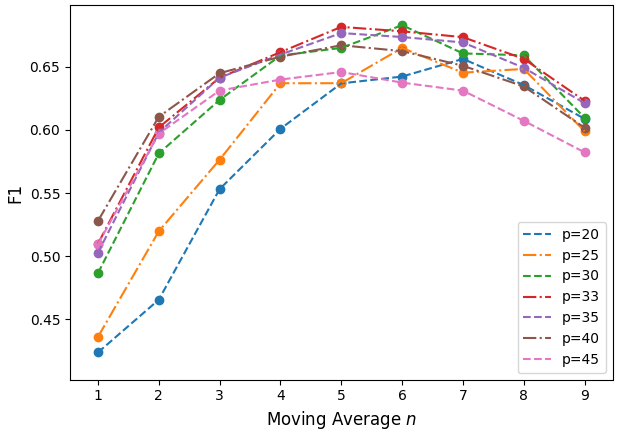
\includegraphics[width=.48\textwidth]{Figures/Fig33.png}}
   \hspace*{\fill}   % maximize separation between the subfigures
   \subfloat[Precision for $p$ and $M$]{\label{fig_2b}
      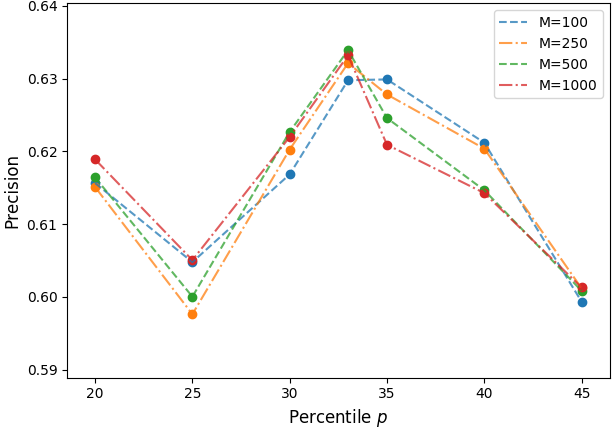
\includegraphics[width=.48\textwidth]{Figures/Fig44.png}}
\\
  \subfloat[Precision for $n$ and $M$]{\label{fig_2c}
      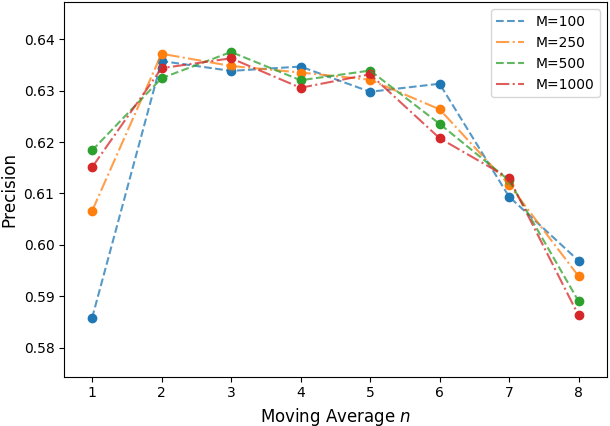
\includegraphics[width=.48\textwidth]{Figures/Fig55.png}}
  \hspace*{\fill}   % maximize separation between the subfigures
  \subfloat[Precision for group size $x$ and $M$]{\label{fig_2d}
      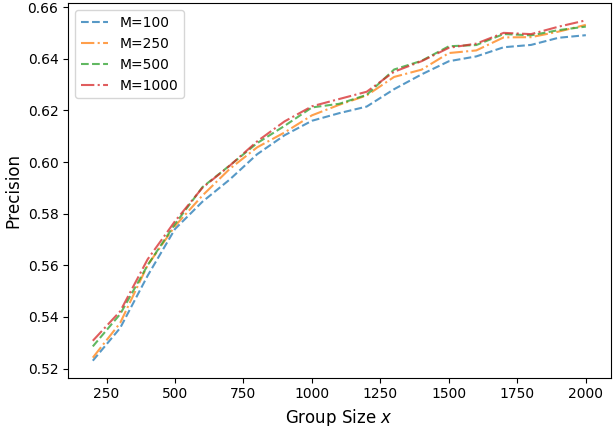
\includegraphics[width=.48\textwidth]{Figures/Replacement.png}}
   \caption[Identifying Best Parameters for Time Distribution]{Variation of ability to predict $UTC^L$ ($t_1=0.5$) with parameter values: (a) F1 vs. moving average window width $n$, for different values of percentile $p$, fixing $M=250$; (b) Precision vs. percentile $p$, for  different sample sizes $M$, fixing $n=5$ which yielded the best F1 score; (c) Precision vs. $n$ for different values of $M$, fixing $p=33$ which yielded the best F1 score; and (d) Precision vs. group size $x$
for different values of $M$, using sampling with replacement, and fixing  $p=33$ and $n=5$.} \label{fig_2}
\end{figure*}

Predictions that were more than $t_1=0.5$ away from $UTC^L$ were marked as incorrect. The following observations emerge from Fig. \ref{fig_2}:

\begin{itemize}
    \item 
Fig. \ref{fig_2}(a) shows F1 for different values of $p$ and $n$ for $M = 250$ and $t_1=0.5$ over all groups in the UTC offset dataset. It can be seen that the best performance with F1 = 68.14\% is achieved using $p=33$ and $n=5$.  
\item
Fig. \ref{fig_2}(b) confirms that $p=33$ is the best performing using precision for four different values of $M$. This value of $p$ is also an intuitive choice because, as mentioned earlier, about a third of the 24-hour period is expected to be devoted to sleep. Smaller percentile ($p<30$) reduces the associated sleeping cycle and it is harder to fit a parabola and to get a good UTC offset prediction. On the other hand, if $p$ is too high ($p\geq40$) then points that are outside of the sleeping cycle will be incorporated causing the performance to suffer. 
\item
%The effect of $n$ is to smooth out the curve, 
Fig. \ref{fig_2}(c) shows that $n \in [2,5]$  exhibit high precision for all values of $M$. From this figure, we conclude that any choice of $n\in [2,5]$ is reasonable to smooth out irregularities, preserve high precision, but is not too high to delete the sleep cycle from the time distribution. However, considering both, the precision and F1,  we conclude that $n=5$ is the best choice. 
\item
When using sample size $M$ the group size needed to be at least $M$ because we have used sampling without replacement. Sampling with replacement allows to better understand whether improvement comes from a bigger sample size or a bigger group size. 
Fig. \ref{fig_2}(d) shows performance for sampling with replacement across different $M$ values as the group size increases (using $n=5$ and $p=33$). We conclude that 
performance is not affected by $M$,  although performance improves with group size.
\end{itemize}

\begin{figure}[!t]
\centering
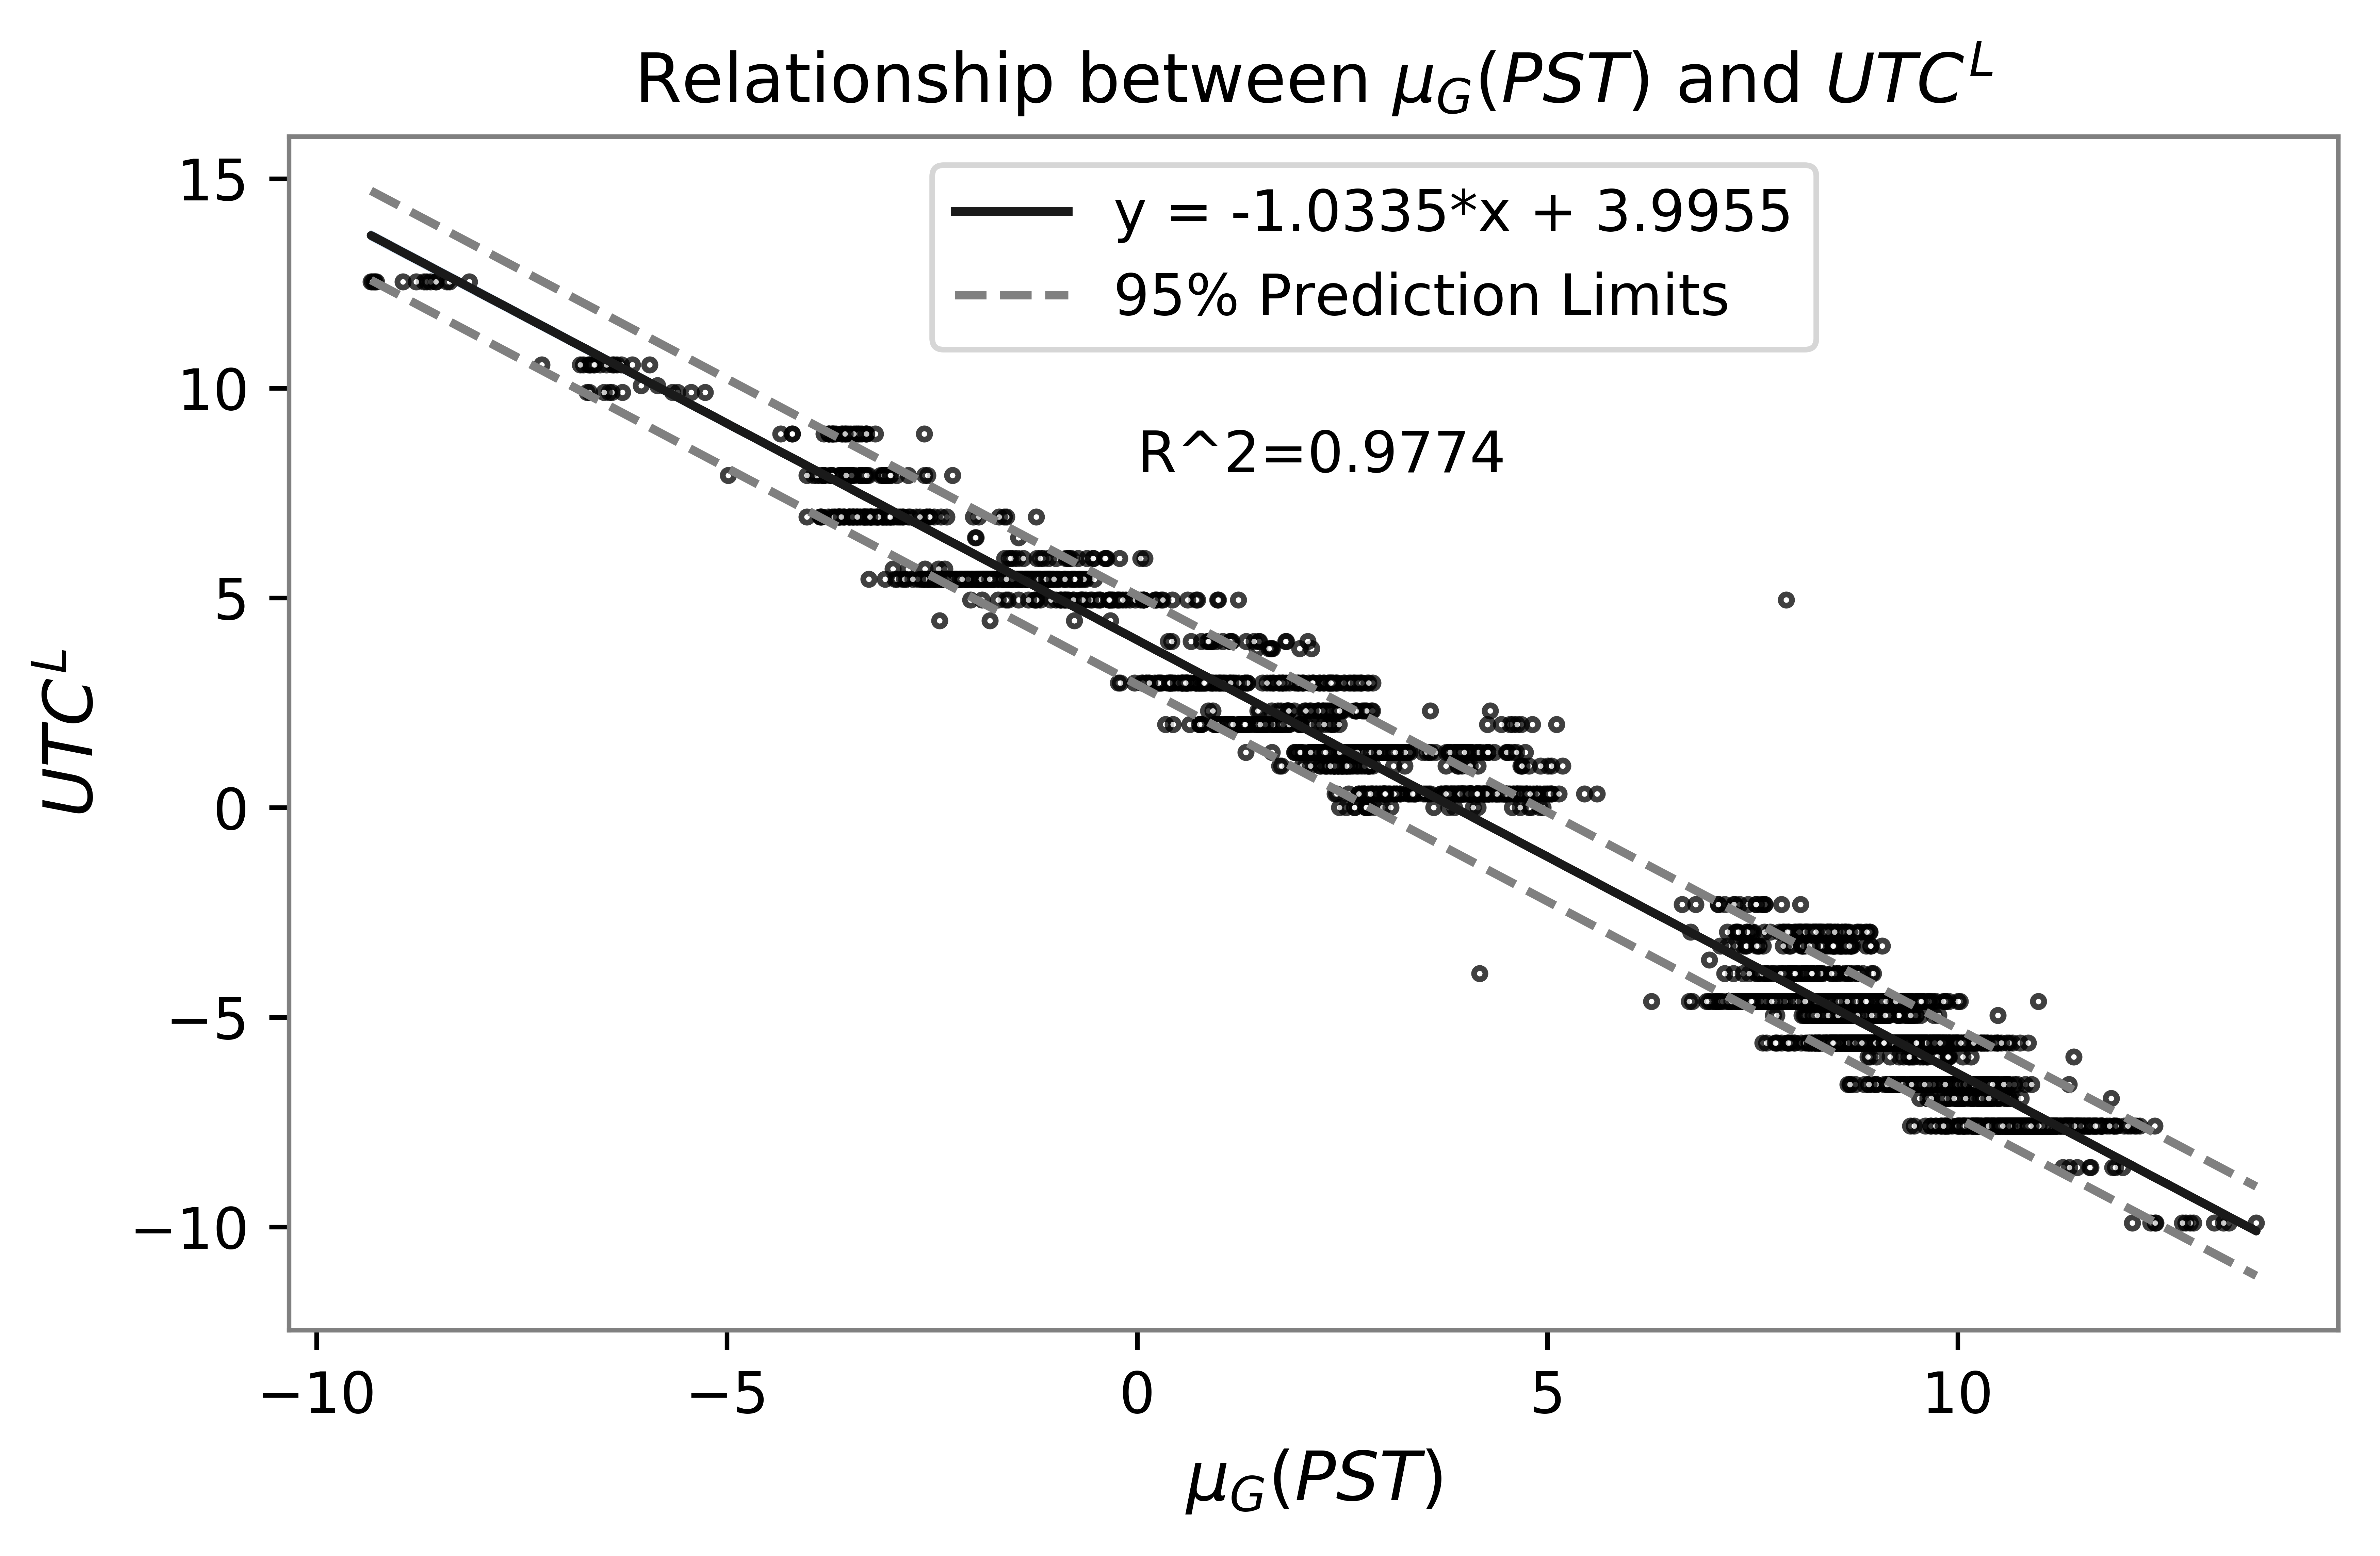
\includegraphics[width=5in]{Figures/filename.png}
\caption[Linear regression between UTC and min of time distribution]{Result of linear regression performed on data points with known geolocation, plotting $UTC^L$ against
$\mu_G({PST})$, with $M=250$, $n=5$, $p=33$, and group size exceeding 1000.}
\label{fig_3}
\end{figure} 

The plot in Fig. \ref{fig_3} uses $M=250$, $n=5$, $p=33$, and group size equal to at least 1000. Using these parameters the relationship between predicted PST %%%%%% WAS UTC, PLEASE CONFIRM ******* (yes should have said PST)
and actual UTC is shown. A linear relationship can clearly be observed, using $UTC^P = -1.0335\times PST + 3.9955$
 with overall $R^2=0.9774$;
 this is approximated as follows:
% equation (\ref{eq001}):

\begin{equation}
UTC^P = -1.0 \times PST + 4.0
\label{eq001}
\end{equation}

\section{Temporal Analysis of Message Traffic data} \label{sec4}
\label{subsec-illustration}

In this section, we illustrate that time-based features can be used for associating persons and topics with a geographic area. The time-based approach is confirmed using message traffic with coordinates.

%The most data on Twitter can be obtained via the streaming API which gives researchers access to an unfiltered stream of tweets. Once message traffic is collected the user that generates the message and the user mentioned in message is used for inferring the social graph. The graph is used for identifying authorities and closely knit communities. Authorities and communities may be related to a certain geographic area, topic, and/or sentiment towards a topic. Messages with coordinates and place mentions or self-reported locations of the users in the graph can be used to filter to those users that are near a specific geographic area. In this section we illustrate that time-based features can be used for high-level geocoding.

Our focus is on understanding the  spatiotemporal aspects of the
 Twitter social graph, 
 connecting senders of messages and users mentioned in the messages. 
We explore the geographical distribution of senders of 
 messages who mention an individual, 
 thereby evaluating the extent to which an influencer (mentioned in the messages) has global influence.
This is often accomplished by analyzing 
 message traffic data, since the full follower-followee
graph cannot be directly collected due to limitations imposed by the free Twitter API.
%Such a social network can be used to extract many useful properties, such as close knit communities and influencers.
%individuals, etc. 
Messages with coordinates and place mentions or self-reported locations of the users can be used to filter out users that are near a specific geographic area; in this manner, influential individuals and communities belonging to a certain geographic area can be identified.  
%Via streaming API Twitter provides unfiltered access   to an  stream of tweets. From the message traffic data a social graph can be generated using the relation between users that generate the message and users that are mentioned in the message. Such a social network can be used to extract many useful properties, such as identify close knit communities, influential individuals, etc. Messages with coordinates and place mentions or self-reported locations of the users can be used to filter out users that are near a specific geographic area and in this manner influential individuals and communities belonging to a certain geographic area, topic, and/or sentiment towards a topic can be identified.  In this section we illustrate that time-based features can be used for high-level geocoding.

\subsection{Message Traffic Dataset}
We collected five days of message traffic data in the first week of December 2020 for a total of 18.67 million messages. This dataset is denoted as $D_{mess}$. Preprocessing consisted of turning each message to lowercase and tokenizing using NLTK library's TweetTokenizer. For each message, the hour was extracted from its creation time. Each token was associated with a set of hours from the set of messages in which the token appears. Tokens that were at least three characters in length and appeared in over 500 messages were retained, resulting in a total of 23,747 tokens.

\begin{table}[htbp]
\small
\caption{Token labels using messages with geolocation tags}
\label{table_M1}
\centering
\begin{tabular}{|c|c|c|c|c|c|}
\hline
\bfseries Token & \bfseries Label & \bfseries NA\_SA & \bfseries AF\_EUR & \bfseries AS\_OC & \bfseries Total\\
\hline
@realdonaldtrump & NA\_SA & 537 & 47 & 19 & 603\\
\hline
@joebiden & NA\_SA & 142 & 14 & 6 & 162\\
\hline
\#oath4ssr & AS\_OC & 18 & 2 & 30 & 50\\
\hline
@narendramodi & AS\_OC & 1 & 0 & 47 & 48\\
\hline
\#gfvip & AF\_EUR & 0 & 35 & 0 & 35\\
\hline
@pmoindia & AS\_OC & 0 & 1 & 33 & 34\\
\hline
@thehill & NA\_SA & 25 & 2 & 0 & 27\\
\hline
@jairbolsonaro & NA\_SA & 27 & 0 & 0 & 27\\
\hline
@nytimes & NA\_SA & 21 & 3 & 3 & 27\\
\hline
@llinwood & NA\_SA & 24 & 1 & 1 & 26\\
\hline
\end{tabular}
\end{table}

\iffalse
\begin{table}[htbp]
\small
\caption{Token labels using messages with geolocation tags}
\label{table_M1}
\centering
\begin{tabular}{|c|c|c|c|c|c|c|}
\hline
\bfseries Token & \bfseries Label & \bfseries NA\_SA & \bfseries AF\_EUR & \bfseries AS\_OC & \bfseries Total & \bfseries Label Ratio\\
\hline
@realdonaldtrump & NA\_SA & 537 & 47 & 19 & 603 & 0.89\\
\hline
@joebiden & NA\_SA & 142 & 14 & 6 & 162 & 0.88\\
\hline
\#oath4ssr & AS\_OC & 18 & 2 & 30 & 50 & 0.6\\
\hline
@narendramodi & AS\_OC & 1 & 0 & 47 & 48 & 0.98\\
\hline
\#gfvip & AF\_EUR & 0 & 35 & 0 & 35 & 1\\
\hline
@pmoindia & AS\_OC & 0 & 1 & 33 & 34 & 0.97\\
\hline
@thehill & NA\_SA & 25 & 2 & 0 & 27 & 0.93\\
\hline
@jairbolsonaro & NA\_SA & 27 & 0 & 0 & 27 & 1\\
\hline
@nytimes & NA\_SA & 21 & 3 & 3 & 27 & 0.78\\
\hline
@llinwood & NA\_SA & 24 & 1 & 1 & 26 & 0.92\\
\hline
\end{tabular}
\end{table}
\fi

Messages that contain location coordinates %then we know where it originated from. 
%This allows us to build the
provide ground truth against which we can evaluate UTC-based predictions. 
Such messages comprised only 0.71\% of all messages in our dataset, consistent with other literature suggesting that the number is less than 1\% [\ref{appendix:1.8}]. 
In our dataset, there were 6,632 messages with point coordinates and 126,765 messages with a place coordinate (bounding box).  


Among 23747 tokens, as many as 20252 were contained in at least one message with coordinates. 
For each token, we record the number of messages that came from the Americas (longitude $\leq$ -25), Europe/Africa (-25 $<$ longitude $\leq$ 65), and Asia/Oceania (longitude $>$ 65). 
For coordinates specified using a bounding box, both the longitude components had to be associated with the same region. A token was assigned a label based on the region which captured the biggest ratio of messages. 
Among the 20252 tokens with coordinate information, we found that 11955 were associated with the Americas, 4991 with
 Europe/Africa, and 3306 with Asia/Oceania. 
 Table \ref{table_M1} shows examples of ground truth generated in this fashion that contain topic or person mentions (NA\_SA = Americas, AF\_EUR = Europe/Africa, and AS\_OC = Asia/Oceania). The number of messages with coordinates are shown for each region and token. The region that captures the most messages is chosen as the label. For example, for @realdonaldtrump the NA\_SA is the label since 537 messages are from it vs. only 47 and 19 for the other regions.

%For each such token its corresponding frequency was calculated. 
%\subsection{Predict Top Trending Tokens by Region using UTC}\label{ms-prediction}
%We went through all the messages where a specific token appears in order to record the hours and use those to generate a time distribution. Those tokens for which a U-shaped parabola could be fitted were recorded along with the associated (i) the predicted UTC offset, (ii) the coefficient $c_2$ and (iii) the coefficient of determination $R^2$.
%The bigger the $R^2$ the more confidence we have in the fitted polynomial. However, a small $c_2$ represents lack of U-shape. 
%\subsection{Identifying Tokens Region}  \label{ms-prediction} Temporal distribution of a specific token can be obtained using the times of associated messages. As in the previous section, we applied the algorithm to identify whether or not U-shaped parabola could be fitted to this distribution and obtained the associated (i) the predicted UTC offset, (ii) the coefficient of the quadratic term, $c_2$ and (iii) the coefficient of determination $R^2$. As before large value of $R^2$ implies more confidence in the fitted polynomial and small $c_2$ represents lack of U-shapeliness. 
\subsection{Predicting Region of Token}  \label{ms-prediction}

We extracted the  hours (from the creation time) associated with all messages in which each token appears. The set of hours  was used to obtain a time distribution and corresponding: (i) predicted UTC offset, (ii) coefficient of the quadratic term, $c_2$, and (iii) coefficient of determination $R^2$ (using the approach in Section 3.2). As before, a large value of $R^2$ implies  greater confidence in the fitted polynomial, and a large $c_2$ indicates  greater localization of influence.

\begin{figure*}[htp]
   \subfloat[Americas]{\label{fig_M1a}
      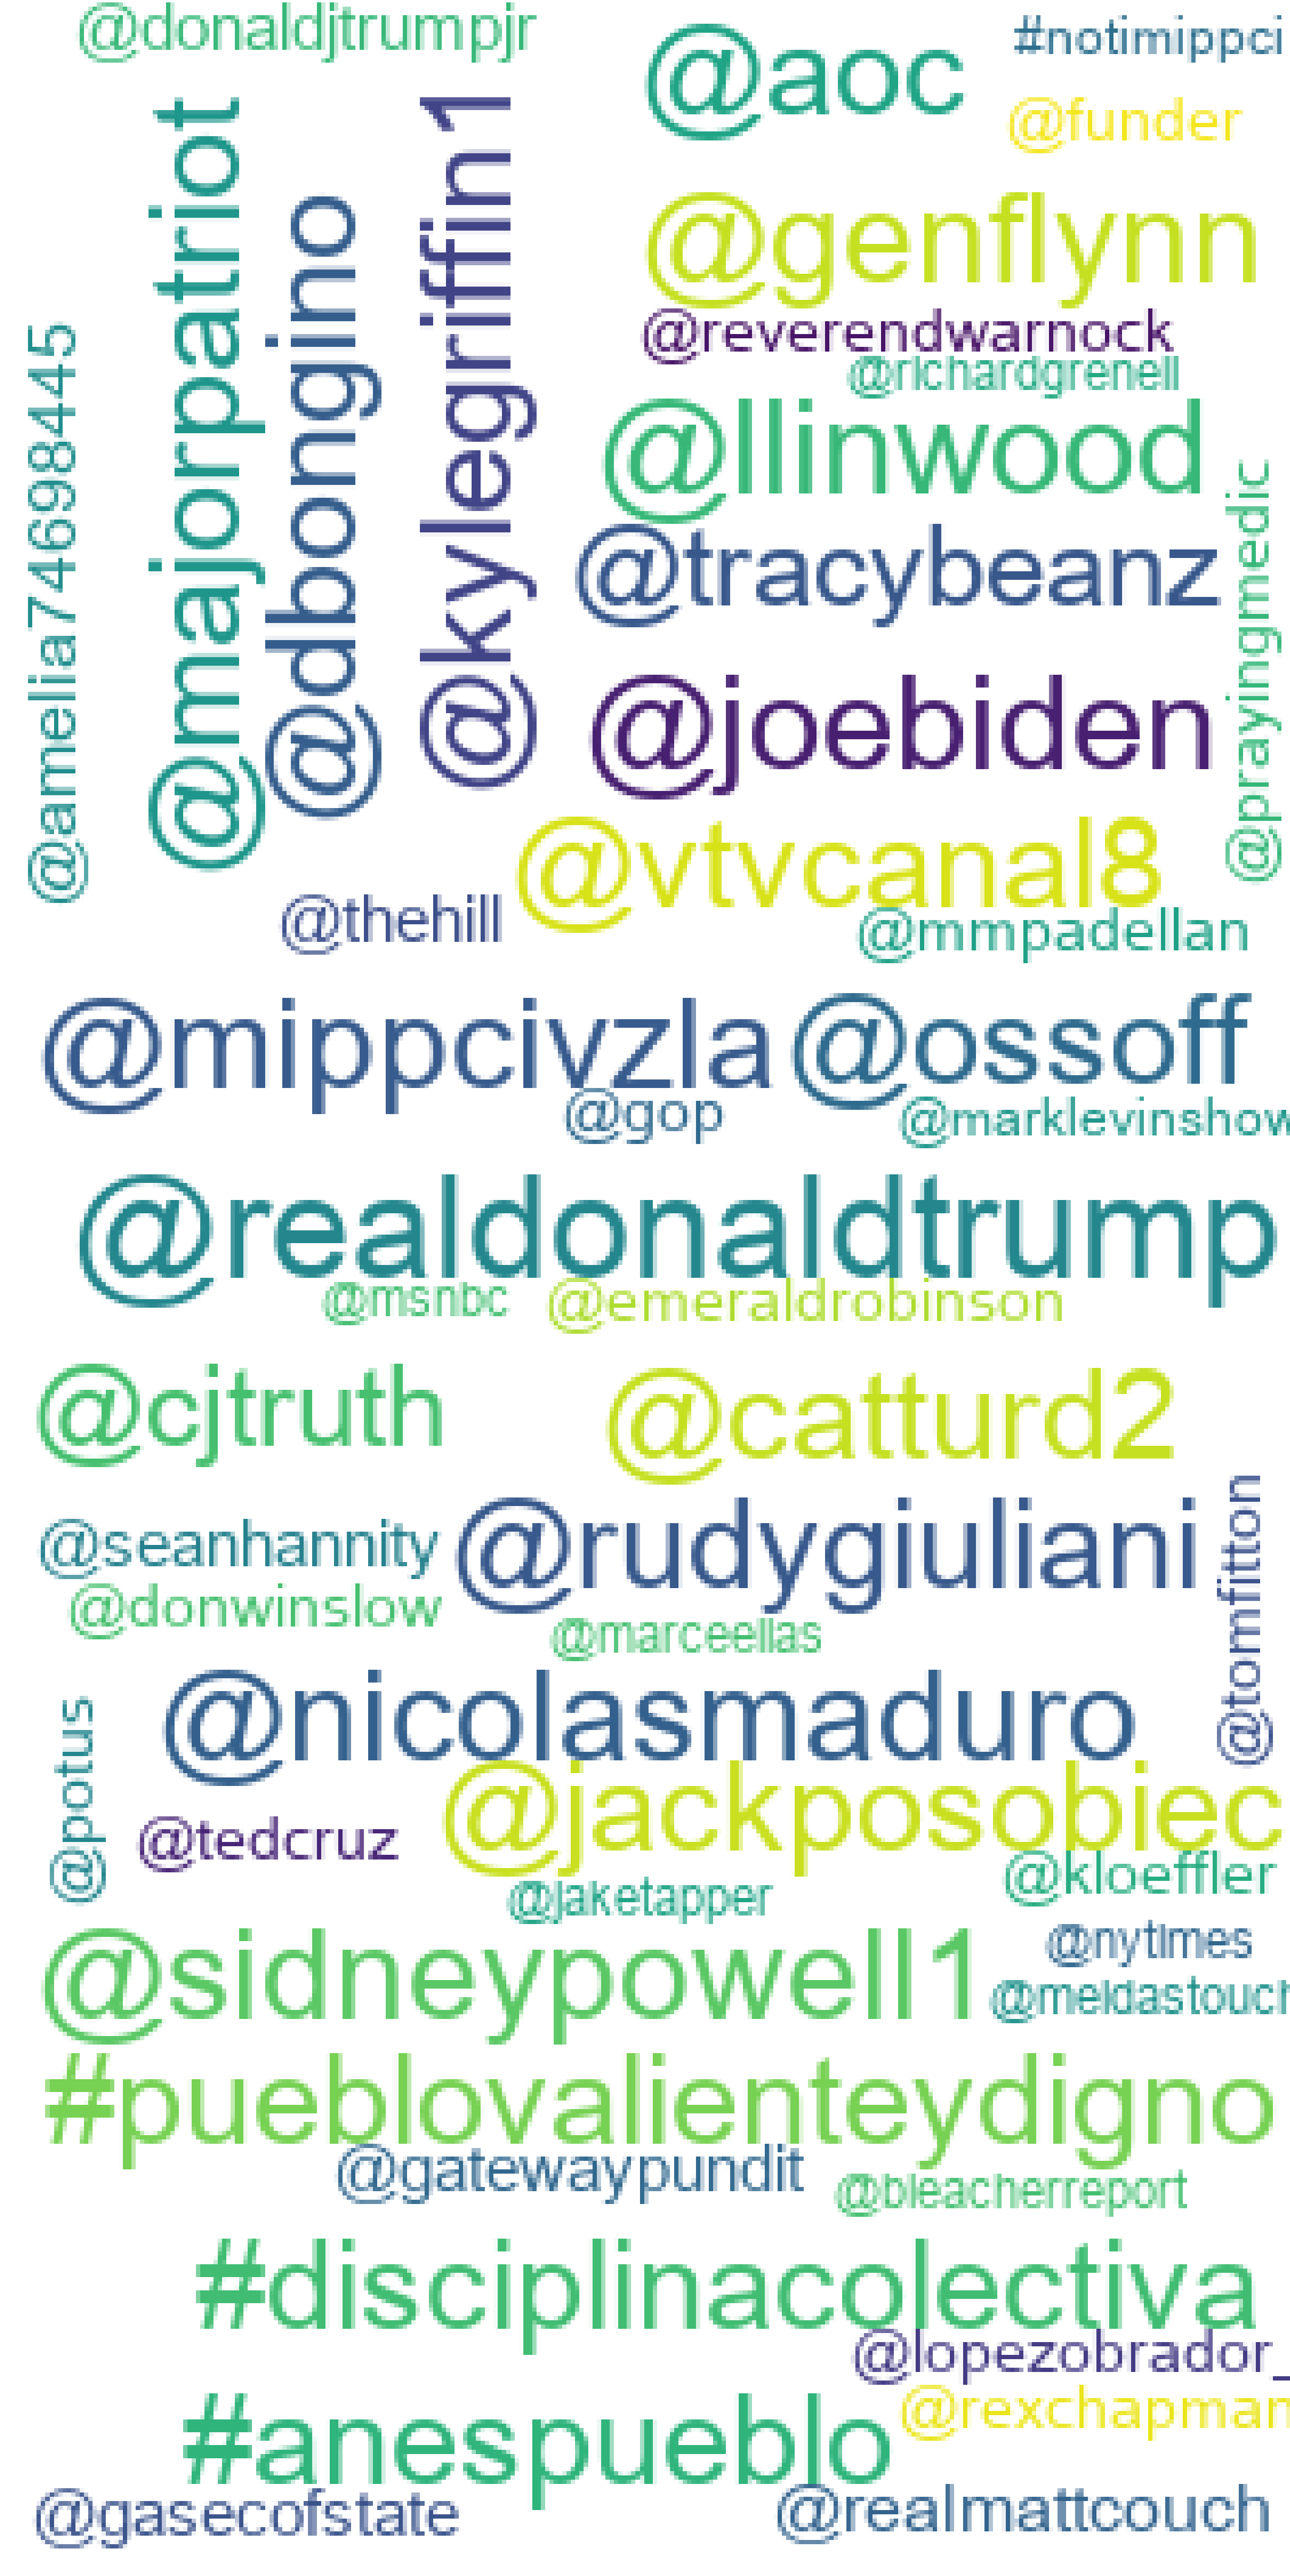
\includegraphics[width=.27\textwidth]{Figures/w1Americas.png}}
   \hspace*{\fill}   % maximize separation between the subfigures
   \subfloat[Europe/Africa]{\label{fig_M1b}
      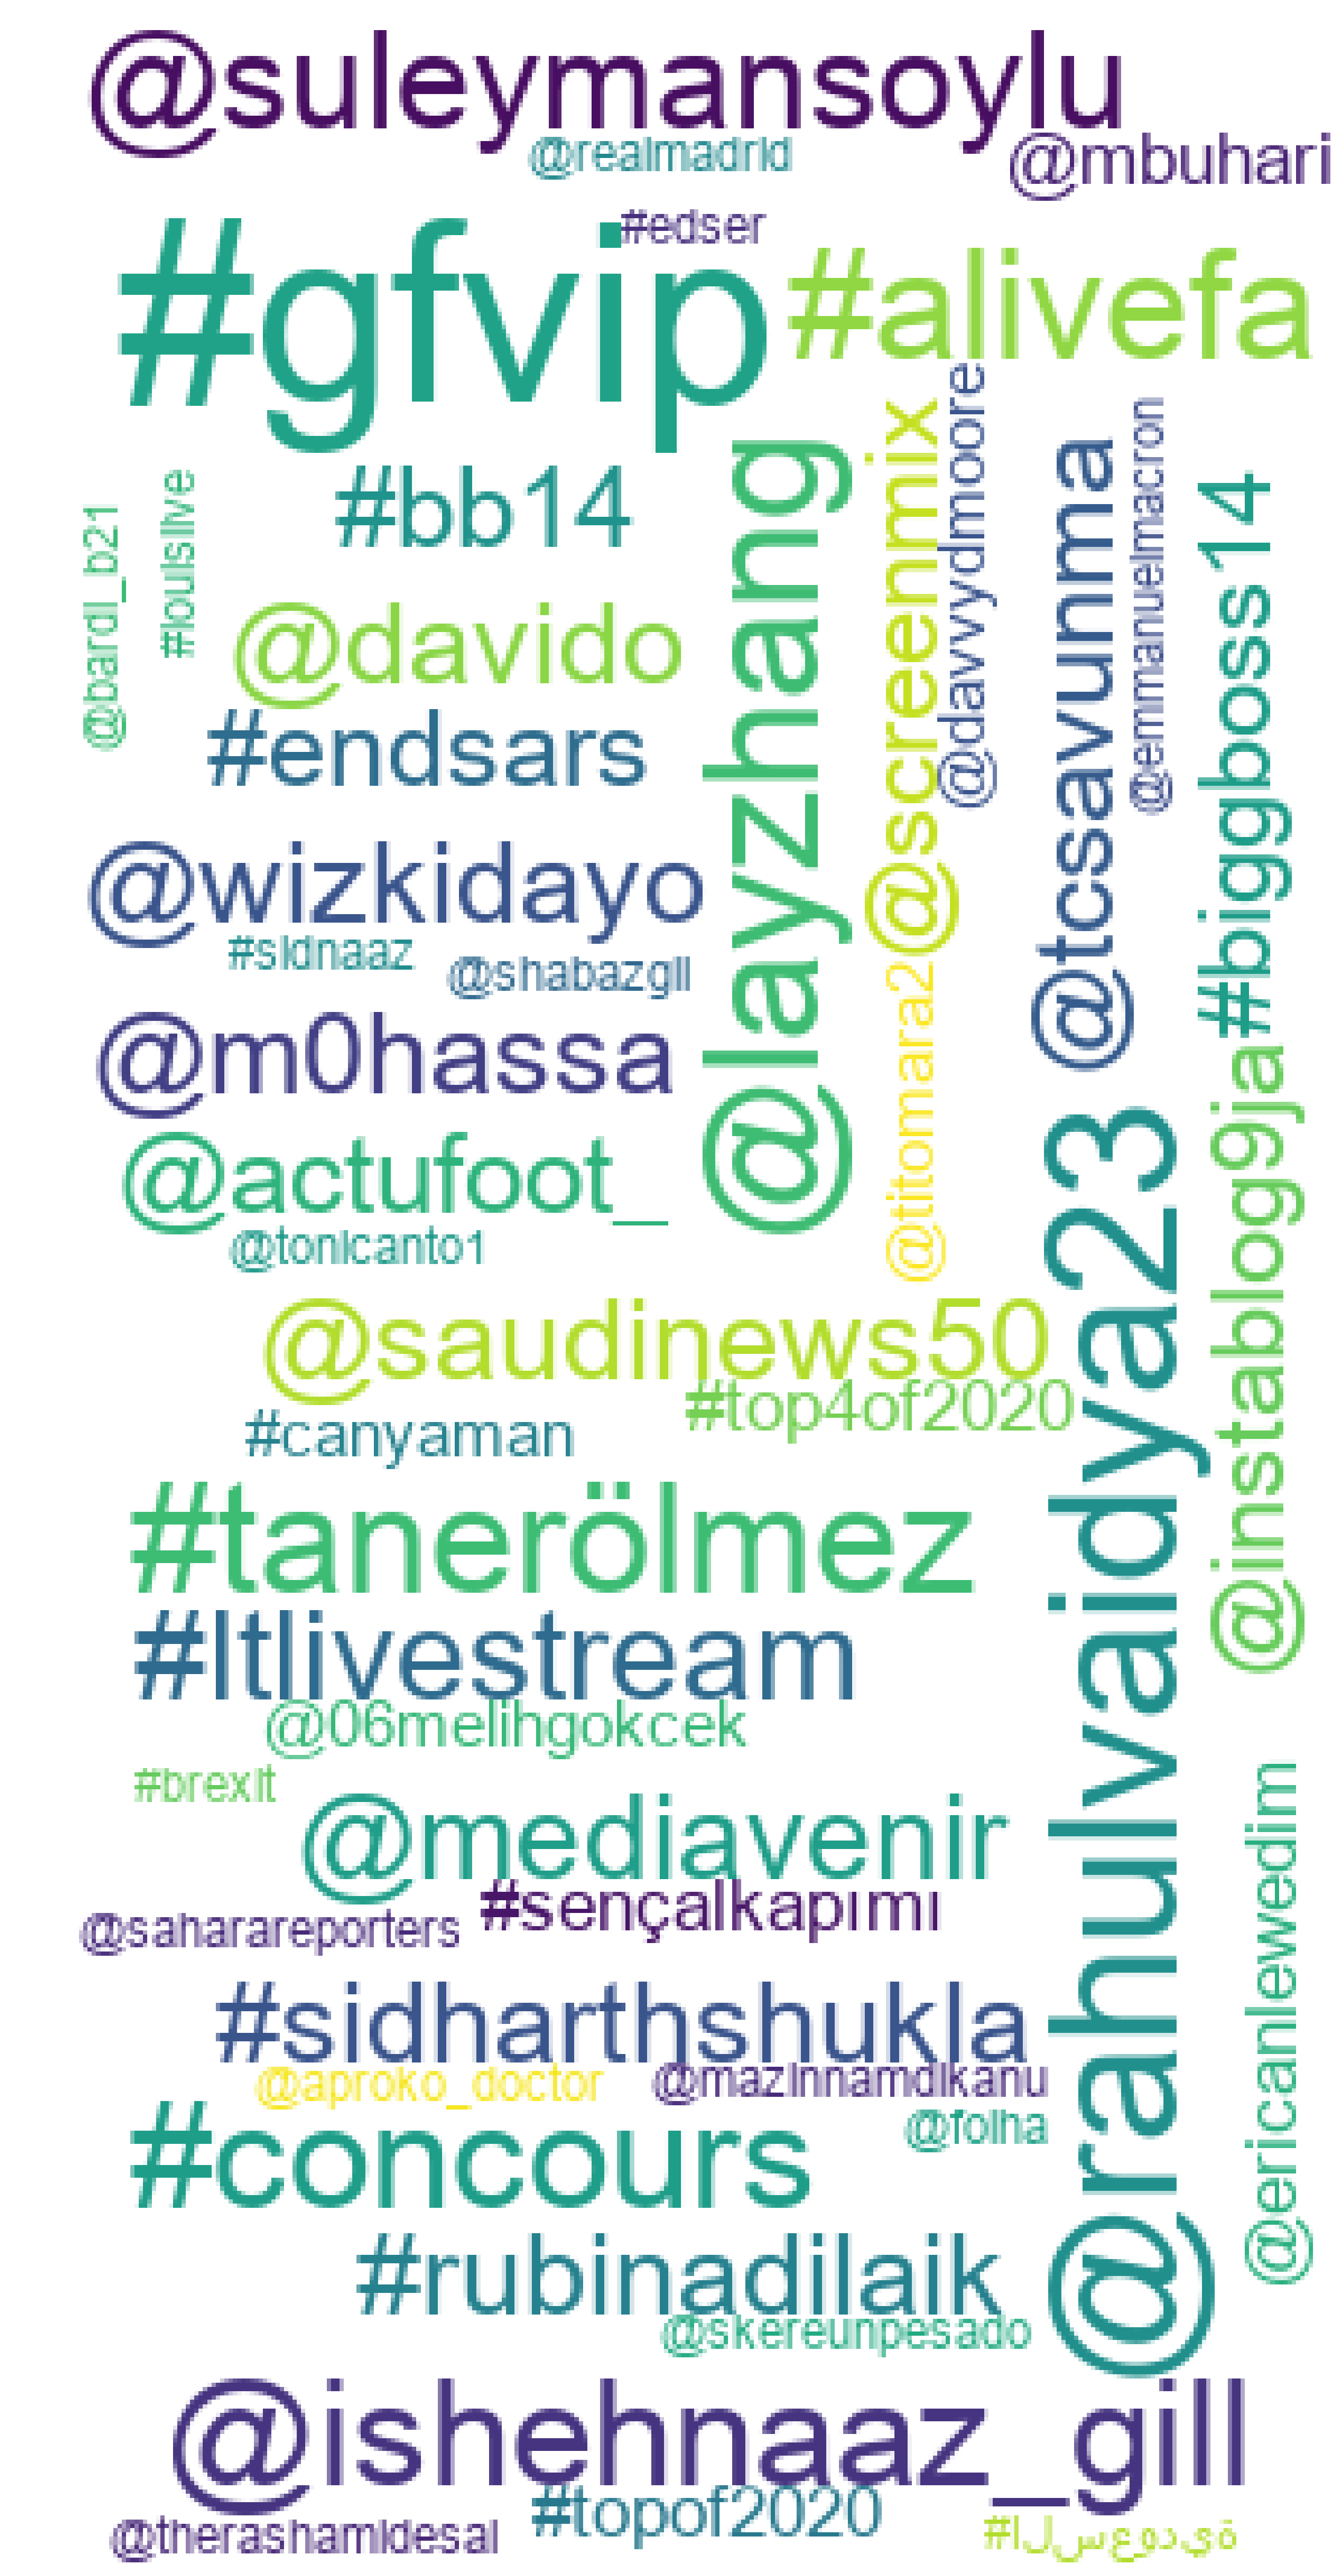
\includegraphics[width=.29\textwidth]{Figures/w3Europe_Africa.png}}
  \hspace*{\fill}   % maximize separation between the subfigures
  \subfloat[Asia/Oceania]{\label{fig_M1c}
      
\includegraphics[width=.29\textwidth]{Figures/Asia_Australia.png}}
   \caption[Predicted Region for Top Trending Keywords]{Top trending tokens (topics and persons) for the (a) North and South America, (b) Europe and Africa, and (c) Asia and Oceania. These were identified using UTC prediction from time curve over message creation times containing the token.} \label{fig_M1}
\end{figure*}

%\subsubsection{Stop Words and U-shape determination}
The NLTK library contains a list of stop-words, such as `the' and `has', which are used worldwide. Their temporal distributions are flat and associated $c_2$ is close to zero.  For example, we found that for stop-words the largest $c_2$ was smaller than $0.001$. To further refine our dataset, we considered $c_2 \geq 0.001$. The result was that not only stop-words but other global topics and persons such as \emph{\#covid19} and \emph{@YouTube} were removed. 

Out of 23747 tokens in the dataset, 16744 contained a sleep cycle that could be used to predict a UTC offset. Based on predicted UTC offset the token was assigned one of three regions: (i) North and South America ($UTC\leq -2$), (ii) Europe and Africa ($-2 < UTC \leq 4$), and (iii) Asia and Oceania ($UTC > 4$). The number of tokens associated with each region was (i) 9618, (ii) 3012, and (iii) 4114 respectively. Of the UTC predictions, 15087 had $R^2\geq0.85$ of which 8487 had $c_2\geq 0.001$. Among these 8487 higher confidence predictions 4135, 1416, and 2936 belonged to each region, respectively. 

As an illustration, Fig. \ref{fig_M1} shows the top fifty words in a word cloud for each geographic region,   focusing on higher confidence tokens that start with $\#$ or $@$ %since these have special meaning on Twitter,
(designating topics or persons).

\subsection{Evaluation}\label{ms-evaluation}
For each token, one of the three regions using UTC prediction is compared with the ground truth, and the accuracy of prediction
%The number of times UTC prediction is accurate 
%(correct vs. total predictions)
is recorded as the ratio of correct versus total predictions, for each region. 

Table \ref{table_M2} shows the results for the three regions. 
The first column shows the type of restrictions placed on a token, % which is 
based on (i) $R^2$ of the polynomial over corresponding sleep cycle, (ii) power coefficient $c_2$ from polynomial, (iii) number of minimum messages, $x$, used to build ground truth, and (iv) whether a collection is limited to persons/topics (@/\#). The accuracy of predictions for each region is shown in columns 3-5 (the respective number of predictions per region is shown in the second column).

%Using UTC predictions tokens are classified to one of the three regions, checked against ground truth region, and number of times UTC prediction is accurate is recorded. Ratio of correct versus total predictions provides the accuracy. Table \ref{table_M2} shows results for the three regions. The first column shows the type of restrictions placed on tokens. The prediction accuracy for each region is shown in columns 3-5 (the respective number of predictions per region is shown under second column). The final column provides overall accuracy. No restriction results show that if a sleep cycle is found and a UTC prediction is made it generally has a good accuracy, but that can be further improved as shown in other rows.

\begin{table}[htbp]
\small
\caption{Performance over Message Traffic}
\label{table_M2}
\centering
\begin{tabular}{|l|l|c|c|c|c|}
\hline
\bfseries Restriction & \bfseries Predictions & \bfseries NA\_SA & \bfseries AF\_EUR & \bfseries AS\_OC\\
\hline
None & 9271, 2825, 2602 & 94.56 & 76.14 & 87.78\\
\hline
$R^2\geq0.85$ & 8611, 2426, 2360 & 95.4 & 80.3 & 89.58\\
\hline
$R^2\geq0.85$, $c_2\geq0.001$ & 4008, 1327, 1976 & 98.6 & 89.9 & 95.29\\
\hline
$R^2\geq0.85$, $c_2\geq0.001$, $x\geq5$ & 3304, 810, 967 & 99.21 & 91.98 & 98.24\\
\hline
$R^2\geq0.85$, $c_2\geq0.001$, $x\geq10$ & 2270, 380, 533 & 99.69 & 94.47 & 98.69\\
\hline
$R^2\geq0.85$, $c_2\geq0.001$, @/\# & 261, 61, 137 & 98.08 & 81.97 & 97.08\\
\hline
\end{tabular}
\end{table}

\iffalse
\begin{table}[htbp]
\small
\caption{Performance over Message Traffic}
\label{table_M2}
\centering
\begin{tabular}{|l|l|c|c|c|c|}
\hline
\bfseries Restriction & \bfseries Predictions & \bfseries NA\_SA & \bfseries AF\_EUR & \bfseries AS\_OC & \bfseries Overall\\
\hline
None & 9271, 2825, 2602 & 94.56 & 76.14 & 87.78 & 89.82\\
\hline
$R^2\geq0.85$ & 8611, 2426, 2360 & 95.4 & 80.3 & 89.58 & 91.64\\
\hline
$R^2\geq0.85$, $c_2\geq0.001$ & 4008, 1327, 1976 & 98.6 & 89.9 & 95.29 & 96.13\\
\hline
$R^2\geq0.85$, $c_2\geq0.001$, $x\geq5$ & 3304, 810, 967 & 99.21 & 91.98 & 98.24 & 97.87\\
\hline
$R^2\geq0.85$, $c_2\geq0.001$, $x\geq10$ & 2270, 380, 533 & 99.69 & 94.47 & 98.69 & 98.9\\
\hline
$R^2\geq0.85$, $c_2\geq0.001$, @/\# & 261, 61, 137 & 98.08 & 81.97 & 97.08 & 95.64\\
\hline
%$R^2\geq0.85$, $c2\geq0.001$, $x\geq5$, @/\# & 128, 24, 50 & 100 & 79.17 & 100 & 97.52\\
%\hline
%$R^2\geq0.85$, $c2\geq0.001$, $x\geq10$, @/\# & 51, 8, 22 & 100 & 87.5 & 100 & 98.77\\
%\hline
\end{tabular}
\end{table}
\fi

Table \ref{table_M2} illustrates that the approach using temporal  distribution is successful. 
The first row, with no restriction, illustrates that if a sleep cycle is found and a UTC prediction is made it generally has good accuracy. The accuracy is  high, particularly for those tokens which have ground truth assembled from more messages (larger $x$) and %which are based of
with high confidence UTC predictions (high $R^2$ and $c_2$). 

About 13\% of the tokens that were labeled using UTC did not have any message traffic with coordinates. A bigger collection could be explored, but there is reason to think that some tokens % %concepts  ??????
just won't get a geo-tag assigned. Fewer than 1\% of messages contained geo-tags, and 38\% of the tokens had fewer than $5$ geo-tagged data points; a prediction based on such a small sample is not made with high confidence. On the other hand, time is available for all messages and each token appeared in at least 500 messages giving us greater confidence in the corresponding time distribution.  This illustrates the usefulness of our approach.

Another alternative would be to utilize the self-reported locations of the users that wrote the messages, but %as already discussed
this would require a complex geocoding solution that can handle the different ways persons refer to locations in various %natural 
languages. Using time distributions  is hence %the best
 a better solution for quickly understanding important keywords in message traffic as they pertain to a geographic region of interest.

\subsection{Comparison against Baseline based on Google Trends}

In a recent paper, Zola et. al. [\ref{appendix:bookChNew5}] attempt to estimate worldwide Twitter user locations without relying on geolocation target labels (no geotagged tweets or user location profiles and no access to geographic dictionaries). Their dataset consisted of 744,830 tweets written by 3,298 users from 54 countries. The location of each user was manually verified. Their approach focuses on nouns (like sites, events, people), which are expected to have a spatial context that is helpful for user location estimation. Each noun was associated with a geographic region based on Google Trends (Google Trends identifies nouns that are trending in various cities). For each user, clustering is used to identify the most probable centroid from coordinates associated with each city. Because no geoinformation is used, the problem is more complex; their approach correctly predicts the ground truth locations of 15\%, 23\%, 39\%, 58\%, 70\%, 82\% of the users for tolerance distances of 250, 500, 1000, 2000, 4000, and 10000 km. Our method also does not utilize any geoinformation, relying only on creation times as the feature, and hence it was appropriate to compare our approach against the one based on Google Trends.

In [\ref{appendix:bookChNew5}] the authors utilize the following approach:
\begin{enumerate}
\item Part of Speech Tagging used to identify a set of nouns for each user.
\item Pytrends Python module is used to associate a noun with a list of cities. Google gives each city a weight, from 0 to 100, based on how popular the noun was (based on how many search queries, originating from that city, contained that noun). Cities with scores of zero are given scores of one so that a non-zero value is present for each city. 
\item Google geocoder Python module (used to get lat, long of each city)
\item Scikit-learn Python library (used to get the centroid) the best method is based on K-means and Density-Based Spatial Clustering of Applications with Noise (DBSCAN) 
\item Centroid is compared to the known location of a user. Median, Mean, and ACC@x (is a user within x kilometers of predicted centroid) are recorded across all users.
\end{enumerate}

We attempt to apply Google Trends to our dataset. In our method we also utilize Pytrends. Pytrend is an unofficial library supporting Google Trends. In function interest\_by\_region() in file pytrends/request.py we change the code so that the Pandas data frame is returned immediately after collecting JSON response from Google. We find that Google, at the `City’ resolution, does return coordinates for each city, it is just that Pytrends did not accurately capture this information. In this way, it is not necessary to geocode each city name with steps (2) and (3) combined (this reduces the potential for introducing errors due to additional geocoding).

There are other differences in that we are focused on all tokens (not just nouns) and we already have three predefined regions that the world is broken up into (so the accuracy will be judged based on how well a region is predicted as was done in previous section). Google Trends ranking is used to predict a region for a token using:
\begin{enumerate}
\item  For each token, we record the set of cities A that came from the Americas (longitude $\leq$ -25), set of cities B that came from Europe/Africa (-25 $<$ longitude $\leq$ 65), and set of cities C that came from Asia/Oceania (longitude $>$ 65).
\item  For each set of cities in A, B, C the cumulative score across the cities in each set are recorded. The cumulative score is based on the ranking returned by Google Trends (Google gives each city a weight based on how popular the token was in the city, weight is from 0 to 100).
\item  A token is assigned to a region that captured the biggest cumulative score.
\end{enumerate}

Because our problem involves large geographic regions it is also appropriate to utilize the `Country’ resolution vs. only `City’. Each country is given the average latitude and longitude of its cities.%\footnote{https://github.com/apanasyu/GoogleTrends}. 

When using Google Trends by region, it can be used to focus on trends that were formed over a predefined time in the past. These are the predefined time ranges: past 1 hour, 4 hours, day, 7 days, 90 days, 12 months, 5 years, all (2004-present) (Google Trends does not allow one to enter a custom date range i.e. it has to be one of these values).  Table \ref{table_5new_1} shows that the trends will result in very different country rankings depending on the time range utilized. The set of country codes in the top three results across the three time frames in Table \ref{table_5new_1} are: KE = Kenya, CA = Canada, US = United States, NO = Norway, IE = Ireland, and CN = China. We choose to focus on 1-year time frame since this is the default option.

\begin{table}
\small
\caption[Top Country Ranking for keyword @realdonaldtrump using Google Trends]{Different time ranges result in very different top 10 country ranking, for keyword @realdonaldtrump, using Google Trends.}
\label{table_5new_1}
\begin{center}
\begin{tabular}{|c|c|c|c|c|}
\hline
\bfseries 1 month & \bfseries 3 month & \bfseries 1 year & \bfseries 5 year & \bfseries all\\
\hline
(KE, 100)&(CA, 100)&(US, 100)&(US, 100)&(US, 100)\\
\hline
(CA, 17)&(NO, 100)&(CA, 84)&(CA, 84)&(CA, 72)\\
\hline
(US, 9)&(IE, 93)&(CN, 35)&(CN, 35)&(IE, 31)\\
\hline
(GB, 4)&(US, 59)&(IE, 34)&(IE, 34	)&(SH, 31)\\
\hline
(AF, 0)&(NL, 54)&(NZ, 30)&(NZ, 30)&(NZ, 29)\\
\hline
(AL, 0)&(DE, 22)&(SH, 30)&(SH, 30)&(PR, 23)\\
\hline
(DZ, 0)&(GB, 21)&(AU, 21)&(AU, 21)&(AU, 21)\\
\hline
(AS, 0)&(PL, 17)&(GB, 17)&(GB, 17)&(KE, 19)\\
\hline
(AD, 0)&(IN, 4)&(NO, 16)&(NO, 16)&(CR, 16)\\
\hline
(AO, 0)&(AF, 0)&(KE, 14)&(KE, 14)&(SG, 16)\\
\hline
\end{tabular}
\end{center}
\end{table}

The number of requests to Google Trends is limited. For example, Python Pytrends library states that 60 seconds of sleep between requests is recommended in avoiding the limit (we have verified that the limit is around 1440 requests, which greatly reduces the amount of data that can be collected daily). In our evaluation, we have focused on 3183 tokens that had $R^2\geq0.85$, $c_2\geq0.001$, $x\geq10$ and 459 tokens that are limited to persons/topics (@/\#) (the results for these presented in the previous subsection in second to last and last row, respectively, of Table \ref{table_M2}).

Table \ref{table_5new_2} and Table \ref{table_5new_3} show the results for the three regions at city and country levels for the 459 tokens and 3183 tokens respectively. The first column shows the type of restrictions placed on Google Trends. Restrictions considered were (i) using only the location with the highest ranking, (ii) using the top three locations, (iii) using locations with a weight $\geq$ 50, and (iv) using all locations. The last row shows the results using our approach based on message creation times. The second column shows the number of predictions made for each region. The precision of predictions for each region is shown in columns 3-5. The final column is the total number of predictions. 

\begin{table}[htbp]
\small
\caption{Performance over 459 Twitter Persons and Topics (@/\#)}
\label{table_5new_2}
\centering
\begin{tabular}{|l|l|c|c|c|c|c|}
\hline
\bfseries Restriction & \bfseries Predictions & \bfseries NA\_SA & \bfseries AF\_EUR & \bfseries AS\_OC & \bfseries Total\\
\hline
City using top 1& 1, 3, 5&100&100&100&9\\
\hline
City using top 3& 1, 3, 5&100&100&100&9\\
\hline
City using weight $\geq$ 50& 1, 3, 5&100&100&100&9\\
\hline
City all	& 1, 3, 5&100&100&100&9\\
\hline
Country using top 1&161, 28, 52&95.03&92.86&100&241\\
\hline
Country using top 3&161, 28, 52&95.65&92.86&100&241\\
\hline
Country using weight $\geq$ 50&161, 28, 52&95.03&92.86&100&241\\
\hline
Country all&161, 28, 52&95.03&92.86&100&241\\
\hline
Our Approach using Time & 261, 61, 137 & 98.08 & 81.97 & 97.08&459\\
\hline
\end{tabular}
\end{table}

Table \ref{table_5new_2} shows that, out of 459 tokens, City Google Trends only produced 9 results while Country Google Trends produced 241 rankings. These tokens contained symbols @ and \# which on Twitter have special meaning, but these are not as common when using the Google search engine. As a result, Google does not have enough information for trend analysis for these tokens. 

\begin{table}[htbp]
\small
\caption{Performance over 3183 popular tokens with at least 10 coordinates}
\label{table_5new_3}
\centering
\begin{tabular}{|l|l|c|c|c|c|c|}
\hline
\bfseries Restriction & \bfseries Predictions & \bfseries NA\_SA & \bfseries AF\_EUR & \bfseries AS\_OC & \bfseries Total\\
\hline
City using top 1&2188, 360, 491&78.29&84.72&83.1&3039\\
\hline
City using top 3&2188, 360, 491&80.94&87.5&84.73&3039\\
\hline
City using weight $\geq$ 50&2188, 360, 491&84.32&90.83&84.11&3039\\
\hline
City all &2188, 360, 491&90.81&94.17&89&3039\\
\hline
Country using top 1&2267, 365, 525&64.49&76.16&88.76&3157\\
\hline	
Country using top 3&2267, 365, 525&55.32&75.07&88.38&3157\\
\hline
Country using weight $\geq$ 50&2267, 365, 525&59.51&78.9&87.62&3157\\
\hline	
Country all&2267, 365, 525&56.64&94.79&80.76&3157\\
\hline
Our Approach using Time & 2270, 380, 533 & 99.69 & 94.47 & 98.69 & 3183\\
\hline
\end{tabular}
\end{table}

Table \ref{table_5new_3} is more informative since the 3183 tokens consist of more common keywords and that tend to be associated with a geographic area. Google Trends has information on most of these with 3039 at the city resolution and 3157 at the country resolution. At the city resolution, it is seen that as more cities are considered the precision is gradually going up i.e. performance using just the top city is the worst. On the contrary, the performance using Country Google Trends has better overall performance when using only the top Country. This could be because there are a lot of separate countries in Europe and Africa continent and as a result, this region tends to be heavily favored when using all countries. When looking at precision across all regions our proposed time-based method performs the best with 98.9\% overall precision vs. the best results via Google Trends at 69.88\% at the country resolution and 90.92\% at the city resolution.

\textbf{Other caveats:}

One might need to adjust Google Trends based on population. For example, when resolution is at the country level the keyword `pizza' is given a weight of 100 for the USA and 99 for Canada. If adjusting for population and number of Twitter users present in the USA vs. Canada, it seems that the USA should be weighted more. Also, the regions are based on the popularity of search areas where Google is used, but Google and Twitter do not have the same popularity around the world. Google trends seem to be case insensitive i.e. `day’ and `DAY’ both return the same results.

Country Google Trends always returns a ranking for 250 countries (with most countries given a weight equal to zero). When the resolution is at the city level Google will return only the top $x$ cities. For the 3183 tokens the average was $x=68.78$ +/- one standard deviation of 26.07 (so statistics are not provided for all cities in the world).

City Google Trends associates tokens with city locations with city names and coordinates available. We recorded all unique city names and coordinates, associated by City Google Trends, over 3183 tokens, into set AllCity (5229 cities recorded). Next, each city name from set AllCity was fed to Google Trends and the top city result and its coordinates were recorded. Distance in miles was computed between the coordinates of a city query vs. the top city via Google Trends. As an illustration, Table \ref{table_5new_4} shows example city tokens and the top city association and the distance between the two.

\begin{table}[htbp]
\small
\caption{Example Google Trends top City vs. Known City Query}
\label{table_5new_4}
\centering
\begin{tabular}{|l|l|c|}
\hline
\bfseries Query City (coordinates) & \bfseries Top Trends City (coordinates) & \bfseries Distance\\
\hline
Barcelona (41.385064, 2.173404)& Barcelona (41.3850639, 2.1734035) & 0\\
\hline
Houston (29.760427, -95.369803)&Bellaire (29.7057858, -95.4588299) & 6.5426\\
\hline
Chicago (41.878114, -87.629798)&Norridge (41.9633641, -87.827284) &11.7575\\
\hline
New York (40.712784, -74.005941)&Albany (42.6525793, -73.7562317) &134.4946\\
\hline
Rochester (41.064765, -86.215833)&Rochester (44.0121221, -92.4801989) &378.8369\\
\hline
\end{tabular}
\end{table}

Across 5229 city queries, 440/5229 = 8.4\%  produced no results. Out of 4789 queries with results, the average distance between city query and city via Google Trends was 362.03 miles +/- 1334.97. ACC@100 was at 87.57\% illustrating that the majority of cities get matched up to a city within 100 miles. However, it is important to highlight that Google Trends is not the same as geocoding i.e. Chicago using geocoder would not get matched up to Norridge, it is just that there were many queries containing Chicago from that location. Similarly, a query such as `Moscow' will not get associated with Moscow Russia because users there will most likely utilize the Cyrillic alphabet. Cities that are popular travel destinations will also be affected.

In summary, Google Trends is an interesting dataset that could be complementary to the time features proposed. The time features were illustrated to perform better for the proposed task, but Google Trends does have interesting properties. The limitations of Google Trends are related to (i) unavailability of data for certain tokens such as popular Twitter topics/persons, (ii) Google Trends is restricted to about 1400 queries per 24-hour period, and (iii) it is not possible to customize the date range over which trends are formed.

\section{Evolving Popularity: Inferring Daily Changes in Number of Followers} \label{sec5}

It is important to understand how an individual's influence changes with time; this can help predict future influence as well. To predict the future one must first understand the past. In the context of Twitter, the corresponding problem involves estimating the rate at which an influencer has gained their existing followers over a given time period. In this section, we propose a novel algorithm to address this problem, using the creation times of an influencer's followers.

To find the number of followers an influencer has gained on a daily basis (i.e., within a span of 24 hours) during a period of $d$ days, one would need $d+1$ daily collections.
Since this is a time-expensive proposition and because Twitter API doesn't allow one to go back in time,   we propose an alternative method for approximating daily gains for  an influencer, and compare it with an approach based on Meeder, et al. [\ref{appendix:5.15}].

\subsection{Dataset: Stable, Global, Growing Influencers}

Each Twitter user's profile contains the number of followers that the user currently has. By collecting user's profile multiple times we can get a sense for how the number of followers is changing. Let $\psi(i, t)$ represent the number of followers of influencer $i$ at time $t$. Let $\psi(i, t_0, t_1)=\psi(i, t_1)-\psi(i, t_0)$ represents the number of new followers $i$ gains during the  time  interval $[t_0, t_1]$; the number of followers stated in influencer's profile at $t_1$ minus the number of followers stated in influencer's profile at $t_0$. 

Twitter keeps track of popular influencers via \emph{@verified}. There are over 300K verified influencers as of this writing. Our focus is on global stable verified influencers that continue to gain followers; to this end, we collected data on influencers that met the following criteria. The influencer:
\begin{enumerate}
    \item having greater than a million existing followers, i.e., $\psi(i,t)>10^6$;
    \item gaining at least a thousand followers within 24 hours,i.e., $\psi(i, t_0, t_1)\geq10^3$ where $t_0$ and $t_1$ are 24 hours apart; 
    \item the gain in the number of followers is less than 1\% of the overall existing follower base, i.e., $\psi(i, t_0, t_1)\leq(0.01 \times \psi(i,t_0))$; 
\end{enumerate}

We ensured that the above criteria were met over three $\psi(i, t_0, t_1)$ collections performed in December 2020. Let $U_0$ contain all verified Twitter influencers. For each influencer $i$ in $U_0$ we computed $\psi(i, t_0=d_0, t_1=d_1)$ where $d_0$ and $d_1$ are 24-hours apart. Influencers that met the three criteria from above form the set $U_1$. For each influencer $i$ in set $U_1$ we ensured that the three criteria were again met using $\psi(i, t_0=d_2, t_1=d_3)$ where $d_2$ and $d_3$ are 24-hours apart to obtain set $U_2$. The process is repeated again using $\psi(i, t_0=d_4, t_1=d_5)$ yielding the final set $U_3$ consisting of 600 influencers.

\subsubsection{Data collected for each Influencer}
The data collected is used to illustrate that $\psi(i, t_0, t_1)$'s,  where $t_0$ and $t_1$ are 24 hours apart,  can be predicted using the creation times. Using an instance of the Twitter API we collected the first 50K followers for each influencer $i \in U_3$.
Twitter API instance is used to record the profile metadata and store them to $allProfile = \{allprofile(t, i): i \in U_3, t \mbox{ refers to the time of collection}\}$. Profile collection is repeated every 5 minutes with the list of collection times given by $PC$.

Another Twitter API instance collects followers. The follower collection, unlike profile metadata, cannot be performed quickly across all influencers. The time when influencer $i$'s followers are collected is recorded as $\mbox{Followers}_t(i)$.

Once the followers for all influencers are collected: given an influencer $i$, $PC$ is used to find a the closest time to $\mbox{Followers}_t(i)$ (which we refer to as $t_1$) and to $\mbox{Followers}_t(i) - \mbox{24 hours}$ (which we refer to as $t_0$). Recall $\psi(i, t_0, t_1)=\psi(i, t_1)-\psi(i, t_0)$, in this case  $\psi(i, t_0, t_1)$=$allProfile(t_1, i)$-$allProfile(t_0, i)$. 

In this way, we have $\psi(i, t_0, t_1)$ over the same period that the followers were collected for all users in $U_3$. In the rest of the chapter, we refer to $\psi(i, t_0, t_1)$ over all users in $U_3$ as the actual 24 hour follower gain, $a_{24}$. 

The followers and the $a_{24}$ over all users in $U_3$ make up our dataset that is denoted as $D_{600}$. Table \ref{table_3N} shows ten influencers from our dataset ordered by the highest $a_{24}$.

\begin{table}[htbp]
\small
\caption{Follower gain for selected influencers over 24 hours}
\label{table_3N}
\centering
\begin{tabular}{|c|c|c|c|c|}
\hline
\bfseries Influencer & \bfseries Follower at t\textsubscript{0} & \bfseries Follower at t\textsubscript{1} & \bfseries a24=Gain\\
\hline
joebiden & 22009684 & 22057780 & 48096\\
\hline
bts\_twt & 31718727 & 31766383 & 47656\\
\hline
bts\_bighit & 26238967 & 26280220 & 41253\\
\hline
arianagrande & 80458070 & 80494729 & 36659\\
\hline
elonmusk & 41178206 & 41208685 & 30479\\
\hline
bighitent & 18527632 & 18553608 & 25976\\
\hline
kamalaharris & 13553348 & 13577323 & 23975\\
\hline
narendramodi & 64532998 & 64556393 & 23395\\
\hline
iamcardib & 15913538 & 15935631 & 22093\\
\hline
nasa & 42743031 & 42763315 & 20284\\
\hline
\end{tabular}
\end{table}

\subsection{An Algorithm to Estimate Follower Gain % over 24 hours
}

%Twitter API can be used to obtain the list of an
%influencer's followers. % are returned by as a list. 
Meeder et al. [\ref{appendix:5.15}] observed that the followers of an influencer are returned by Twitter in a list that is %ordered by recency, beginning with the most recent.
in the order of following time i.e. most recent follower first.
%the most recent follower 
%i.e., given a list [$f_0$, $f_1$, $f_2$] follower $f_0$ is the most recent. 
%Followers $f_0$ and $f_1$ must have followed influencer after $f_2$ had created his/her account.
%%%%%%I'VE MADE CHANGES UPTO HERE SO FAR, 1125PM TUESDAY----CKM******************

Dataset $D_{600}$ for each influencer contains 50K followers. For a specific influencer,  let $\mathcal{L} = [l_0, l_1, l_2, \ldots, l_{49999}]$ be the list of creation times of its followers. We select the first $24 \times n$ values from this list for generating 24 rows of size  $n$ each, denoted as $L_1, L_2, \ldots, L_{24}$. Each $L_i$ is used to generate a time distribution of the creation times. For example, in Fig. \ref{fig_3N}, we have plotted 24 such distributions, using $n = 600$ for the influencer \emph{@CNN}. In this figure, for each distribution, the hour during which the frequency peaks is highlighted in red. We observe that each distribution has a peak and the peak shifts by an hour. Fig. \ref{fig_3N} is drawn for \emph{@CNN} but a similar behavior is observed for most global influencers. In the following, we describe the novel algorithm to estimate an influencer's  daily follower gains. 

\begin{figure}[!ht]
\centering
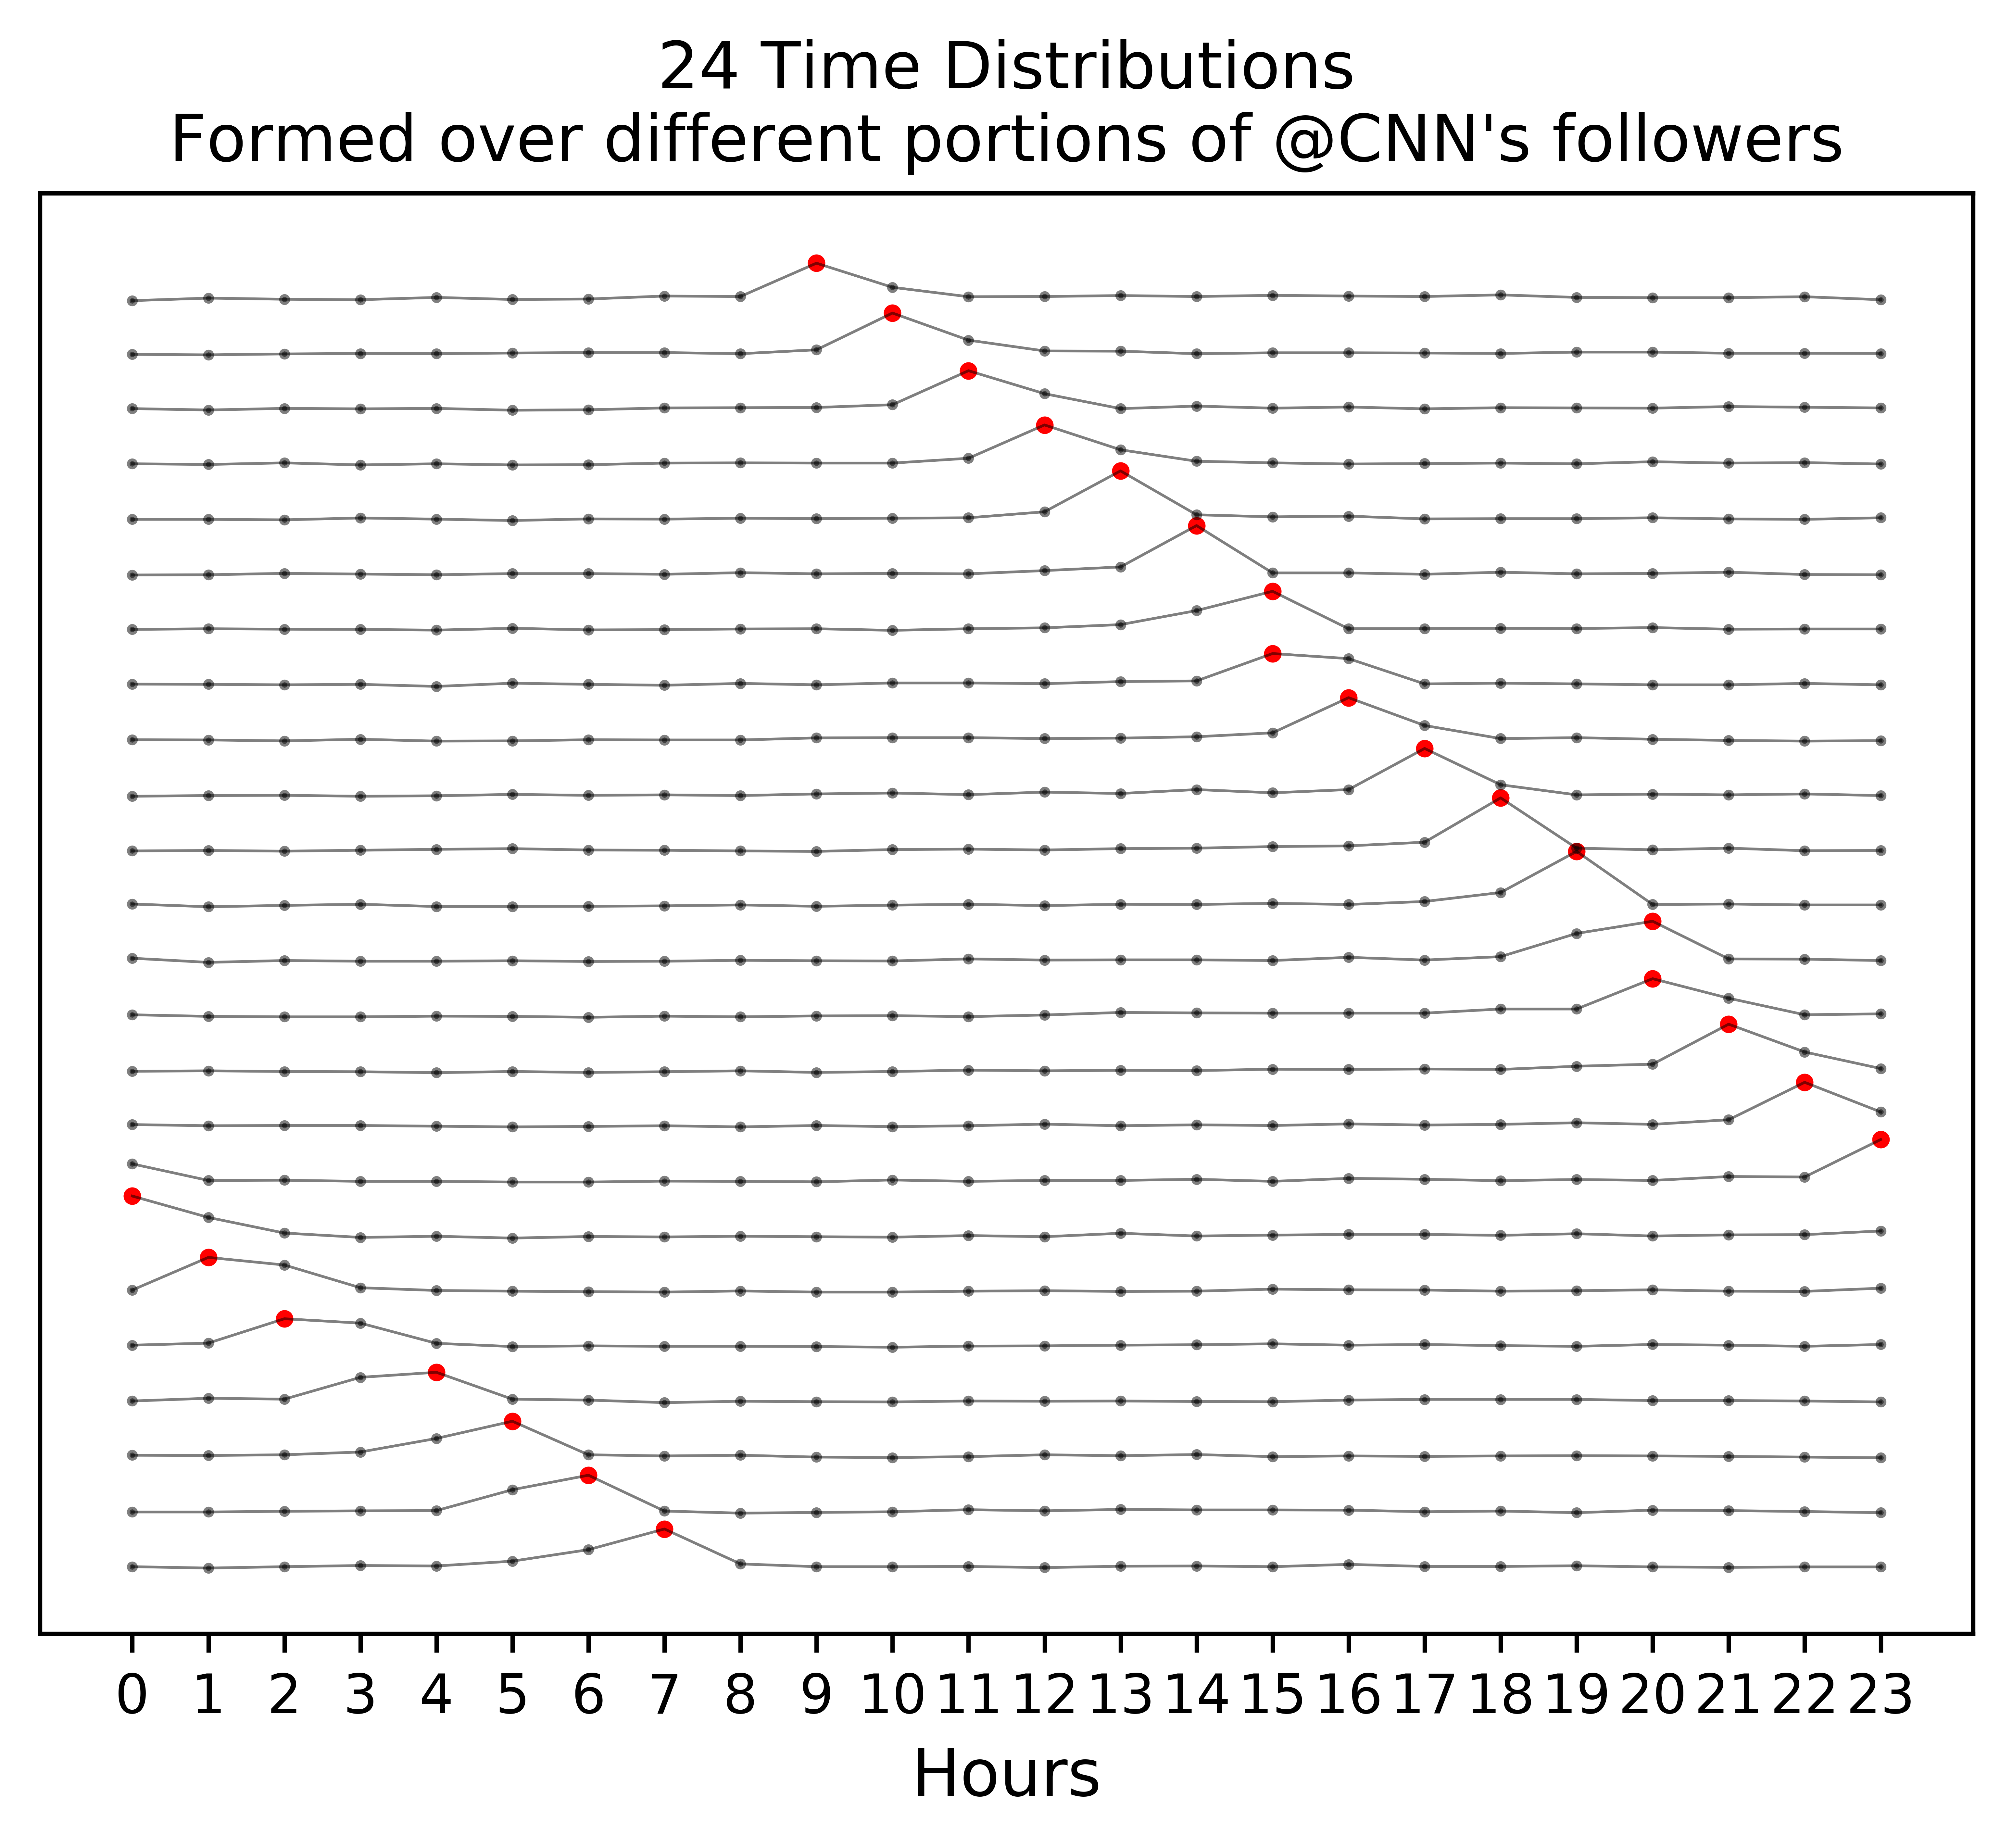
\includegraphics[width=5in]{Figures/Stackedcnn600.png}
\caption[Peak Analysis over Followers of @CNN]{24 time distributions where each time distribution formed from $n = 600$ followers of \emph{@CNN} for a total of $24 \times 600=14400$ followers. Distributions are plotted one above the other ($L_1, L_2, \ldots, L_{24}$). For each distribution the hour during which it peaks is highlighted in red. %Note the cyclical pattern observed by these peaks that in sequence cover all 24 hours.
}
\label{fig_3N}
\end{figure}

\subsubsection{Representing Cyclical Nature of Time}

\begin{figure}[!t]
\centering
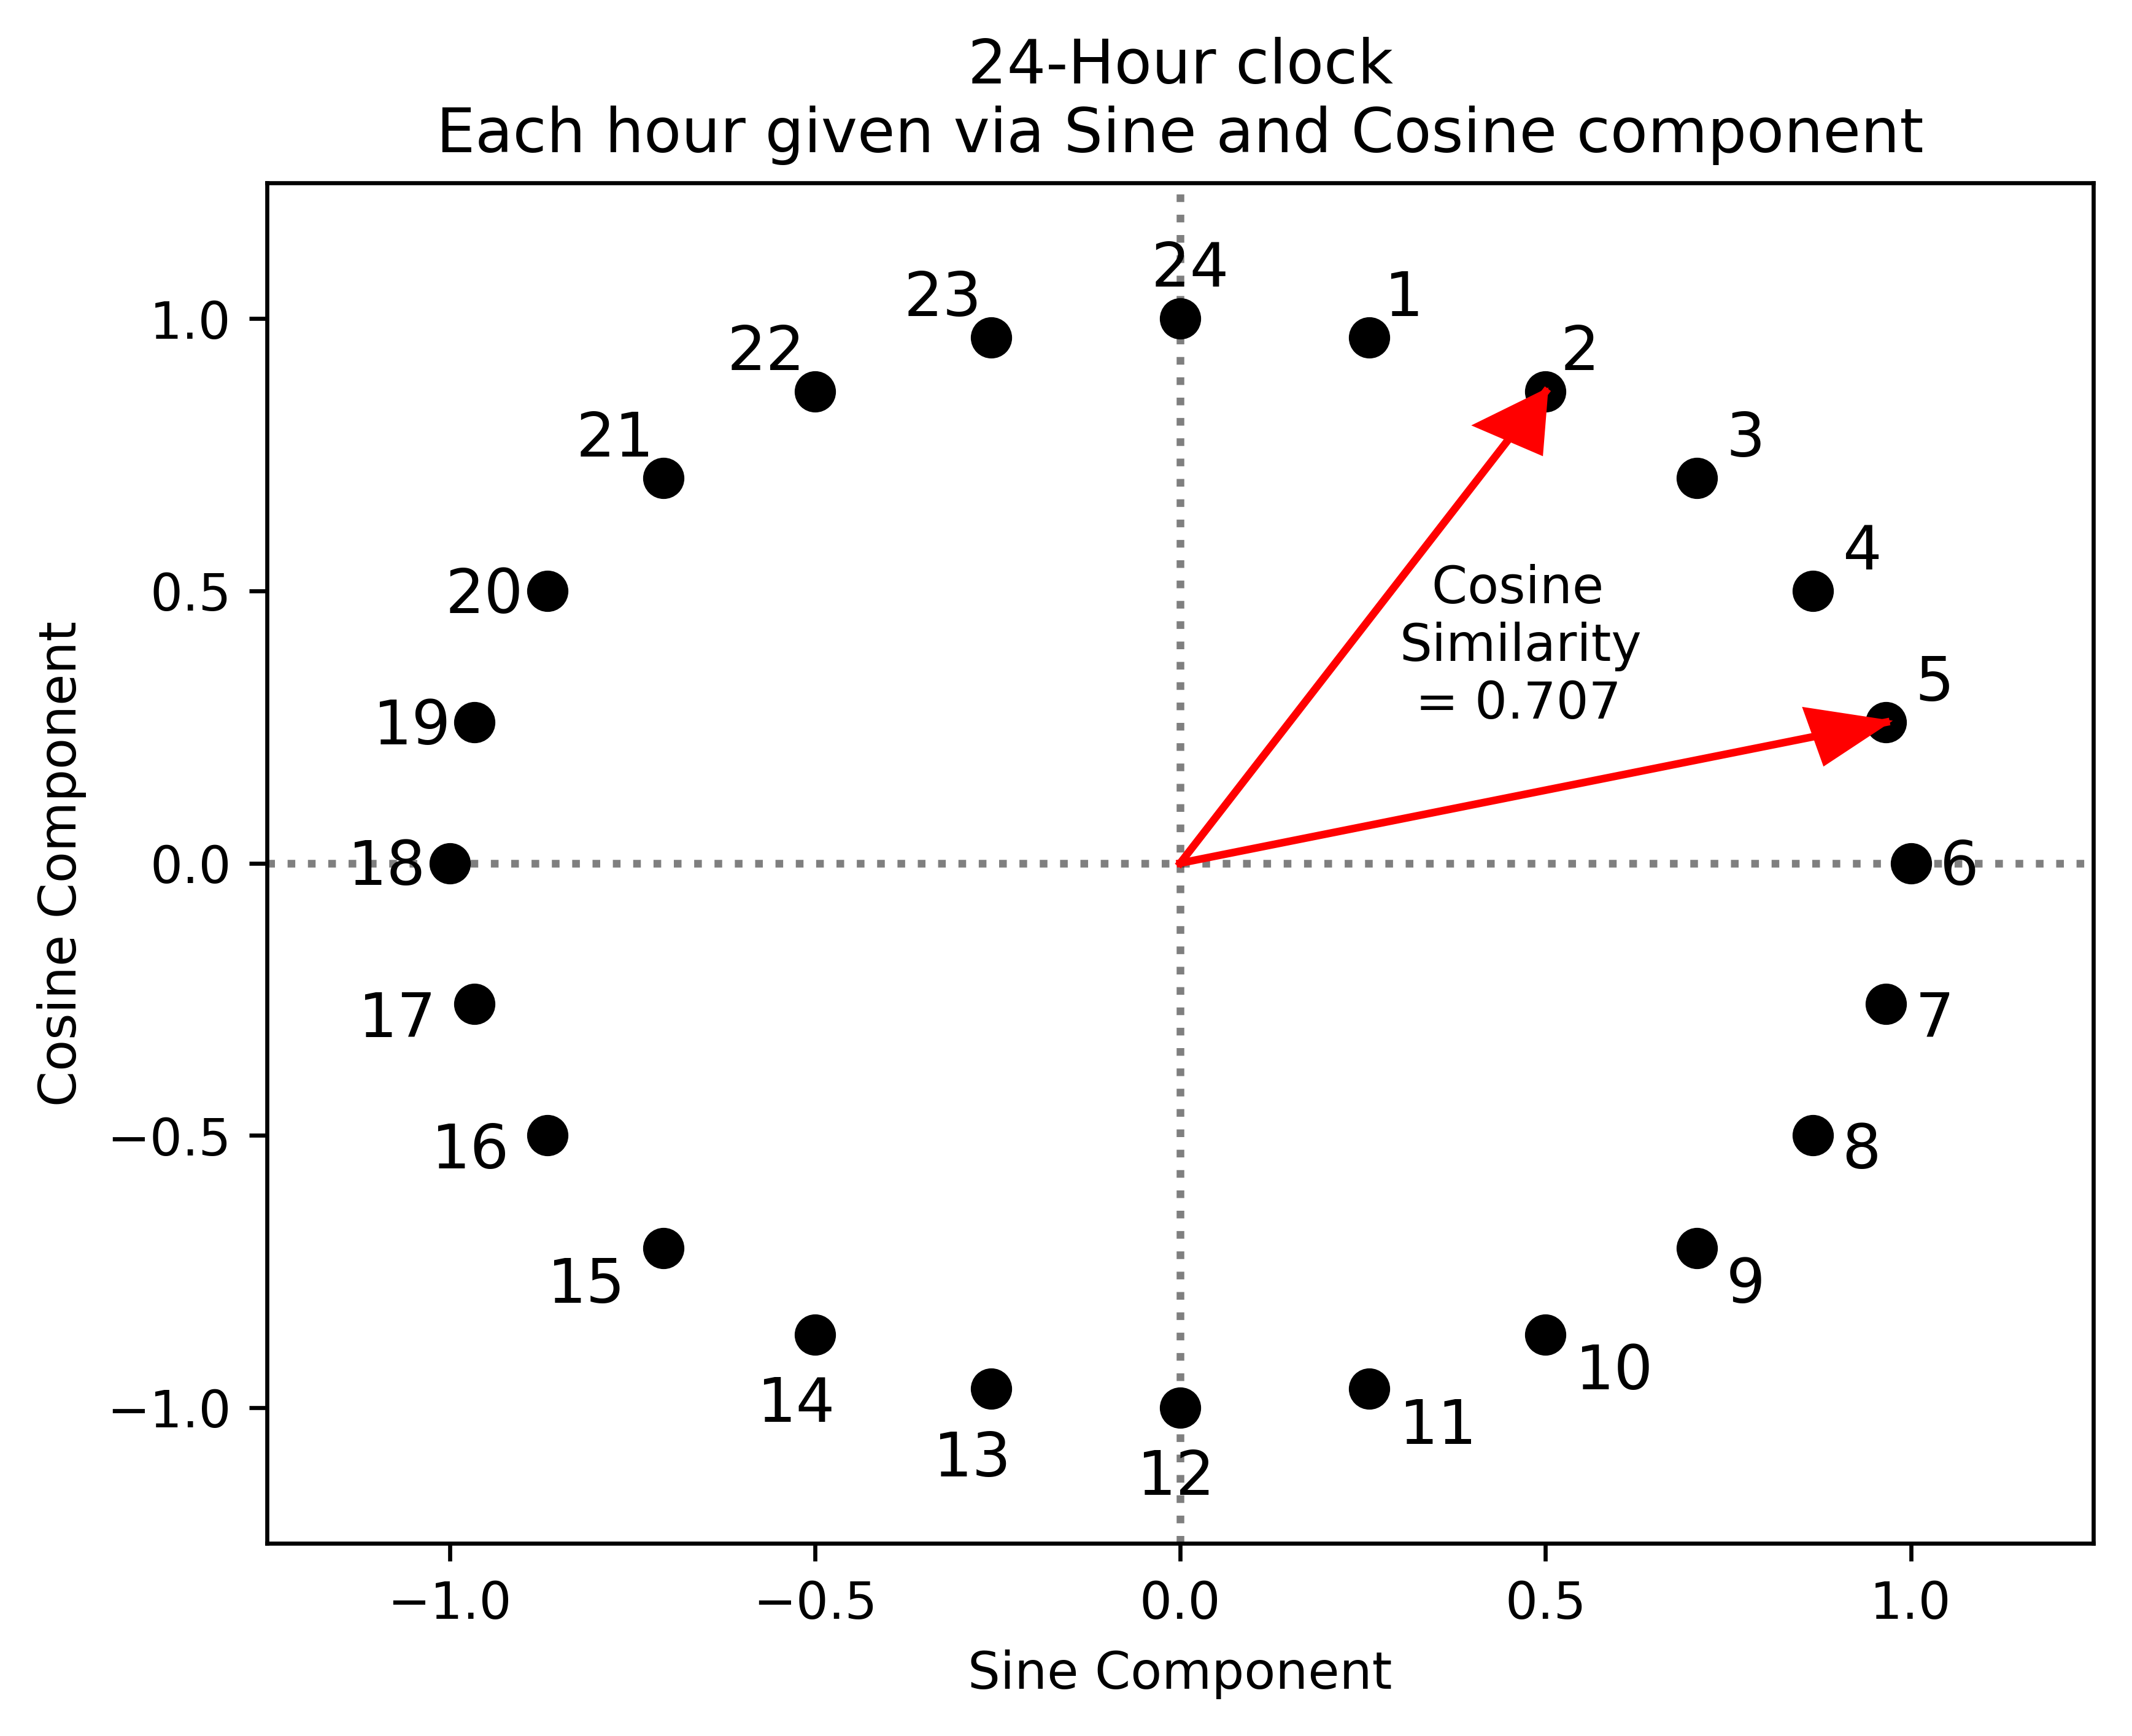
\includegraphics[width=.45\textwidth]{Figures/24HourClock.png}\hfill
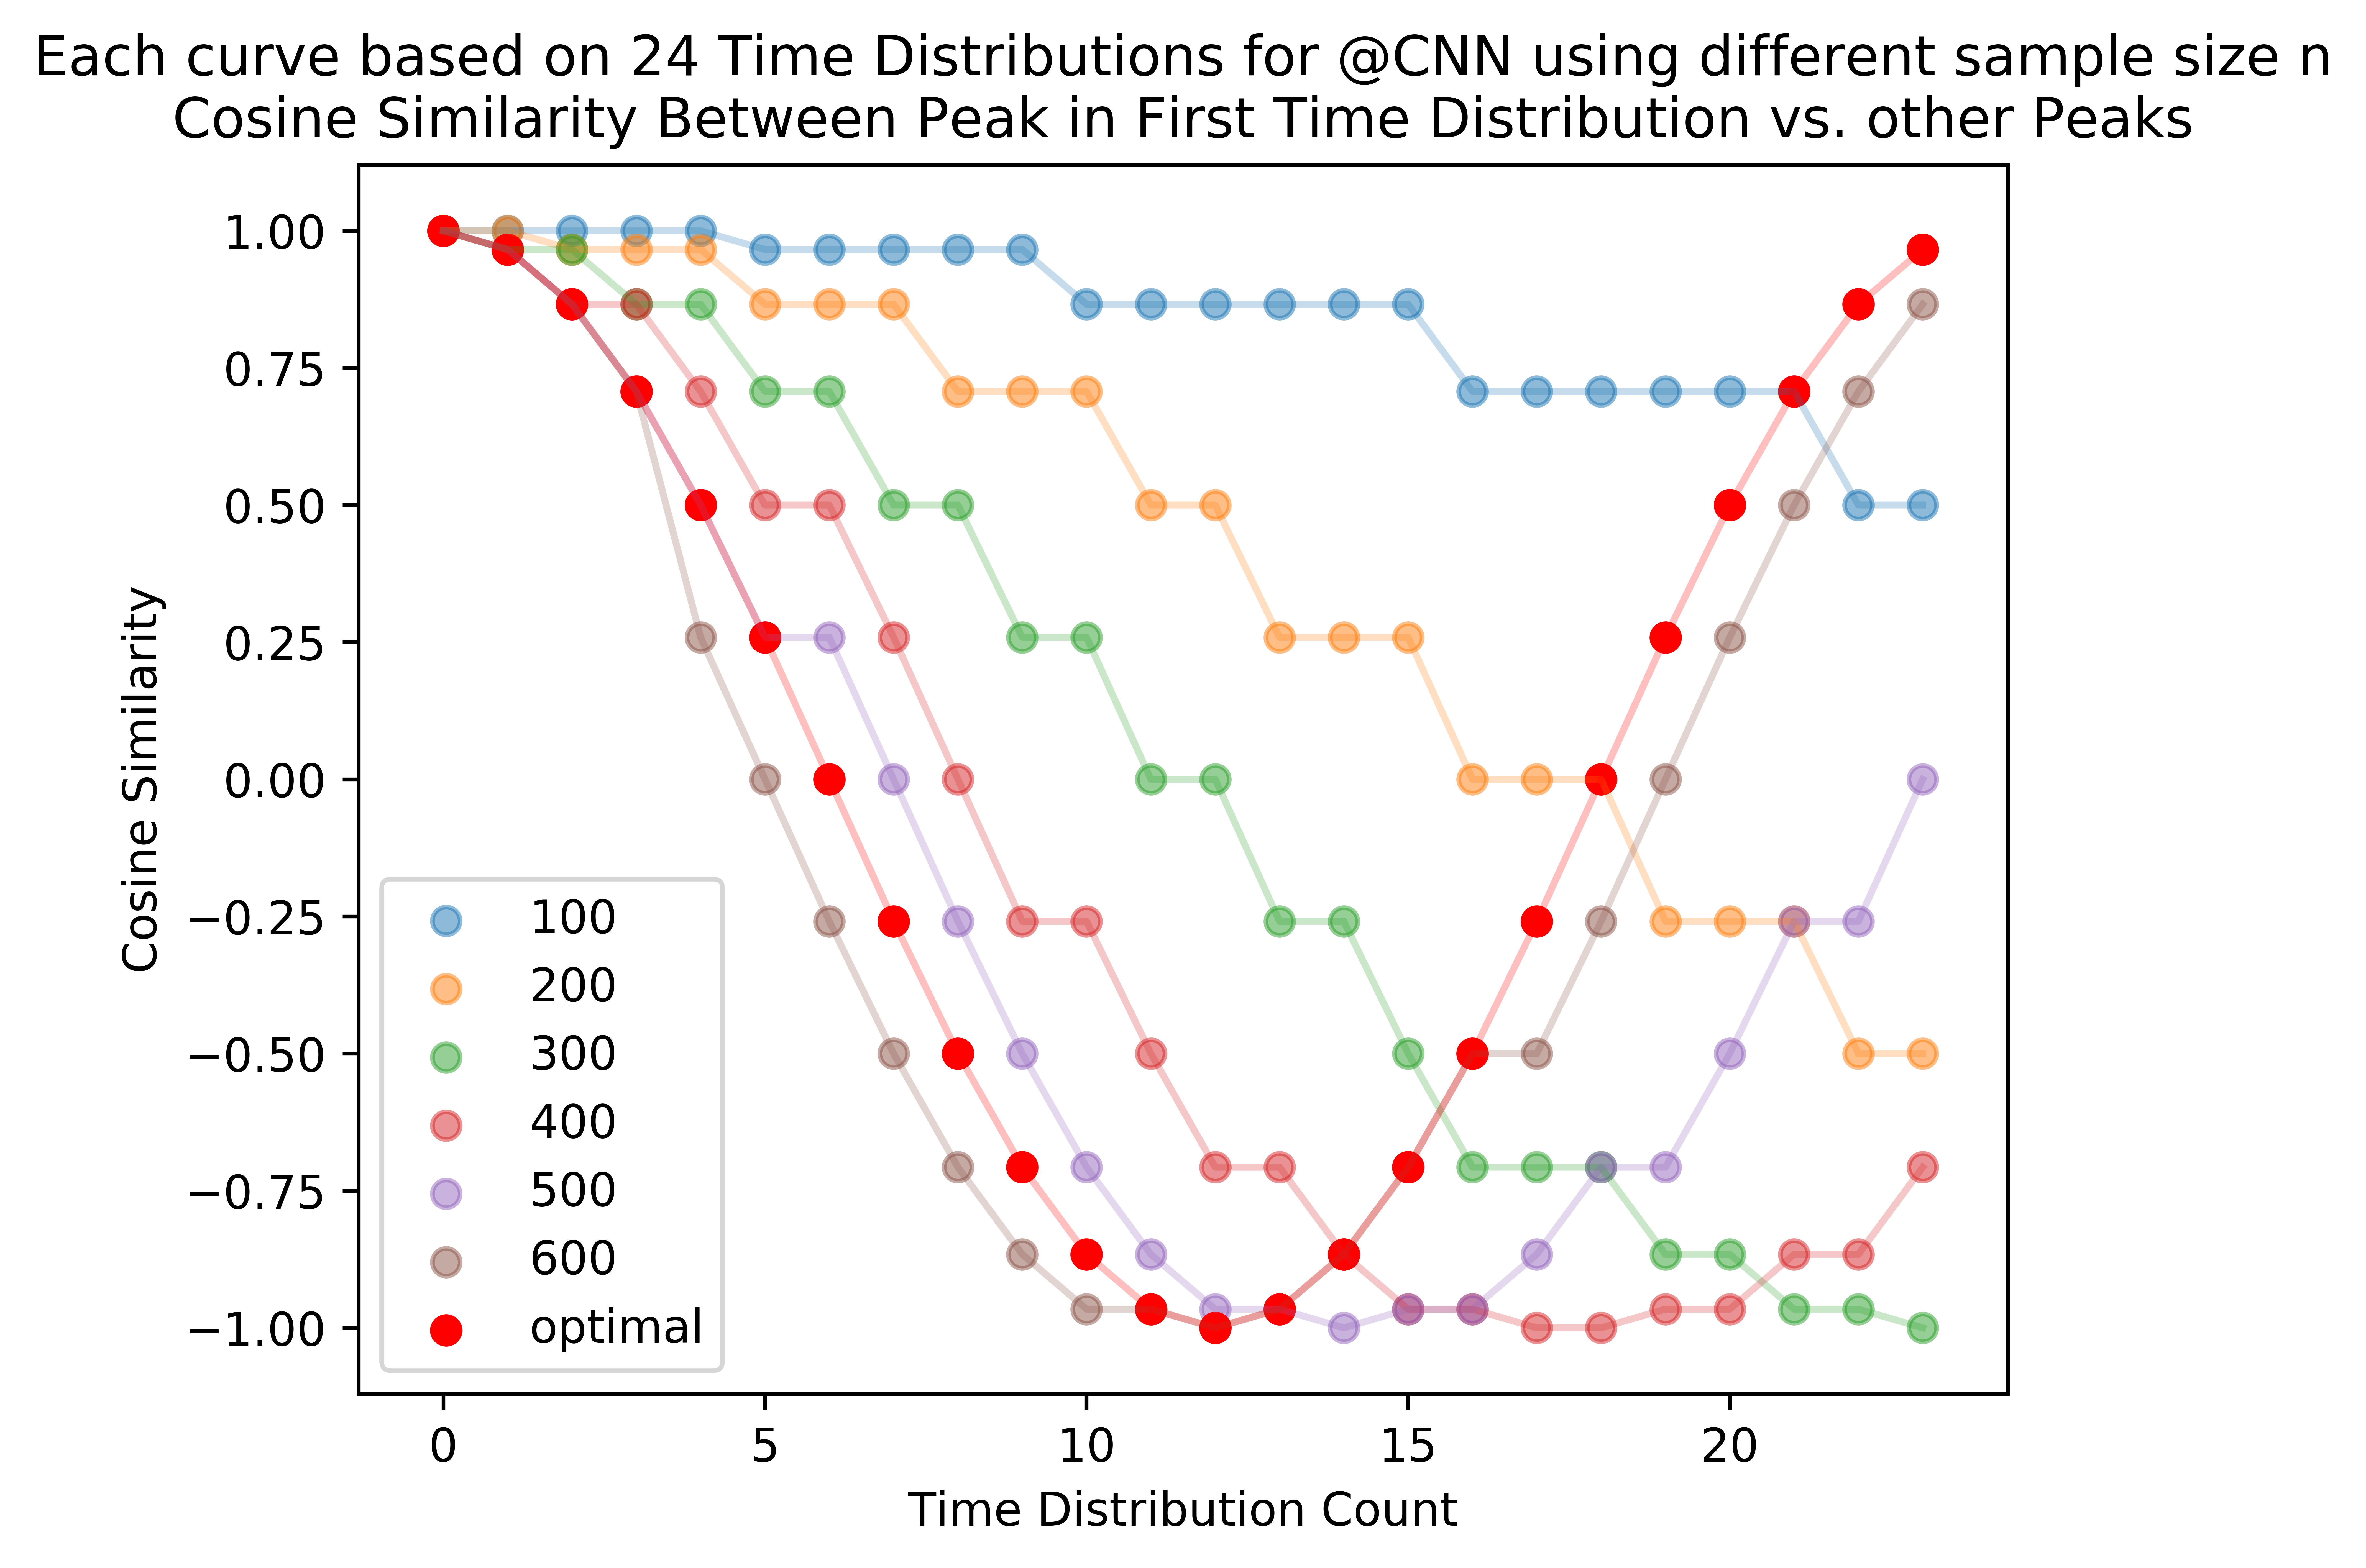
\includegraphics[width=.55\textwidth]{Figures/CosineDistance.png}
\caption[Cosine Similarity using 24-hour Clock]{\textbf{Left} --  24-hour clock; illustrates the computation of the cosine similarity between two hours. \textbf{Right} -- Each curve is computed using cosine similarity between the peak time in the first time distribution vs. itself and peak times over remaining 23 time distributions for various $n$ as described in the text (all graphs for \emph{@CNN}). The red curve is optimal in that the peaks are in the order of the hours on the clock. 
}
\label{fig_5N}
\end{figure}

In the 24-hour clock, shown in Fig. \ref{fig_5N}, each hour can be represented using sine and cosine values of the angle the hour-hand makes with the vertical straight line from the center to the 24\textsuperscript{th} hour. The angle for an hour $h$ in degrees is given as $\textstyle\frac{360 \times h}{24}$. For example,  the angle for 2 O'clock is $\textstyle\frac{360\times2}{24} = 30^o$  and 2 O'clock is represented as $(\sin 30^o, \cos 30^o)$ = (0.5, 0.866). Similarly 5 O'clock is expressed as $(\sin 75^o, \cos 75^o)$ = (0.965, 0.258). The cosine similarity between (0.5, 0.866) and (0.965, 0.258) is 0.707. If we plot the cosine similarities of (sine, cosine) representation of a specific hour A, with  (sine, cosine) representations of hours A, (A+1), (A+2), $\ldots,$ we obtain a smooth cosine curve (see red plot on the right of Fig. \ref{fig_5N}). The vector of the above cosine similarities is denoted as $V_1$ and is called the optimal vector.

Now consider the peak hour in each distribution of \emph{@CNN} in Fig. \ref{fig_3N}. If we compute and plot the vector $V_2$ of cosine similarities between (sine, cosine) representations of these hours with the representation of hour 7 (where the peak occurs in the first distribution), we obtain the brown curve in Fig. \ref{fig_5N}. Likewise, vectors of cosine similarities resulting from sample sizes given by $n$ = 100, 200, 300, 400, and 500 are shown. The similarity between $V_1$ and $V_2$ can be computed using $\rho$, the Pearson Correlation Coefficient. 

We are interested in the size of $n$ that results in temporal distributions that peak exactly one hour apart for all 24 hours (or as close to it as possible). For example, in Fig. \ref{fig_5N}, the curve associated with $n=600$ is closest to the ideal red curve. The key idea is to try different values of $n$ and calculate the associated $V_2$ vectors. The vector $V^*_2$ with the highest correlation against $V_1$ and associated  $n^*$ are obtained. The number of followers gained over 24 hours is predicted as $p_{24} = 24 \times n^*$. A formal description of the algorithm is provided below.
 


\subsubsection{The Algorithm} \label{algo-gain} Input to the algorithm is the list, $\mathcal{L}$, of an influencer's followers  and the precomputed optimal vector $V_1$.  Next,  $n$ is chosen from a minimum of 10 to a maximum of $\lfloor\frac{|L_1|}{24}\rfloor$. For each $n$, 24 time distributions are generated and from each, the hour during which the time distribution peaks is recorded. $V_2$ is generated using cosine similarity between the %first peak hour vs. the sequence of other peak hours.
peak hour in first time distribution vs. peaks across all 24 time distributions.
$V_1$ and $V_2$ are compared using the Pearson Correlation Coefficient $\rho$. The sample size $n^*$ that resulted in the highest correlation coefficient is returned. The predicted 24 hour followers turn over, $p_{24}$, is given as $ 24 \times n^*$.

{\fontfamily{pcr}\selectfont
\begin{tabbing}
\textbf{Al}\=\textbf{go}\=\textbf{ri}\=\textbf{th}\=\textbf{m 1}\=: \textit{infer24HF(L1)}:\\
\> \textbf{Input}: List L1 of follower creation times; \\
\> \textbf{Output}: Predicted 24 Hour Follower Gain, associated\\
\> Pearson Correlation, and number of unique peaks;\\
\> bestN, maxP, maxH = 0, 0, 0;\\
\> V1 = vector of cosine similarities between\\
\> \> \> hour 0 and hours [0, 1, 2, ..., 23];\\
\> for n in [10, 15, ..., |L1|/24]:\\ 
\> \> Split first 24*n elements of L1 into 24 bins of size n;\\
\> \> Record the hour with most elements for each of 24 bins;\\ 
\> \> V2 = vector of cosine similarities between\\
\> \> \> \> hour in bin 1 and hours in each bin;\\
\> \> P = Pearson Correlation between V1 and V2;\\
\> \> if P $>$ maxP:\\
\> \> \> bestN = n;\\
\> \> \> maxP = P;\\
\> \> \> maxH = number of unique peaks across bins;\\
\> Return bestN*24, maxP, maxH; \\ 
end 
\end{tabbing}
}

\subsection{Evaluation}

For each influencer in $D_{600}$, we compute $p_{24}$ and compare it to known follower gain $a_{24}$, using the comparison measure \textit{diff($p_{24}$, $a_{24}$)} = max($p_{24}/a_{24}, a_{24}/p_{24}$)-1.

Fig. \ref{fig_6N} shows the scatter plot of $p_{24}$ versus $a_{24}$ for all influencers in $D_{600}$. The scatter plot is color-coded: green dots represent  influencers with \textit{diff}$\le 0.25$, and red dots represent large differences with \textit{diff}$>1.0$. The Pearson correlation coefficient between  $p_{24}$  and $a_{24}$ vectors is $\rho =0.967$, a high value that shows that the proposed  method makes  accurate predictions. %For example, for  \emph{@CNN} $n^* = 625$ and the  predicted gain is  $ (n*24 = 15000)$;  whereas the actual gain  is 15617.

\begin{figure}[!t]
\centering
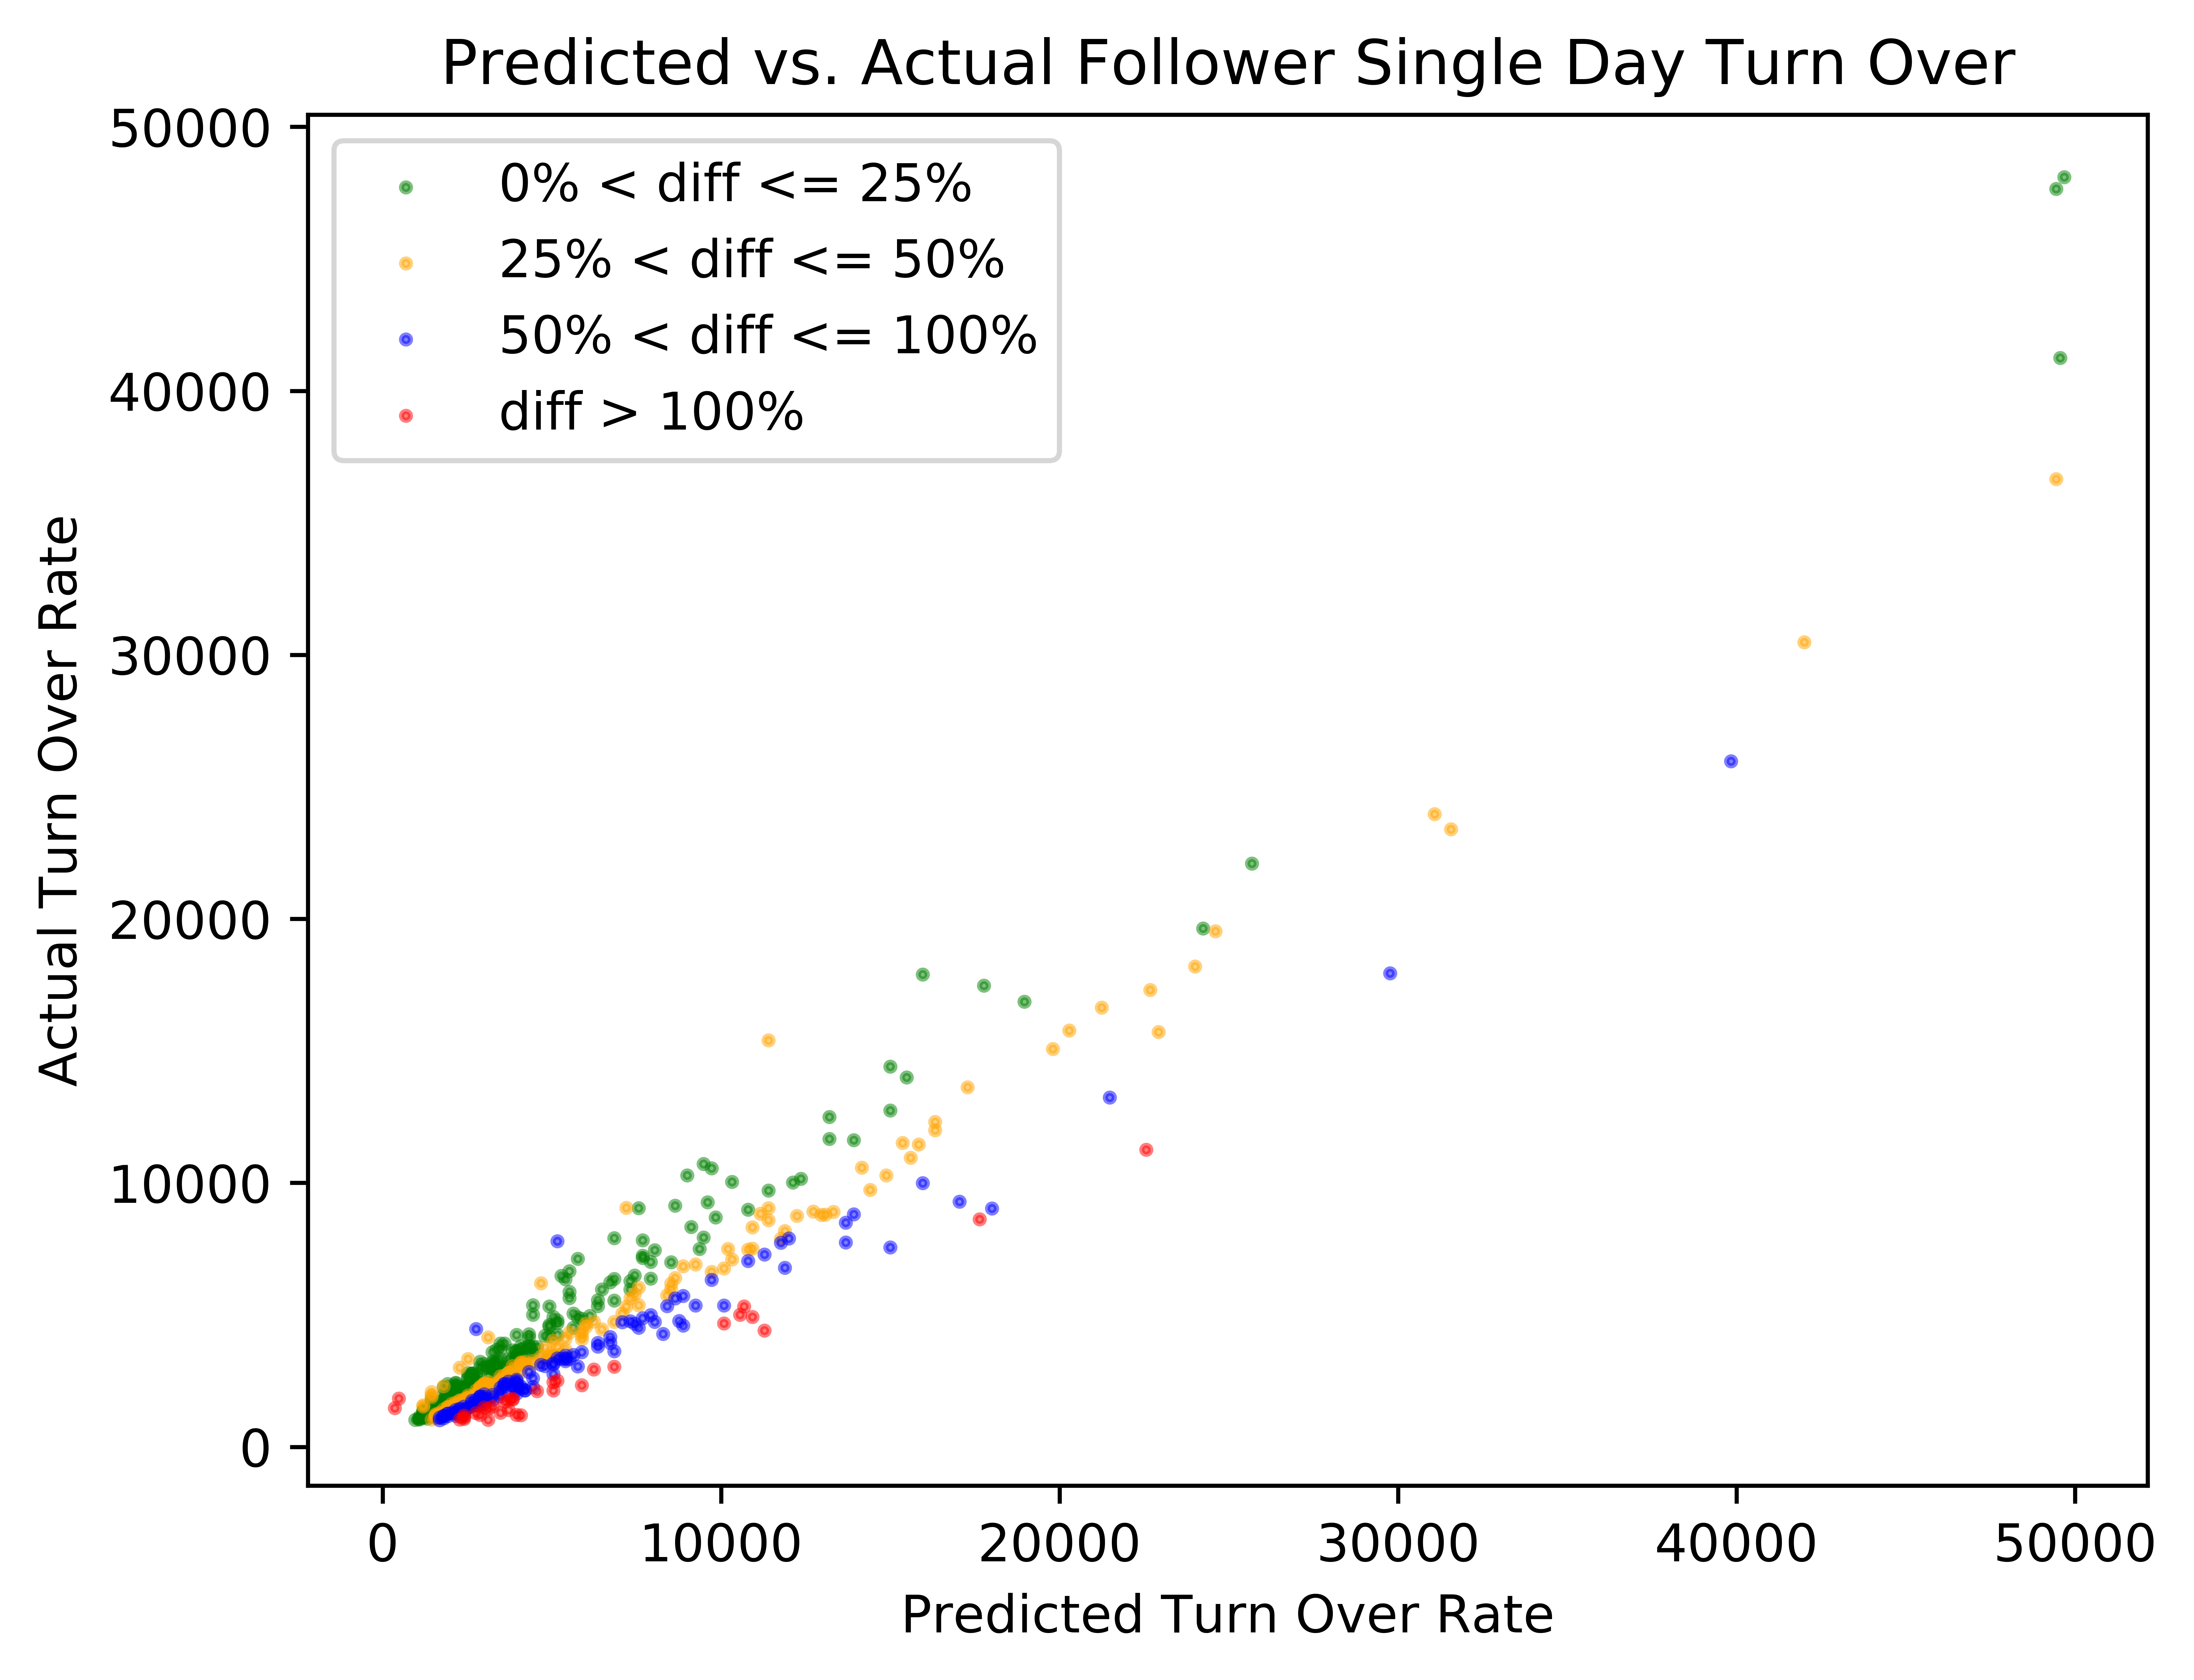
\includegraphics[width=4.5in]{Figures/percturnRate.png}
 \caption[Scatter plot of Inferred vs. Actual daily follower gain]{Scatter plot of Inferred vs. Actual number of followers gained by 600 influencers over a 24-hour time period (Pearson correlation coefficient = 0.967);  238 points (green) differ by  $<25$\%, 195 points (orange) differ by $<50$\%, 126 points (blue) differ by  $<100$\%, and 41 points (red) differ by $\geq100\%$.}
\label{fig_6N}
\end{figure}

We compare our algorithm against two baselines. Meeder et al. [\ref{appendix:5.15}] provide a method for estimating when a user had followed the influencer. Given a list of followers' creation times $L_1$ for influencer $i$, the follow time for a follower at index $j$ is approximated by max($L_1[j:]$) (max gives the most recent creation time at indices greater than or equal to $j$). For our problem we are interested in the number of followers gained over 24 hours so that the datetime max($L_1[j:]$) is as close to the datetime that is 24 hours before the follower collection took place (given by $\mbox{Followers}_t(i)$ minus 24 hours). Effectively we are trying to utilize the method proposed by Meeder to estimate the index $j$ that would satisfy this requirement. The method should work for those influencers that are likely to be followed by brand new users immediately after their account creation. 

%We implemented two baselines based on the method proposed by Meeder et al. [\ref{appendix:5.15}]. 
$\mbox{Followers}_t(i)$ gives time $t$ for influencer $i$'s followers collection.  %Let $\mathcal{L}_M$ be the list such that 
Let $\mathcal{L}_M[j] =$
$(t-\mbox{ creation time of the }   j^{th}  \mbox{ follower of the influencer}$, for $j = 0, 1,  \ldots)$. 
%The first prediction of the influencer's follower gain is obtained as follows:

\subsubsection{Baseline 1:} Traverse the list, $\mathcal{L}_M$, in reverse order and find the first index $j$, such that $\mathcal{L}_M[j] \leq \mbox{ 24 hours}$. If such a $j$ exists, then return $j+1$, denoted as $p_{24}^{(B1)}$; else return $|\mathcal{L}_M|$. 

\subsubsection{Baseline 2:} For each $j$, such that $\mathcal{L}_M[j] \geq \mbox{ 24 hours}$ calculate $\frac{\mathcal{L}_M[j]}{j+1}$; Find the minimum ratio, which will approximate the average number of seconds that elapse per new follower; Return $p_{24}^{(B2)} =$ $\frac{86400}{ratio}$ (since there are 86400  seconds in 24 hours).

As before, we can calculate the correlation coefficient between the vectors of $p_{24}^{(B1)}$ and $a_{24}$ and between $p_{24}^{(B2)}$ and $a_{24}$ over all influencers. In addition, median error and MSE can be computed, where diff(predictions, $a_{24}$) is the error that is to be minimized. Table \ref{table_24HEval} shows how our approach  compares against baseline predictions based on these measures. 
%It can be seen that a
Correlation values of all three approaches are high, with slightly better values obtained by our approach.
In terms of median error and MSE,
 our approach performs much better than the baselines.
%perform well , but our method performs slightly better in all three measures. 
%Given this performance we also recommend utilizing the second baseline as an additional check against our method. 
\begin{table}[htbp]
\small
\caption{Performance of three algorithms to predict influencers' gains}
\label{table_24HEval}
\centering
\begin{tabular}{|c|c|c|c|}
\hline
\bfseries Approach & \bfseries Correlation & \bfseries Median Error & \bfseries MSE\\
\hline
Baseline 1 ($p_{24}^{(B1)}$)  & 0.962 & 0.620 & 0.665\\
\hline
Baseline 2 ($p_{24}^{(B2)}$)   & 0.964 & 0.541 & 0.510\\
\hline
Our  & 0.967 & 0.298 & 0.252\\
\hline
\end{tabular}
\end{table}

%\subsection{Rationale for improved performance} %Why the Algorithm works
\subsection{Rationale for Proposed Algorithm and its Limitations} %Why the Algorithm works
If we consider a group of users that %have performed an action
acted during a specific hour $h$ (such as posting a message or following another), then we are likely to observe a maximum near that same hour in their creation time distribution. This behavior has been confirmed, as discussed below, by analyzing time distribution for users grouped using the time that they have posted a message.

We utilize the dataset  $D_{mess}$. We take all messages that contain a specific token. For example, for token `@youtube' there were 13704 messages. Next, we separate the messages (containing that token) by the hour of message creation time. In this way, 24 groups of users are formed where each user group is known to have been active during a specific hour (the hour during which the message was generated). For each user group, we construct the creation time distribution. 

Fig. \ref{fig_Explanation}(a) shows a heat map for the 24 time distributions generated for token `@youtube'. Notice that a global concept `@youtube' will have a pattern down the diagonal like an Identity Matrix (`@youtube' considered global because $c_2<0.001$); the same analysis was performed using stopwords such as `the' and `you' and they also observe this pattern. The pattern is due to a unimodal distribution that peaks near the same hour as the hour during which the users were most active in generating the messages. Intuitively if a person had the time for creating their Twitter account in the morning then this person is likely to be active on the Twitter platform during the same morning hours in the future (there is thus a correlation between the creation times and activity times).

\begin{figure*}[htp]
   \subfloat[Messages with `@youtube']{\label{fig_Explanationa}
      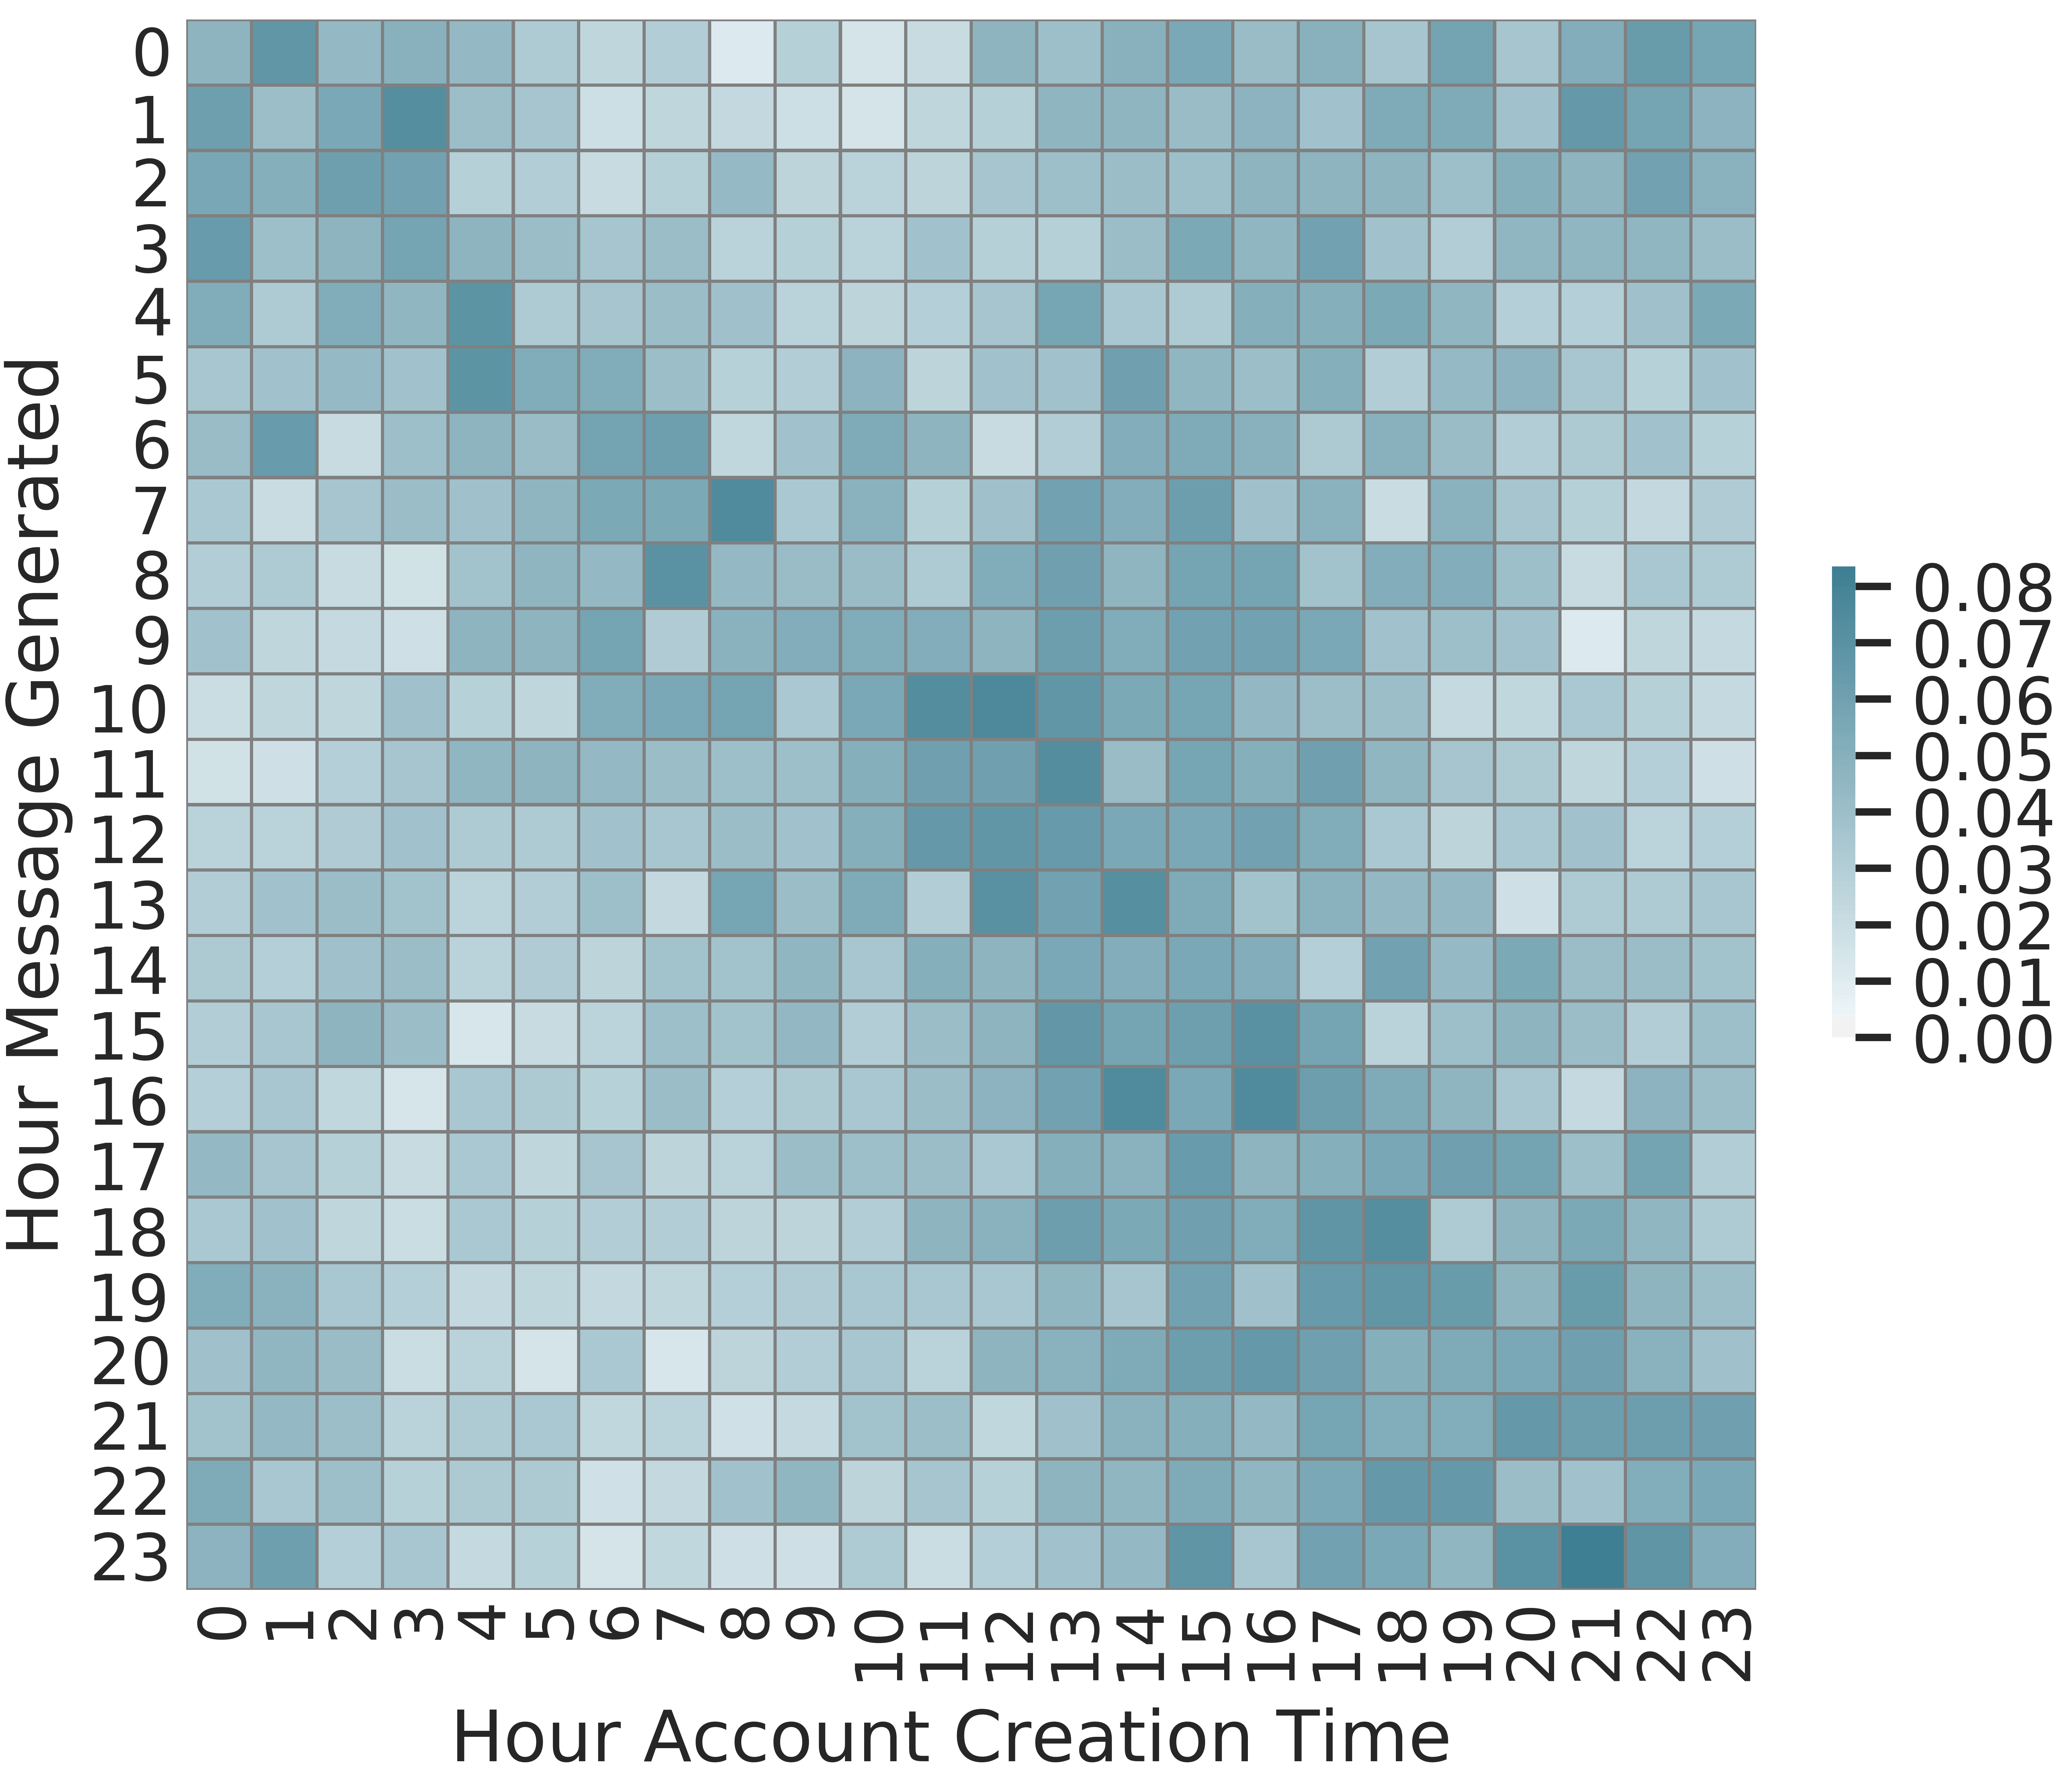
\includegraphics[width=.52\textwidth]{Figures/StackedDist@youtubeHeatmap2.png}}
   %\hspace*{\fill}   % maximize separation between the subfigures
   \subfloat[Messages with `trump']{\label{fig_Explanationb}
      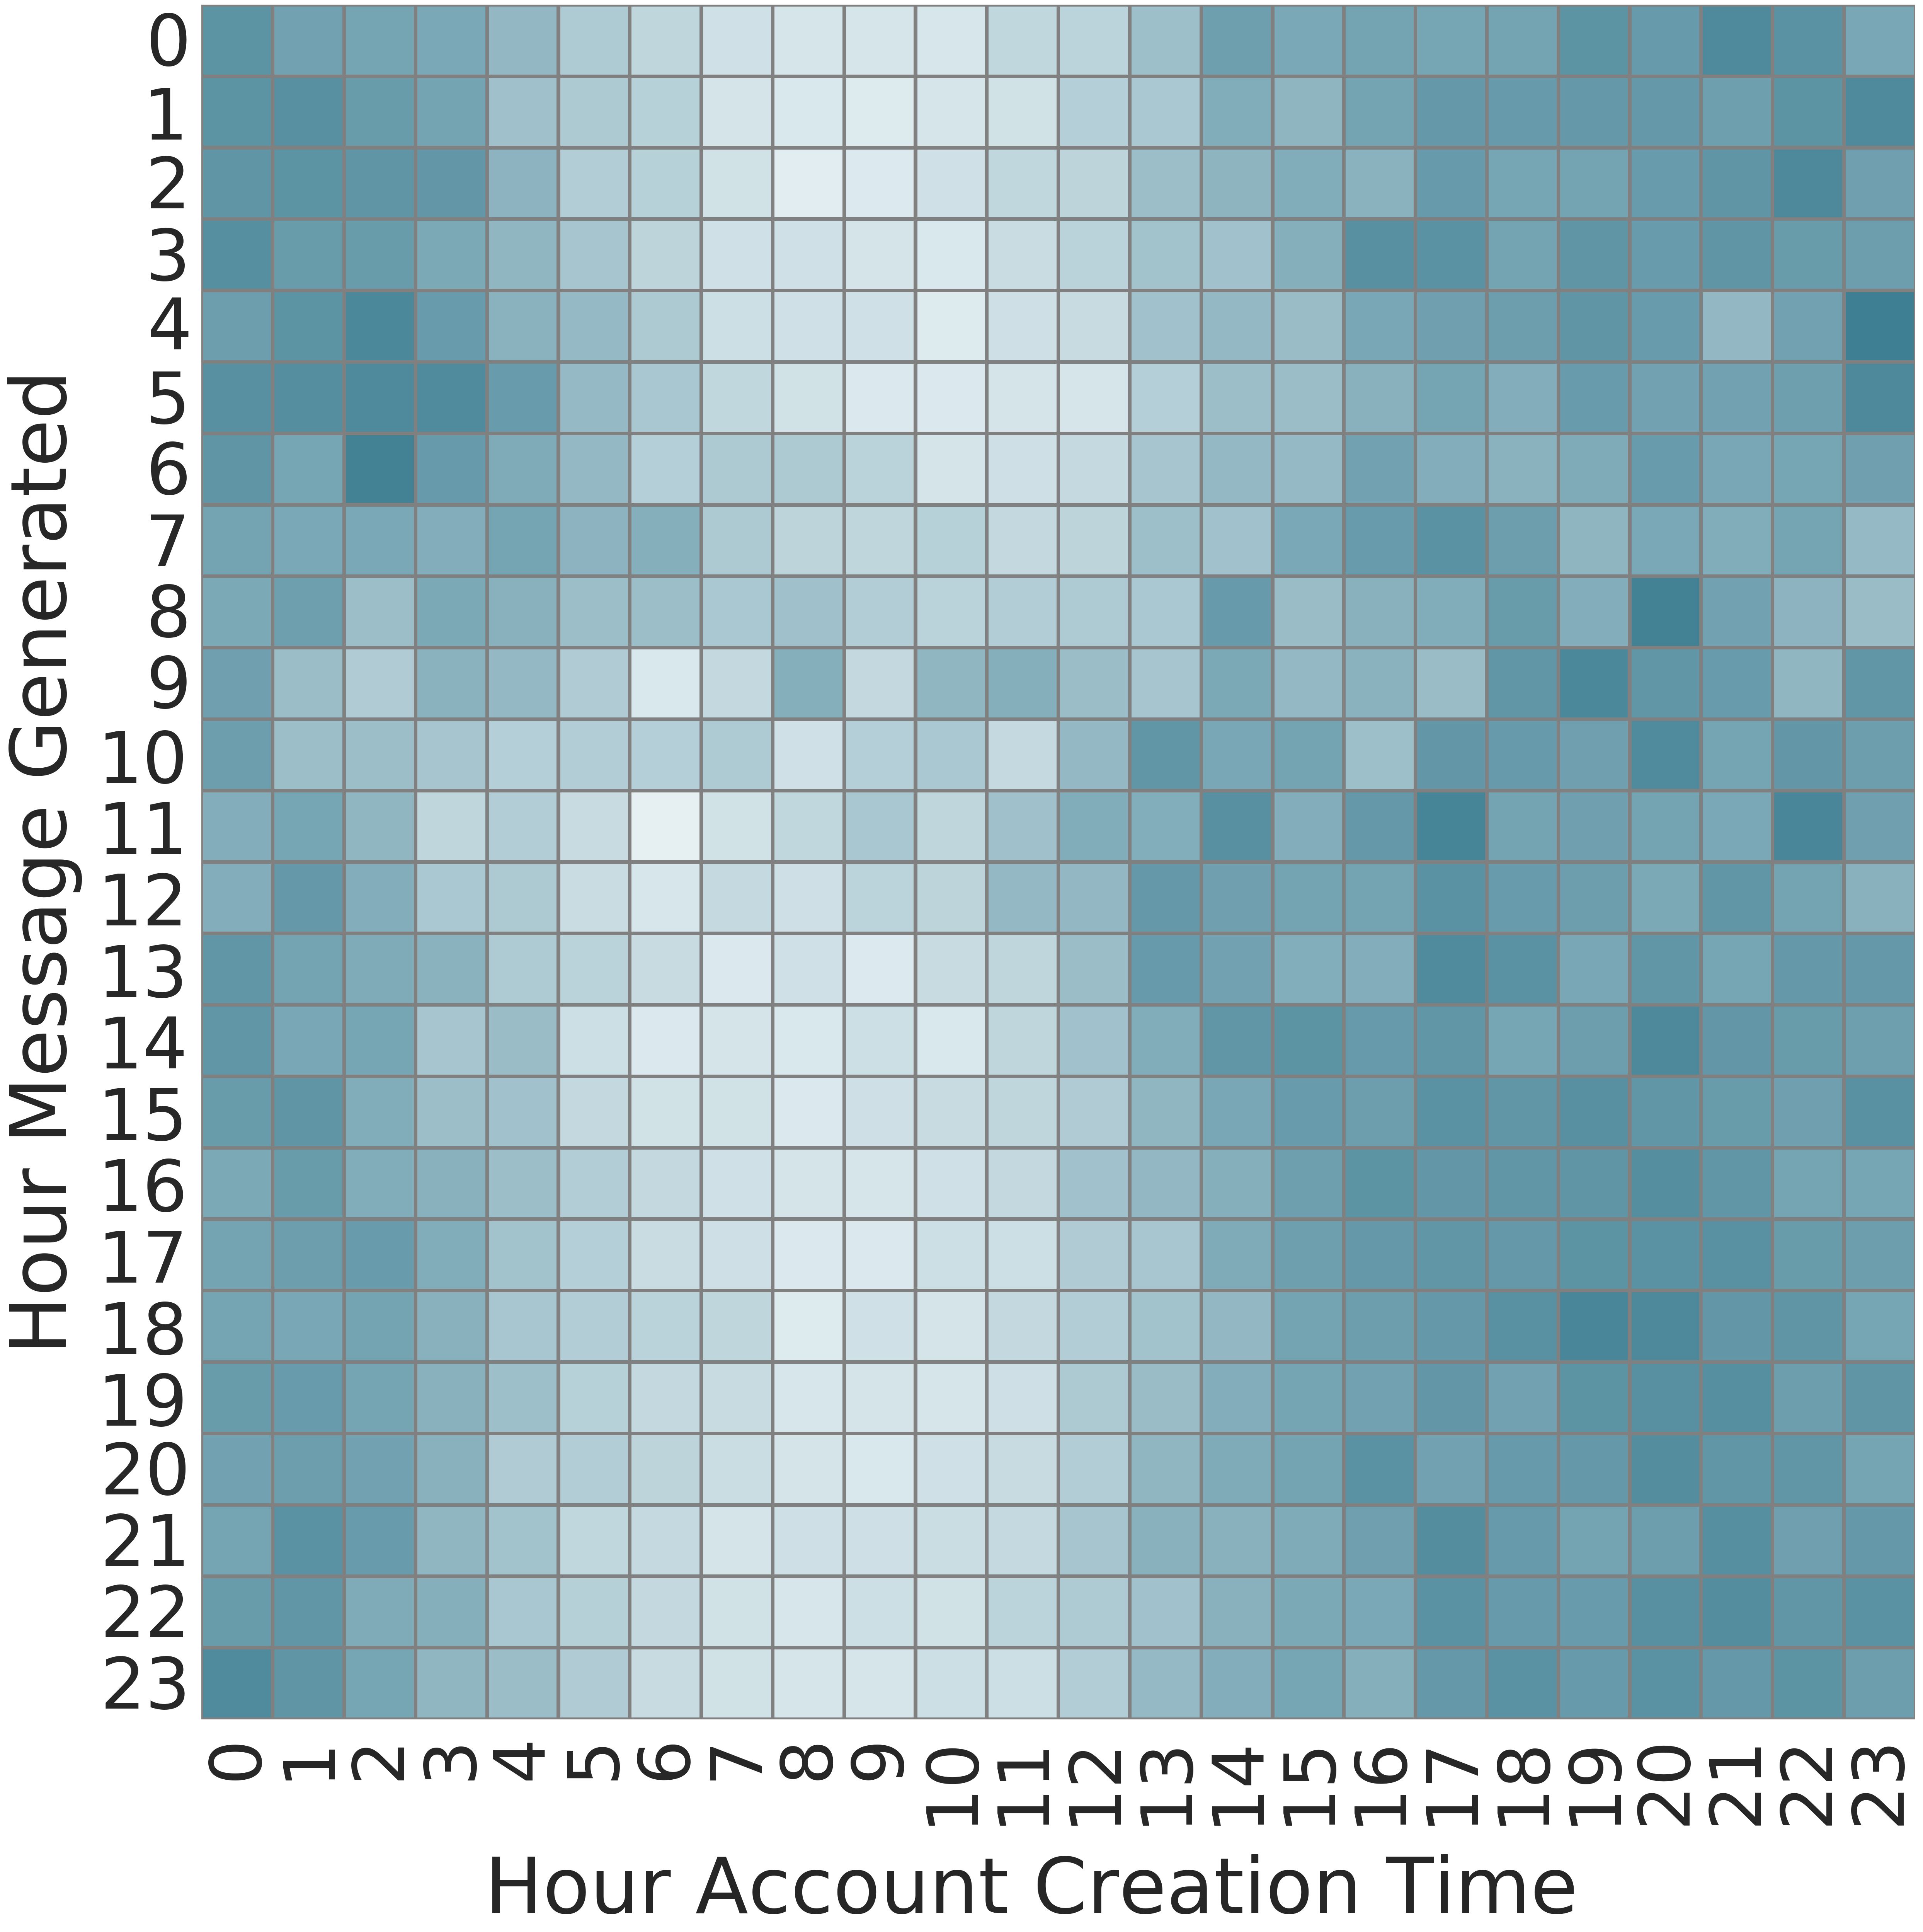
\includegraphics[width=.45\textwidth]{Figures/StackedDisttrumpHeatmap2.png}}
   \caption[Peak Analysis over Message Traffic]{Heat maps showing 24 time-distributions from users’ creation times where users are binned by the hour that they generated messages containing tokens: (a) `@youtube' 
   (global) and (b) `trump' (local). For a global token like `@youtube' we see that if a user was active in posting a message during hour $h$, then the user was likely to have created their account near the same hour $h$. For token `trump' a sleep cycle is observed (period of inactivity hours 5-11).} \label{fig_Explanation}
\end{figure*}

The distinction between global and local influencers is illustrated by comparing Fig. \ref{fig_Explanation}(a) vs. Fig. \ref{fig_Explanation}(b). Fig. \ref{fig_Explanation}(b) focuses on a more localized token 'trump' that clearly has a period of inactivity, a sleep cycle, during hours 5-11 (token has $c_2 > 0.001$ and during the collection period it was heavily discussed in the Americas). 

The concepts observed over message analysis apply to studying the influencer's followers. We do not know when a user followed an influencer, but because the followers are in sequence of follow time this indicates which followers must have followed earlier on. Algorithm 1 attempts to find a batch of followers of size $n$ that results in a unimodal distribution, which indicates that the followers are likely to have followed the influencer during the same hour as their account creation. When 24 batches, of size $n$, each peak during a different hour in sequence, it gives confidence that the follower gain around the 24-hour time period has been accurately identified (as has been illustrated in Fig. \ref{fig_3N} for followers of \emph{@CNN} and like the Identity Matrix in Fig. \ref{fig_Explanation}(a)).

Algorithm 1, for this reason, is well suited for global influencers that are gaining followers around the clock. In contrast, the heat maps for localized influencers show no strong peaks during some hours of the day. The approach, presented above, also cannot be relied upon for influencers that are gaining no more than 50 followers a day, because the average hourly batch will be too small to generate a meaningful time distribution. 

There will be periods during which an influencer gains no followers and even loses followers. We can reason only about followers that the influencer currently has, i.e., we cannot know which followers an influencer might have had in the past. If the influencer has lost many original followers, then the signal in the data will be obscured by considerable noise; $\rho$ will be small since the peaks will not cover all hours, and the order might not be perfect. Hence we have chosen to focus on influencers that have a large stable following and that are continuing to increase their follower base. It is preferable to pay close attention to $\rho$ and to stop making inferences after $\rho$ goes below some threshold. It is also recommended to compare the modified baseline based on Meeder et al. [\ref{appendix:5.15}] as an additional check against our method.

\subsection{Studying the Evolution of Popularity}

To study an influencer's evolution of popularity we need to find  how many followers the influencer has gained over multiple days. In an earlier subsection, we have shown that we can estimate an influencer's follower gain over past 24 hours. 
The same technique can be repeatedly applied to study the gains  over a longer time span. 

To understand the evolution of an influencer's popularity, we first find its followers' creation time list, $L_t$, obtained at time $t$. Unlike the list in the previous section that contained only 50K followers, this list consists of all available followers of the influencer. 

Say we have an influencer with 10 million followers. We could send the whole list to Algorithm 1, but it is not reasonable for the influencer to have gained 10 million followers in 1 day, and so to reduce computation we send a smaller more reasonable list. The feature $wSize$ sets the threshold for the maximum number of followers to send to Algorithm 1 (this threshold can be increased or decreased based on influencer's popularity).
 
 Using the first $wSize$ followers between indices [0, $wSize -1$] of $L_t$, Algorithm 1 calculates the number of followers gained %over one day (
 between $t$ and $t-1$, denoted as $p_{24}^t$. The next $wSize$ followers between indices: [$p_{24}^{t}$, $wSize + p_{24}^{t}-1$] will calculate $p_{24}^{t-1}$ (gain between $t-1$ and $t-2$). The next $wSize$ followers between indices: [$p_{24}^{t}+p_{24}^{t-1}$, $wSize + p_{24}^t+p_{24}^{t-1} -1$] will calculate $p_{24}^{t-2}$ (gain between $t-2$ and $t-3$). The daily gains returned as list: [$p_{24}^t$, $p_{24}^{t-1}$, $p_{24}^{t-2}$, ....] successively going backward in time.
 
 Using this approach with $wSize=50000$, Table \ref{table_5N} illustrates the number of followers gained in the last 10 days by two examples of qualitatively different kinds of influencers: \emph{@MrBeastYT} and \emph{@NPR}. The table also contains the associated correlation values (suggesting the degree of confidence), and the maximum number of unique hours captured by the peaks for each calculation from Algorithm 1. We observe that \emph{@MrBeastYT} consistently adds more followers %(per single period or cycle in chart) 
 than \emph{@NPR}. \emph{@MrBeastYT} also has higher unique hours and higher correlation, suggesting greater confidence in these predictions. This is reasonable since a more popular influencer will have more hourly followers, and consequently, the time distribution will be formed using more data points.
 
\begin{table}[htbp]
\small
\caption[Inferring Daily Follower Gains over 10 days]{Comparison of numbers of followers gained 
($p\textsubscript{24}\textsuperscript{t-d}$)
over each of 10 days by two influencers, along with correlation values maxP and the number of hours maxH spanned by the followers in each 24-hour period}
\label{table_5N}
\centering
\begin{tabular}{|c|c|c|c|c|c|c|}
\multicolumn{1}{c}{}  & \multicolumn{3}{c}{\bfseries \emph{@MrBeastYT}} & \multicolumn{3}{c}{\bfseries \emph{@NPR}}\\
\hline
\bfseries period t-d & \bfseries p\textsubscript{24}\textsuperscript{t-d} & \bfseries maxP & \bfseries maxH & \bfseries \bfseries p\textsubscript{24}\textsuperscript{t-d} & \bfseries maxP & \bfseries maxH\\
\hline
t-1 & 12480 & 0.989 & 20 & 1680 & 0.759 & 18\\
\hline
t-2 & 12120 & 0.993 & 21 & 1560 & 0.944 & 18\\
\hline
t-3 & 14400 & 0.98 & 22 & 1440 & 0.678 & 20\\
\hline
t-4 & 9480 & 0.98 & 22 & 1800 & 0.847 & 16\\
\hline
t-5 & 10800 & 0.989 & 23 & 1440 & 0.91 & 20\\
\hline
t-6 & 12960 & 0.934 & 20 & 1320 & 0.944 & 17\\
\hline
t-7 & 10800 & 0.981 & 21 & 1560 & 0.834 & 19\\
\hline
t-8 & 11520 & 0.978 & 22 & 1680 & 0.972 & 20\\
\hline
t-9 & 11520 & 0.979 & 21 & 1440 & 0.948 & 21\\
\hline
t-10 & 10440 & 0.984 & 22 & 1560 & 0.967 & 21\\
\hline
\end{tabular}
\end{table}

\begin{figure}[!htb]
\centering
\includegraphics[width=5.9in]{Figures/BeastVsNPR.png}
 \caption[Visualizing Daily Follower Gains]{Daily follower gains from the proposed method are shown as black tick lines on top for \emph{@NPR} and on the bottom for \emph{@MrBeastYT}. The cosine similarity curve, as described in text, has a periodicity that predictions from the proposed method can capture. We can thus visually verify that the proposed method is making meaningful predictions going backwards in time beyond a single day.}
\label{fig_7N}
\end{figure}

%Alternatively, 
The evolution of popularity for these two influencers can be visualized %, as 
using Fig. \ref{fig_7N}, % Figure is 
generated by repeatedly taking $n=200$ followers at a time. The $x$ value corresponds to the index of the last follower in the sample $[n, 2n, 3n,\ldots]$. Time distribution is formed over followers using indices $[x-n:x]$ and the hour during which time distribution peaks is recorded. The cosine similarity between the first peak hour vs. the sequence of all peak hours is recorded. 

The cosine similarity curve has a periodicity (it starts at 1 goes to -1 and then back to 1). The predicted $p_{24}^{t-d}$ from Table \ref{table_5N} %appear 
are shown using black tick lines at the top of the chart for \emph{@NPR} and the bottom for \emph{@MrBeastYT}. For example for \emph{@MrBeastYT} the black tick lines appear at [$p_{24}^{t}=12480$, $p_{24}^{t}+p_{24}^{t-1}=24600$, $p_{24}^{t}+p_{24}^{t-1}+p_{24}^{t-2} = 39000$, $\ldots$]. Visually we can see that the black ticks correspond to the periodicity of the curve for each influencer. In this way, another way to think about our method is in being able to capture the lengths of the periods in Fig. \ref{fig_7N}, which happen to correspond to the past number of daily followers gained. 

\section{Global vs. Local Influencer Classifier} \label{sec6}

In this section, we consider the problem of classifying local versus global influencers. For this, we generate a labeled dataset with 680 local and global influencers. The features are based on sleep cycle analysis (from Section 3.2) and peak analysis (from section 5.2). The resulting classifier illustrates that the features proposed in this chapter are well suited for the task.

\subsection{Dataset}

The method from [\ref{appendix:bookCh29}] is used to generate a list of global and local influencers. Automated Google search queries are utilized to get top Twitter influencers associated with the 100 most populous US cities. The followers of the top influencers are used to generate communities representative of each city. A modified TF-IDF algorithm is used to rank influencers based on whether they have a strong connection to a single city community (local) vs. multiple communities (global). Each influencer was verified manually by reading the influencer's description and other profile meta-data. In this manner, 680 influencers  were identified out of which 558 were local and 122 were global. 

\subsection{Features}

Given a new influencer, we  collect  the list $L_t$, of up to 50K followers. Next, Algorithm 1 is applied over $L_t$ to generate features: $p24$, $maxP$, and $maxH$ ($F_0$ to $F_{2}$  listed below). In the following, the temporal distribution, resulting from the first $p24$ followers in $L_t$ is denoted as $p24Dist$. 
\begin{enumerate}
\item $F_0=p_{24}$; if $p_{24} < 500$, $p_{24} = 500$.
\item $F_1=maxP$:  the associated $\rho$.
\item $F_2=maxH$; the maximum number of unique hours with peaks.
\item A quadratic is fitted over sleep cycle in $p24Dist$ (as described in section 3.2):

\begin{eqnarray*}
F_3 = \left\{
\begin{array}{ll}
c_2 & \mbox{if sleep cycle exists and quadratic is parabolic}\\
0 & \mbox{otherwise.}
\end{array}
\right.
\end{eqnarray*}
\item  $F_4=std(p24Dist)$, the standard deviation associated with $p24Dist$.
%\item $F_5$ to $F_{14}$ are top 10 Fourier Coefficients associated with $p24Dist$. \footnote{Complex Fourier transform was used with the SciPy mathematical Python library. The real coefficients corresponding to the cosine terms recorded.}
\item $F_5$= the fifth Fourier Coefficient (we tried the top 10 Fourier Coefficients\footnote{Complex Fourier transform was used with the SciPy mathematical Python library. The real coefficients corresponding to the cosine terms recorded.} associated with $p24Dist$, but the final classifier did not find others significant. A time distribution with a quadratic will need to be represented using higher order Fourier Coefficients, $F_5>0$. Conversely, a simple linear function can be represented using fewer coefficients so that $F_5==0$.
\end{enumerate}
 
\subsection{ Results -- Local versus Global Classification}
We use four families of classifiers:
\begin{enumerate}
\item Support Vector Machine (SVM) with the dot, radial, and polynomial kernels, 
\item Na\"ive Bayes, 
\item  Decision Tree; using information gain with max depth = 5, and 
\item Random Forest; the number  of trees $\leq 10$, each tree uses information gain with max depth = 5.
\end{enumerate}

Cross-validation with $K=5$ was employed. Accuracy is averaged over  5 iterations. Decision Tree gave the best results with an average accuracy of $(96.91\pm 1.08)$\%, followed by the Random Forest $(96.18 \pm 0.86)$\%, and Na\"ive Bayes $(96.18 \pm 1.27)$\%; SVM performed  poorly for all three kernels. The Decision Tree Classifier is shown in Fig. \ref{fig_decTree}.

\begin{figure}[!t]
\centering
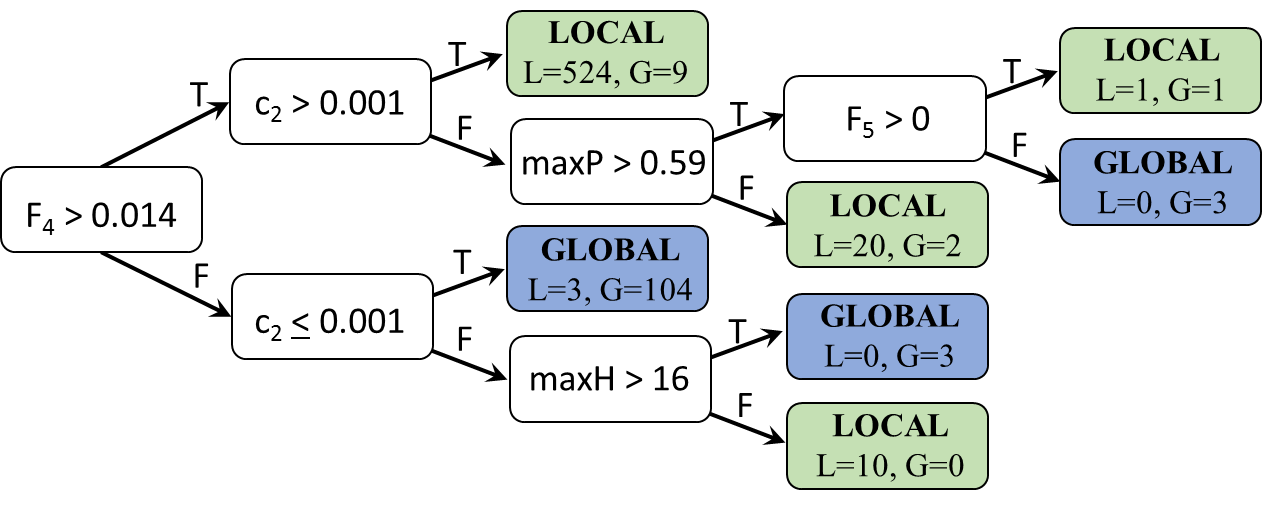
\includegraphics[width=5.9in]{Figures/DecisionTree.png}
 \caption[Global vs. Local Classifier]{Decision Tree Classifier for differentiating local vs. global influencers based on the features from account creation times of their followers. The number of local (L) and global (G) influencers predicted using each branch shown for each leaf node.}
\label{fig_decTree}
\end{figure}

\iffalse
The Decision Tree Classifier is shown below; after each branch the number of local (L) and global (G) influencers that end up as leaf nodes are shown:
{\fontfamily{pcr}\selectfont
\begin{tabbing}
in\=fluencer\_type\_decision\_tree($F_1$, $F_2$, $F_3$, $F_4$, $F_5$):\\
\> $F_4$ $(std(p24Dist))$ $> 0.014$: \\
\> |-- $F_3$ $(c_2)$ $> 0.001$: Local (L = 524, G = 9)\\
\> |-- $F_3$ $(c_2)$ $\leq 0.001$: \\
\> |-- |-- $F_1$ $(maxP)$ $> 0.590$: \\
\> |-- |-- |-- $F_5 > 0$: Local (L = 1, G = 1) \\
\> |-- |-- |-- $F_5 \leq 0$: Global (L = 0, G = 3) \\
\> |-- |-- $F_1$ $(maxP)$ $\leq 0.590$:  Local (L = 20, G = 2) \\
\> $F_4$ $(std(p24Dist))$ $\leq 0.014$: \\
\> |-- $F_3$ $(c_2)$ $> 0.001$:  \\
\> |-- |-- $F_2$ $(maxH)$ $> 16$: Global (L = 0, G = 3) \\
\> |-- |-- $F_2$ $(maxH)$ $\leq 16$: Local (L = 10, G = 0) \\
\> |-- $F_3$ $(c_2)$ $\leq 0.001$: Global (L = 3, G = 104) \\
end \\
\end{tabbing}
}
\fi

We used information gain to rank the features.  Top four features and their associated weights are:(i) $F_1$: 1, (ii) $F_4$: 0.983, (iii) $F_2$: 0.972, (iv) $F_3$: 0.956 (the weight for $F_5$: 0.058 so it is not as significant).

 As we have seen in the previous section, a sample of followers from a global influencer can lead to a time distribution that is unimodal, and for this reason, it is important to take a sample determined by Algorithm 1. Algorithm 1 searches for the optimal curve that is achieved if the peaks from time distributions are in sequence and contain all 24 hours; if the $\rho$ ($F_1$) is low and if a small number of hours ($F_2$) are covered this indicates a local influencer. 
%Based on the analysis of decision tree we note that 

If $F_4$ $(std(p24Dist))$ is low then the spatial  distribution is flat and belongs to a global influencer; which is consistent with observations made in the previous sections. The information gain identified that $F_3$ ($c_2$) less than 0.001 should be the cutoff for a global influencer (this exact value was also confirmed from analysis of stop words using message traffic in Section \ref{sec4}). Finally, if the time distribution is represented using only low order Fourier coefficients so that $F_5=0$ this means this is more of a flat line simple time distribution associated with a global influencer. %($FC_1$ had higher initial information gain, but after other features considered decision tree utilized $FC_4$).

This classifier is intuitive and over the whole dataset achieves 665/680 = 97.79\% accuracy. The followers of influencers that the classifier predicts as local %such as \emph{@BBCRussian} 
can be used for predicting UTC offset related to local expert finding in social networks. While the followers of global influencers %such as \emph{@BBC\_Travel} 
can be used for inferring daily follower gains and analyzing how their popularity has evolved.

\section{Conclusions} \label{sec7}

In this chapter, we have illustrated an approach for how creation times can be used in time series analysis. The creation times can stem from a group of messages or account creation times. It was illustrated that the distribution of creation times that stem from a single time zone %will form a time curve with a U-shaped valley. The U-shape 
will be approximately %paraboloidal
parabolic, with a minimum during the night time for that %corresponds to the time that the 
time zone. % experiences night. 
%By fitting a second degree polynomial the U-shape 
Regression with a quadratic function can be used to predict the UTC offset associated with the time zone. 
By examining message traffic, this information was utilized to identify trending keywords over %any
multiple geographic %area
areas of interest. 
In addition, by analyzing the set of followers of any influencer, we showed that this information can be utilized to determine how strongly localized is the range of influence
of an influencer. % is localized.
%to area of interest. 
This is useful for Location-Aware Influence Maximization (LAIM) and local expert finding in social networks. 

%By taking x followers at a time it was 
We also illustrated that a follower sample exists such that the peaks from multiple time curves occur in sequence. 
Analysis of variations of %the peaks %By plotting the peaks 
the wave pattern in the distribution of peaks
provides information %for studying
regarding the periodicity with which followers were gained. This is useful for understanding how an influencer's popularity has evolved over time, as well as for inferring link creation times.%, i.e.,   when a set of followers mentioned the influencer.

Finally, the proposed time-based features were utilized for creating a local vs. global type classifier. The classifier is important because the UTC offset prediction should be applied for local influencers whereas the analysis for how influencer's popularity evolved %over time 
works for global influencers.
